%% ---------------------------------------------------------------
%% $URL: https://repository.cs.ru.is/svn/thesis-template/trunk/ruthesis/latex/DEGREE-NAME-YEAR.tex $
%% $Id: DEGREE-NAME-YEAR.tex 360 2019-02-13 22:04:35Z foley $
%% This is a template LaTeX file for dissertations, theses, or reports at Reykjavík University
%% 
%% Comments and questions can be sent to the RU LaTeX group (latex AT list.ru.is) 
%% ---------------------------------------------------------------

%% METHOD:
%% 0) Read ruthesis/thesis-instructions.pdf
%%    If it is missing, goto https://repository.cs.ru.is/svn/thesis-template/trunk/ruthesis/thesis-instructions.pdf
%% 0.2) Subscribe to the announcements email list at
%%    https://list.ru.is/mailman/listinfo/latex-announcements
%% 1 LaTeX instructions.tex or goto http://afs.rnd.ru.is/project/thesis-template/trunk/ruthesis/latex/instructions.pdf
%% 2) Copy the template files (or unzip) to your working area
%% 3) Rename this file (if needed) with your information e.g. MSC-FOLEY-2007.tex
%% 4) Modify this file to fit your needs (please follow all comments below in the text)
%% 5) For making bibliographies, run "biber".  You can also change
%%    this back to "bibtex".  See below in "Bibliography options".

%%%%%%% CHOOSE ONE OF THESE %%%%%%%%%%%%%%%
%% projectreport: Project report (CS)
%% bachelors: Bachelor of Science thesis
%% masters: Master of Science thesis
%% doctorate: Doctor of Philosophy dissertation
%
%%%%%%% CHOOSE ONE OF THESE %%%%%%
%% 
%% draft: speed up processing by skipping graphics and adding useful
%%     information for editing.  Also sets spacing to double so that it is easier to
%%     write editing marks on paper copy.
%% proof:  proofreading version (final formatting with warnings)
%% final: generate document for submission, removing FIXMEs, and
%%     other markup.  Throw error if any fatal FIXMEs still in document.
%%
%%%%%%% CHOOSE ONE OF THESE IF APPLICABLE %%%%%%
%%
%% deptsse: School of Science and Engineering
%% deptscs: School of Computer Science
%%
%%%%%%%% CHOOSE ANY COMBINATION OF THESE %%%%%%%%%%%%
%%
%% forcegraphics: force graphics, etc. to be included, even in draft mode
%% debug:  writes more messages to the log file, adds debugging output 
%%     and sizing boxes
%% icelandic: thesis is in Icelandic
%% oldstyle:  use the PhD headers and footers from the old CS template
%% online: for online versions (skip blank pages)
\documentclass[online,masters,deptsse,forcegraphics,draft]{ruthesis}

%%%%%%%%%%%%%%%%%%%% TeXStudio Magic Comments %%%%%%%%%%%%%%%%%%%%%
%% These comments that start with "!TeX" modify the way TeXStudio works
%% For details see http://texstudio.sourceforge.neit/manual/current/usermanual_en.html   Section 4.10
%%
%% What encoding is the file in?
% !TeX encoding = UTF-8
%% What language should it be spellchecked?
% !TeX spellcheck = en_US
%% What program should I compile this document with?
% !TeX program = xelatex

%%%%%%%%%%%%%%%%%%%% Bibliography options %%%%%%%%%%%%%%%%%%%%%
%% We suggest switching from bibtex to biblatex/biber because it is better able
%% to deal with Icelandic characters and other bibliography issues
%% As long as you use biblatex instead of bibtex by itself, it will at least
%%  generate a document without errors.
%% !!!If you are using TeXStudio, don't forget to update the bibliography setting!!!
\usepackage[backend=biber,bibencoding=utf8,style=ieee]{biblatex}
%\DeclareLanguageMapping{american}{american-apa}  
% need to declare mapping for style=apa to alphabetize properly
% If you set backend=bibtex, it will use bibtex for processing (old way)
%    this can work with Icelandic characters, but you may get weird results.
%    bibtex does not know how to sort Þ and ð
% if you set backend=biber, you can use UTF8 characters such as Þ and
%     ð  but you will have to remember to switch from using bibtex to 
%     biber in your client
% If you use JabRef, make sure the file is encoded in UTF-8 which is
%    not the default.

%% This tells TeXStudio to use biber
% !TeX TXS-program:bibliography = txs:///biber
%% This also sets the bibliography program for TeXShop and TeXWorks
% !BIB program = biber

% Where is your reference library?

\addbibresource{zot-references.bib}

%%%%%%%%%%%%%%%%%%% CUSTOMIZATIONS %%%%%%%%%%%%%%%%%%%%%%%%%%%%%
%% It is not recommended that you customize this file nor
%% ruthesis.cls.  Just fill in the necessary fields.  You should put
%% your macros and packages into a separate file so that it is easier
%% to use updates to the template.  The custom.sty file was created
%% for this reason.  We load this much later so that it can overrite
%% any existing settings
\IfFileExists{custom.sty}{\usepackage{custom}}{}


%%%%%%%%%%%%%%% INFORMATION %%%%%%%%%%%%%%%%%%5
%% University information must be multilingual to deal with the
%%  required cover pages and abstract on thesis
%% NOTE: This may not be required for other reports!!!

%% Babel Icelandic macros are setup  on RedHat at
%% /usr/share/texlive/texmf-dist/tex/generic/babel/icelandic.sty
%% /usr/share/texlive/texmf-dist/tex/generic/babel-icelandic/icelandic.ldf


%% Multilingual macros
%\newML{macroname}{englishword}{icelandicword}
%  creates \macronameML
%    \MLmacroname[english] - returns the english word
%    \MLmacroname[icelandic] - returns the icelandic word
%    \MLmacroname  - uses the current language setting
% Some useful ones have already been defined, but can be redefined
%% Predefined: \MLIceland \MLReykjavikUniversity \MLUniversityIceland

%% What institute?  Default is RU.
%\setInstitution{\MLReykjavikUniversity}
% \newML{InstitutionAddress}{Menntavegur 1\\101 Reykjavík, Iceland}
% {Menntavegi 1\\101 Reykjavík, Ísland}
% \setInstitutionAddress{\MLInstitutionAddress}
% \newML{Tel}{Tel.}{Sími}
% \setInstitutionPhone{\MLTel{} +354 599 6200\\
% Fax +354 599 6201}
% \setInstitutionURL{www.ru.is}


%% ONLY SET DEPARTMENT IF YOU HAVE NOT USED THE deptsse or deptscs OPTION!
%% Department and degree program
%\newML{ND}{New Department}{Nytt deild}
%\setSchool{\MLND}

%% Set your program of study
\newML{program}{Mechatronics}{Hátækniverkfræði}
\program{\MLprogram}

%% Degree long name.  If not already defined, you can create a macro
%\newML{DEGREE}{English Degree Name}{Icelandic Degree Name}
%% Default is set based upon doctorate vs masters option
%% Predefined: \MLMSc \MLPhd
%\setDegreelong{\MLMSc}

%% Degree abb, change if default is not right
%% Default is set based upon doctorate vs masters option
%\degreeabbrv{Sc.D.} 

%\setFrontLogo{reyst-logo}
%% Use this if you need a different front logo on the first page
%% e.g. reyst-logo

%% Date in english and icelandic
%% NOTE: THIS IS THE DATE OF THE SUPERVISOR'S SIGNATURE!!!!!!
%% Predefined: \MLjan, \MLfeb, \MLmar, ... \MLdec
%\whensigned{day}{month}{year} %day is only used on some formats, but you must put something.
\whensigned{10}{June}{2021}

%% Title first in English then Icelandic
%% You need to put both a normal case and ALL CAPS version into the macros.
%%
\newML{Title}{Gathering sound data from cetacean creatures using a self-sufficient buoy}{Hljóðsöfnun á hvölum með notkun sjálfbærri bauju sem framleiðir sitt eigið rafmagn}
\newML{TITLE}{REYKAJVÍK UNIVERSITY PROJECT REPORT, THESIS, AND DISSERTATION TEMPLATE}{TITLL VERKEFNIS med ÞÖÆÉÍÓ}
%%
\setTitle{\MLTitle}{\MLTITLE}
%% ***** Special Titles ******
%% If the title must be formatted specifically for the cover page or internal pages
%% (typically via line-breaks using the \newline command) then the following commands must be used 
%%
%\setTitleCover{\MLTITLE}
%% These two for the internal cover pages, usually not needed
%\newML{TitleInternal}{Internal Title}{Icelandic Internal Title}
%\setTitleInternal{\MLTitleInternal}

%% Author name (should be the same in any language, if not use \newML)
%% If you are writing a Project report with multiple authors, separate them with \\:
%% To keep the names typeset together, you want to use non-breaking spaces: ~
%\author{Firstname1~Lastname1\\Firstname2~Lastname2}
\author{Sigurbergur~Magnússon}

%% If the name must be formatted specifically for the signature page
%% (typically via line-breaks) then the following command must be used 
%\setAuthorSignature{Student\\Name}
%% This macro adjusts the author name in the headers of the oldstyle formatting
%\setAuthorHeader{StudentLast}

%%% TODO:  Move the bachelor's form separately -- it confuses people. --foley
%%%%%%%%%%%%%%%%%%%%%%%%%% Project Report or Bachelor's Only!!! %%%%%%%%%%%%%%%%%%%%%%%%%%%%%%%%%%%%%%%%%%%
\setCourse{VT LOK 1012}

%%%%%%%%%%%%%%%%%%%%%%%%%% Bachelors Only!!! %%%%%%%%%%%%%%%%%%%%%%%%%%%%%%%%%%%%%%%%%%%
\setID{200594--2079}%kennitala
\setSemester{2016--1}
\setShortSignedDate{1.1.2016}

% \setOrganization{Marel ehf.\\Austurhrauni 9\\210 Garðabær}
% \setSubProgram{Tæknifræði}

%% If the thesis is confidential, uncomment this with the date it can be released
%\setClosedDistribution{10.1.2016}%

%% Put your keywords here in English, then Icelandic.  Separate them with commas.
\newML{keywords}{Keyword1, Keyword2, Keyword3}{Lykliorð1, Lykliorð2, Lykliorð3}
\setKeywords{\MLkeywords}

%%%%%%%%%%%%%%%%%%%%%%%%%%% Masters Only!! %%%%%%%%%%%%%%%%%%%%%%%%%%%%%%%%%%%%%%%%%%%%
%% How many credits (ECTS) on Master's degree
%% Usually 30 or 60
\ects{30}

%%%%%%%%%%%%%%%%%%%%%%%%%%% Doctorate Only!! %%%%%%%%%%%%%%%%%%%%%%%%%%%%%%%%%%%%%%%%%%
%% Some Computer Science Thesis have an ISSN number.
%% Most other documents do not.
%\bookidnumber{ISSN: 1670-8539} 
%% ID numbers are optional, but nice for sorting in libraries

%% International Standard Book Number (ISBN)
%% This is what most people should use if the thesis is being published.

%% International Standard Serial Number (ISSN)
%% This is usually only for a PhD dissertation as part of a series when published
%%   Computer Science: 1670-8539 

%% Additional degrees?  (optional, usually not needed)
%\adddegree{(list of degrees in appendix)}{(sjá lista yfir prófgraður í viðauka)}
%%%%%%%%%%%%%%%%%%%%%%%%%%%%%%%%%%%%%%%%%%%%%%%%%%%%%%%%%%%%%%%%%%%%%%%%%%%%%%%%%%%%%%%%


%% List the entire committee.  Each member has a name (degree should be omitted, unless it is not PhD),
%% Supervisor(s) must appear first
%% On a Bachelors, there is usually only one supervisor and one examiner.

%% Format for each entry:
%%  \personinfo{Name}{Role}{Job Title}{Company/institution}{Country}
%% Predefined macros: \MLSupervisor \MLSupervisors \MLExaminer \MLExaminers

%% Change these to singular/plural as needed.
%% Just uncomment and change the plurality of the macro.
%\setSupervisorHeading{\MLSupervisors}
%\setExaminerHeading{\MLExaminer}

%% Predefined macros:
%% \MLSeniorProfessor \MLProfessor \MLAssociateProfessor \MLAdjunctProfessor \MLEmeritusProfessor \Iceland
%% \MLReykjavikUniversity \MLUniversityIceland

%% Bachelors: primary advisor (Umsjónarkennari), ONLY ONE!
%% All others: As many as you want
\supervisors{
  \personinfo{Superior A. Teacher}{\MLSupervisor}{\MLProfessor}{\MLReykjavikUniversity}{\MLIceland}
%  \personinfo{Helpful A. Teacher}{Co-advisor}{\MLAssistantProfessor}{\MLUniversityIceland}{\MLIceland}
%  \personinfo{Ian M. Great}{Co-advisor}{\MLProfessor}{Hochschule Düsseldorf}{Germany}
}

%% Bachelors: secondary advisor (Leiðbeinandi), ONLY ONE
%% All others: As many as you want
\examiners{
  \personinfo{Tough E. Questions}{\MLExaminer}{Associate Professor}{Massachusetts Institute of Technology}{USA}

}

%% An abstract is required to be in both Icelandic and English for most degrees.
%% It is considered good form to limit the abstract to a single paragraph in each language,
%%   at 300 words.  Refer to your degree's instructions.
%% Note: Icelandic quotation marks cannot be typeset using "` and "'.  You should use \enquote{}
%% this is probably due to interactions with the MultiLingual macros.
%% TODO: turn this into more sensible macros to avoid confusion --foley
\newML{AbstractText}{\lipsum[1]}  
% ipsum generaes text text
{\lipsum[1]} % Icelandic abstract goes here
\setAbstract{\MLAbstractText}


%%%%%%%%%%%%%%INDEX SETUP %%%%%%%%%%%%%%%%%%%%%%%%%%%%%%%%%%%%%%%%%%%%%%%%%%%%
%% Indexes, and other auto-generated material
%% The Memoir package (which we use) automatically generates the index
%% See section 17.2 on page 302 of the guide
%% http://texdoc.net/texmf-dist/doc/latex/memoir/memman.pdf
%% This means you have to run "makeindex DEGREE-NAME-YEAR"
%% !!!Do not load any of the index packages, they cause problems with Memoir!!!
%% !!!You have been warned!!!
%% Note that memoir changes the [] options to only be for filenames, not other options!
\makeindex{}
\indexintoc{}

%% For abbreviations, you may want to try
%% Watch out though, each new index writes another external file and 
%% latex can only write a limited number of them
%%\usepackage[intoc]{nomencl} % intoc: In Table of Contents
%% remember to run:
%% makeindex filename.nlo  -s nomencl.ist -o filename.nls

\finalifforcegraphics{hyperref} %hyperlinks even in draft mode
\usepackage[hidelinks]{hyperref} 
%% !!!Must be the last package loaded except otherwise mentioned!!!!
%% \usepackage{hypcap}  %% puts link at top of figure, must be after hyperref

%%%%%%%%%%%%%%%%%%%%%%%%%%%%%%%%%%%%%%%%%%%%%%%%%%%%%%%%%%%%%%%%%%%%%%%%%%
%%%%%%%%%%%%%%%%%%%%%%% DOCUMENT START %%%%%%%%%%%%%%%%%%%%%%%%%%%%%%%%%%%
\begin{document}
%% Some elements have different names on the RU Masters rules
%% They will be annotated with RUM: "name"
\frontmatter{} % setup formatting at beginning

%\frontcover{}%%If you want to see what it looks like with the printed cover
%% TODO:  link to fill-in PDF file on RU website

\frontrequiredpages{}%% the various signaturepages and abstract
%%% WARNING:  if you get an error on the previous line, it is probably because
%%% you put a bad macro or something strange in a title, author, or abstract.

\ifdraft{\coverchapter{Important!!!  Read the Instructions!!!} If you
  have not already done so, \LaTeX{} the \path{instructions.tex} to
  learn how to setup your document and use some of the features.  You
  can see a (somewhat recent) rendered PDF of the instructions included in this folder at \path{instructions-publish.pdf}.
  There is also more information on working with \LaTeX{} at
  \url{http://samvinna.ru.is/project/htgaru/how-to-get-around-projects-publish.pdf}.
  This includes common problems and fixes.

  This page will disappear in anything other than draft mode.}{}



%% Dedication is optional, comment out if it is absent
%% RUM: Not mentioned
\begin{dedications}
  I dedicate this to my spouse/child/pet/power animal.
\end{dedications}

\enableindents{}% turn on/off paragraph indents
% RUM: "Acknowledgements (optional)"
\coverchapter{Acknowledgements} 
\begin{quotation}
So long, and thanks for all the fish.
\end{quotation}\sourceatright{Douglas Adams\cite{adams84fish}}
\vspace{\baselineskip}

\draftnote{Acknowledgements are optional; comment this chapter out if they are absent
  Note that it is important to acknowledge any funding that helped in the work}

This work was funded by \the\year~RANNIS grant ``Survey of man-eating Minke whales'' 1415550.
Additional equipment was generously donated by the Icelandic Tourism Board.

\coverchapter{Preface}
% RUM: "Preface (optional)"
This dissertation is original work by the author, Firstname~Lastname.
Portions of the introductory text are used with permission from
Student et al.\cite{student2015awesome} of which I am an author.

  
\draftnote{The preface is an optional element
  explaining a little who performed what work.  See
  \url{https://www.grad.ubc.ca/sites/default/files/materials/thesis_sample_prefaces.pdf}
  for suggestions.
  
  List of publications as part of the preface is
  optional unless elements of the work have already been published.
  It should be a comprehensive list of all publications in which
  material in the thesis has appeared, preferably with references to
  sections as appropriate.  This is also a good place to state
  contribution of student and contribution of others to the work
  represented in the thesis.}

%\coverchapter{Publications}
%% RUM: Not mentioned, this was found in the CS thesis template.  
%% Maybe more applicable to PhD dissertations?
%%% Probably a duplication from before Preface became standard.

\starttables{}% setup formatting
%% TOC, list of figures and list of tables are required
\tableofcontents{}\clearpage%%RUM: "Table of contents"
\listoffigures{}\clearpage%%RUM: "List of figures"
\listoftables{}\clearpage%%RUM: "List of tables"

%\coverchapter{List of drawings and enclosed material}
%RUM: "List of drawings and enclosed material, e.g. CD(as appropriate)"

\listoffixmes{}
% if using fixme package, lists what needs to be done


%% The list of abbreviations is an example of a special list
%% Other lists may be added, such as lists of algorithms, symbols, theorems, etc.
%% IN CS PhD, this is sometimes centered.

\coverchapter{List of Abbreviations}%%RUM: Not mentioned

\begin{tabular}{ll}
ADC &Analog to digital converter\\
DAC & Digital to anlaog converter\\
$dB$  & Decibels\\
MSc &Masters of Science\\
km &Kilometer\\
MMOs & Marine mammal observer\\
PAM & Passive acoustic monitoring\\
AAM & Active acoustic monitoring\\
DMON & Digital acoustic monitoring\\
LFDCS & Low‐frequency detection and classification system\\
DPS & Digital signal processor \\
I/O & Input/output\\
PWM & Pulse width modulation\\
IDE & Integrated development environment\\
KB & Kilobytes\\
GPIO & General Purpose Input/Output\\
RC & Resistor and capacitor\\
RMS & Root mean square\\
SPS & Samples per second\\
DCV & Direct current voltage\\
ADCK &ADC clock\\
OCRR & Open circuit receiving response\\
SIL & Sound intensity level\\
TVR & Transmitting voltage response\\
DMA & Direct Memory Access\\
PDB & Programmable delay block\\
ISR & Interrupt service routine

% PhD &Doctor of Philosophy\\
\end{tabular}

\coverchapter{List of Symbols}%%RUM: Not mentioned

\begin{tabular}{lll}
Symbol &Description &Value/Units\\
$E$ &Energy &\si{\joule}\\

$m$ &Mass &\si{gram}\\
$c$ &Speed of Light &\SI{2.99E8}{\meter\per\second\square}\\
$Hz$ & Frequency & Hz\\
$Ah$ & Ampere hour & 3600 coulombs\\
$F_c$ & Cutoff frequency & Hz\\

\end{tabular}

%% This command prepares for the actual text, e.g. by 
%% calling \mainmatter{}
\starttext{}

%% ---------------------------------------------------------------
%% From this point on, it is standard Latex, except the very end.
%% This is a "report"-based template, so the top-level heading 
%% is \chapter{}

%% WARNING: Make sure that all of these files (and any new ones)
%% are UTF-8 otherwise you will get weird encoding errors.
\part{The First Part} % Parts optional but useful in longer documents
Introduction to the first part.
%% The default division is IMRAD, you may want to divide differently
%% See the introduction for guidance.




\chapter{Introduction\label{cha:introduction}}
%% \ifdraft only shows the text in the first argument if you are in draft mode.
%% These directions will disappear in other modes.

% \ifdraft{State the objectives of the exercise. Ask yourself:
%   \underline{Why} did I design/create the item? What did I aim to
%   achieve? What is the problem I am trying to solve?  How is my
%   solution interesting or novel?}{}

% The object of the project is to be able to monitor cetacean traffic around Iceland.
% This could help tourism companies relating to whale watching. 
% Could also be extended to whale researchers.


Humans have caused increased pressure on animals whether that be land or sea creatures.
Keeping track of the creatures is vital to ensure their health and survival for the future.
This can be done by population assessments, which can show if the specific species is in an upsurge or declining in terms of numbers.
For fish and cetaceans, there are several ways to achieve this for example the animal can be tracked via Global Positioning System (GPS) tracker or the animal is visually sighted by the use of a boat or aircraft.
These methods are however time consuming and require a lot of man power.
To plant a tracker on the animal it must first be found and captured in order to attach the tracker and the later method requires researchers to actively search the animal, which is heavily reliant on favourable sea conditions etc.
There is however methods available that rely on acoustic surveys in order to monitor cetaceans which enables researchers to not only explore the surface of the ocean but also beneath the waves.
These surveys can be done in several ways.
One method involves dragging an array of hydrophones and record the vocalization data.
The second is to mount hydrophones into the bow of the ship and record the vocalization data.
These method however can not be used when recording low frequency sounds, due to noise created by the ship and water flow as well as still requiring researchers on board ships actively looking for animals.
The third method, and the one this thesis will focus on is a passive buoy sound gathering.
Where a hydrophone and a recording device are attached to a buoy that moored in place and sets on recording passively that location without the need of external help and maintenance.

The buoy must be self sufficient and able to stay out at sea for long periods at a time to serve its function.
This means that all the electronics on board will need to be powered by the buoy.
It also has to be able to record cetacean vocalization and transmit the data onshore.
So that marine researchers can study the data or even whale watching companies in the tourism industry can play cetacean vocalizations in the fjords.
This means the passive sound gathering buoy can be separated into three different projects, power production, sound gathering and data transmission onshore.
This thesis will focus on developing a device for the cetacean vocalization recording.

This function will be implemented using a Teensy 3.5 microcontroller.
A hydrophone will be used in order to sense the sound waves generated by the cetacean vocalization which have an extremely wide frequency range of a few Hz all the way to echolocation signals which are hundreds of thousands of Hz, this project will have therefore gather signals in the range of 10Hz to 100kHz, at at least 16bits resolution for high quality audio.
The electrical circuit will consist of a preamplifier, filter, analog to digital converter and SD card for data logging.
The circuit will refine the signal to be readable for the microcontroller. 


\section{Project Goals}

The objective of the project is to create a relatively small, low cost and low maintenance device capable of recording cetacean vocalization and transmitting the data onshore.
The design criteria for the project is as follows.
The total power consumption to the system should be less than 10 watts. 
The device should be relatively small and lightweight,so it is deployable by one person.
The device should last 6 months at a time.
Maximize the frequency at which the device is able to record.
%Be able to gather data of signal ranging from 10Hz to 100kHz. \fxfatal{Skoða aðeins betur}
\clearpage

\section{Background}

Considerable cetacean preservation efforts have been carried out for the past decades.
In 1946 the International whale commission, which is a global body with the goal of conservation of whales and currently has 88 member governments from all over the world.
Which is a global organization with the goal of conserving and managing whales and it currently has 88 countries signed to the committee \cite{noauthor_iwc_nodate}.

Many methods have been used to monitor the population of cetaceans.
These methods range from very active hands-on surveys where Marine Mammal Observers (MMOs) capture, examine, mark and then let the animal go to be recaptured in the future.
To a more passive acoustical surveys where hydrophones are utilized to listen in on cetaceans.

%https://www.sciencedirect.com/science/article/pii/S0003347216301452#:~:text=We%20describe%20several%20methods%20developed,high%2Dresolution%20acoustic%20recording%20tags.

\subsection{Visual surveys}% and photogrammetry 

Visual surveys are generally carried out by the use of  boats, helicopters or airplanes.
Trained marine researchers use high power binoculars to search for cetaceans breaching the surface of the ocean.
Once the cetacean is sighted it is categorised accordingly with regards to the study.
Immense data can be extrapolated from such research such as the location of the sighting, the species sighted, group size to name a few\cite{campbell_inter-annual_2015}.
How ever there are several factors that might limit or stop a visual survey such as sea conditions, visibility, the behaviour of the animal.
As well as the countless other animals that could lie just beneath the surface out of MMOs sight.

\subsection{Hands-on surveys}

This method utilizes animals that are caught and released, animals that are being cared for and animals that have become incapacitated by beaching. 
Animals that are caught are identified, which can be done by taking photographs of markings or identifying features, that in the future could be used to identify it if the animal is ever recaptured.
This is known as photo-identification\cite{booth_methods_2020}.
This approach has been utilized in order to gain a further understanding on population and health of cetaceans.

Individual tracking surveys are similar in the fact that the animal is captured and released in the same manner.
However instead of taking photographs of it before releasing it, the animal would have a GPS tracker attached to it. 
Which has been utilized for research into acquiring data regarding behaviour and responses of disturbance sources as well as data on the animals travel and habitat patterns. 
Depending on what the researcher wants to get data on will dictate on whether or not the GPS tracker is added on to the animal\cite{booth_methods_2020}.



\subsection{Acoustic surveys}

Methods previously mentioned rely heavily on favorable conditions regarding sea conditions, weather and visibility since the MMOs need to be able to spot the cetaceans.
There are different methods to conduct the surveys, which can fall in one of two categories either active or passive.
Active acoustic monitoring (AAM) includes systems such as fish sonars and echo sounders. 
Cetaceans are detected with target reflection instead of vocalization \cite{pyc_evaluation_2015}.
Passive acoustic monitoring (PAM) relies on the use of hydrophones, where cetacean vocalizations are recorded and studied.\\
\indent There are several methods to choose from when conducting a PAM.
The first method involves towing an array of hydrophones behind a vessel at sea such as ship and recently autonomous platforms have been utilized instead\cite{baumgartner_diel_2008} .
This however still requires favourable sea- and weather conditions, as well as when a ship is used there still needs to be active MMOs on board.
Another is to mount hydrophones in the bow of the ship.
This method is however limited frequency range due to the noise created by the ship bow and water flow\cite{rankin_acoustic_2008}.
The third is to have a fixed device, that has hydrophones and is able to either store vocalization data on the device itself or transmit the data directly on shore to researchers.
These devices are generally capable of long term unmanned monitoring and can be a quite cost effective alternative.
All three methods can eliminate most if not all of the previously described problems that can occur with visual surveys.



\subsection{Devices currently available}
\subsubsection{$\mu$RUDAr-mk2}

Devices such as the $\mu$RUDAR-mk2 as seen in \textit{Figure~\ref{fig:uRUDAR}}, is a product from Cetacean research technology that offers a remote fixed monitoring system.
It has the ability to remote autonomous recording.
WiFi recording control and data transmission capability.
The device is able to record up to 24-bit/96kHz and 45kHz bandwidth and up to 16.5 days of continuous recording time\cite{computing_microrudar_nodate}.
This device however relies on battery power and cant generate electricity and therefore has limitations on deployment time.

\begin{figure}[h]
    \centering
    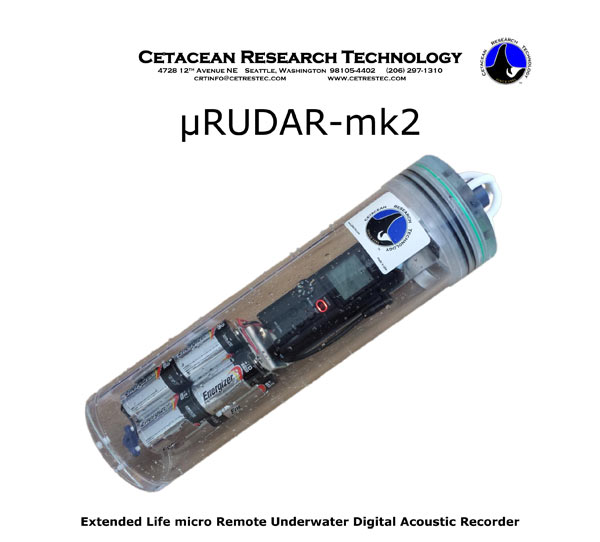
\includegraphics[width=0.70\textwidth]{graphics/uRUDAR-mk2.jpg}
    \caption{uRUDAR-mk2 fixed monitoring device\cite{computing_microrudar_nodate}}
    \label{fig:uRUDAR}
\end{figure}

\subsubsection{RUDAR (Remoter Underwater Digital Acoustic Recorder)}
Another recording device from Cetacean research technology is the RUDAR (Remoter Underwater Digital Acoustic Recorder), seen in \textit{Figure~\ref{fig:Rudar}}. 
It is a autonomous recording device that is small enough to be hand deployed from a small boat.
The recording system uses the ST400 mobile data recorder and sound level monitor. 
The system has a working depth of 1.5-3.5km it is able to record from 4 hydrophones at 24-bit resolution.
The data is written to an internal hard drives and is able to record 2 independent schemes and sample rates at the same time \cite{cetacean_research_technology_rudar_2021}.

\begin{figure}[h]
    \centering
    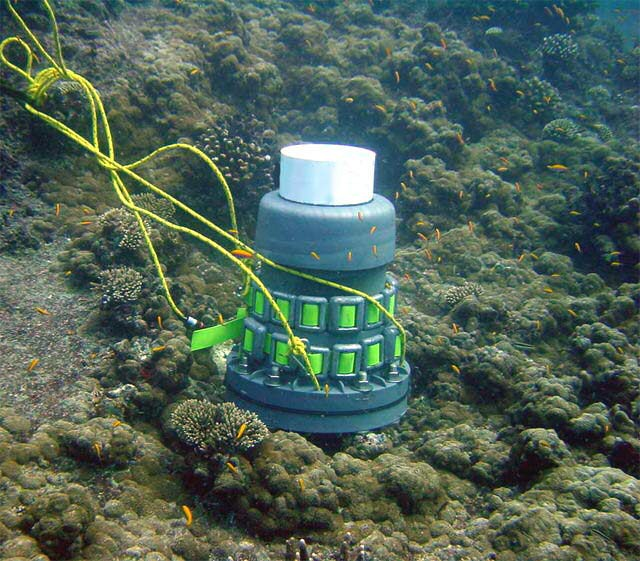
\includegraphics[width=0.70\textwidth]{graphics/Rudar.jpg}
    \caption{RUDAR recording device \cite{cetacean_research_technology_rudar_2021}}
    \label{fig:Rudar}
\end{figure}

%\fxfatal{TALA KANSKI UM F-pod hér \cite{noauthor_f-pod_nodate}}

\subsubsection{Persistent near real‐time passive acoustic monitoring for baleen whales from a moored buoy.}
A system has been developed for the United States Coast Guard that is capable of long term remote deployment. 
The system consist of a moored buoy that can provide data collection and transmission.
It has passive acoustic instruments such as digital acoustic monitoring(DMON) and a low-frequency detection and classification(LFDCS) firmware.
The system has three hydrophones and a a programmable Texas Instruments TMS320C55 digital signal processor (DPS) as well as GPS.
The firmware is used to build a spectogram of the recorded sounds when the mooring is recovered.
An example of which can be seen \textit{Figure \ref{fig:SpectoExamp}}.
It then classifies the sound calls by comparing attributes of the pitch track to known call types. 
The mooring hardware of the surface buoy is used for power delivery as well as data transmission. 
The system has an internal battery capacity of 450 Ah. 
%The audio is recorded with a sample frequency of 2kHz. 
It is designed to operate for a period of 1 year at a time has a maximum data transfer rate of 8Kb per hour through Iridium global communication system \cite{baumgartner_persistent_2019}.

\begin{figure}[h]
    \centering
    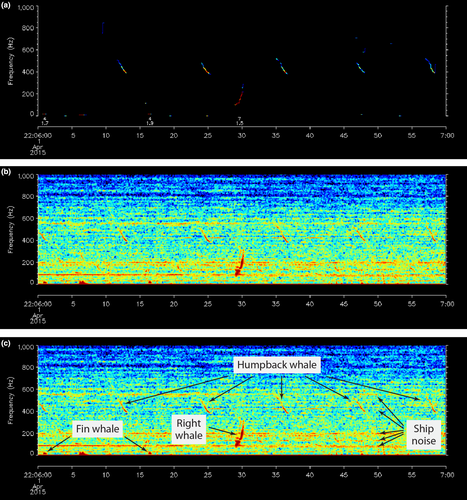
\includegraphics[width=0.60\textwidth]{graphics/spectogram.png}
    \caption{Spectogram that can be produced once the mooring is recovered.
    (a) In near-real time detection information (b) spectogram for a the given time period seen in (a) at 2000Hz sampling rate (c) addition of annottations of sound source to spectogram seen in (b)\cite{baumgartner_persistent_2019}}
    \label{fig:SpectoExamp}
\end{figure}

The setup of the of the system can be seen in \textit{Figure~\ref{fig:DMON/LFDCS}} from the moored surface buoy at the top, to the monitoring device at the bottom of the ocean.

\begin{figure}[h]
    \centering
    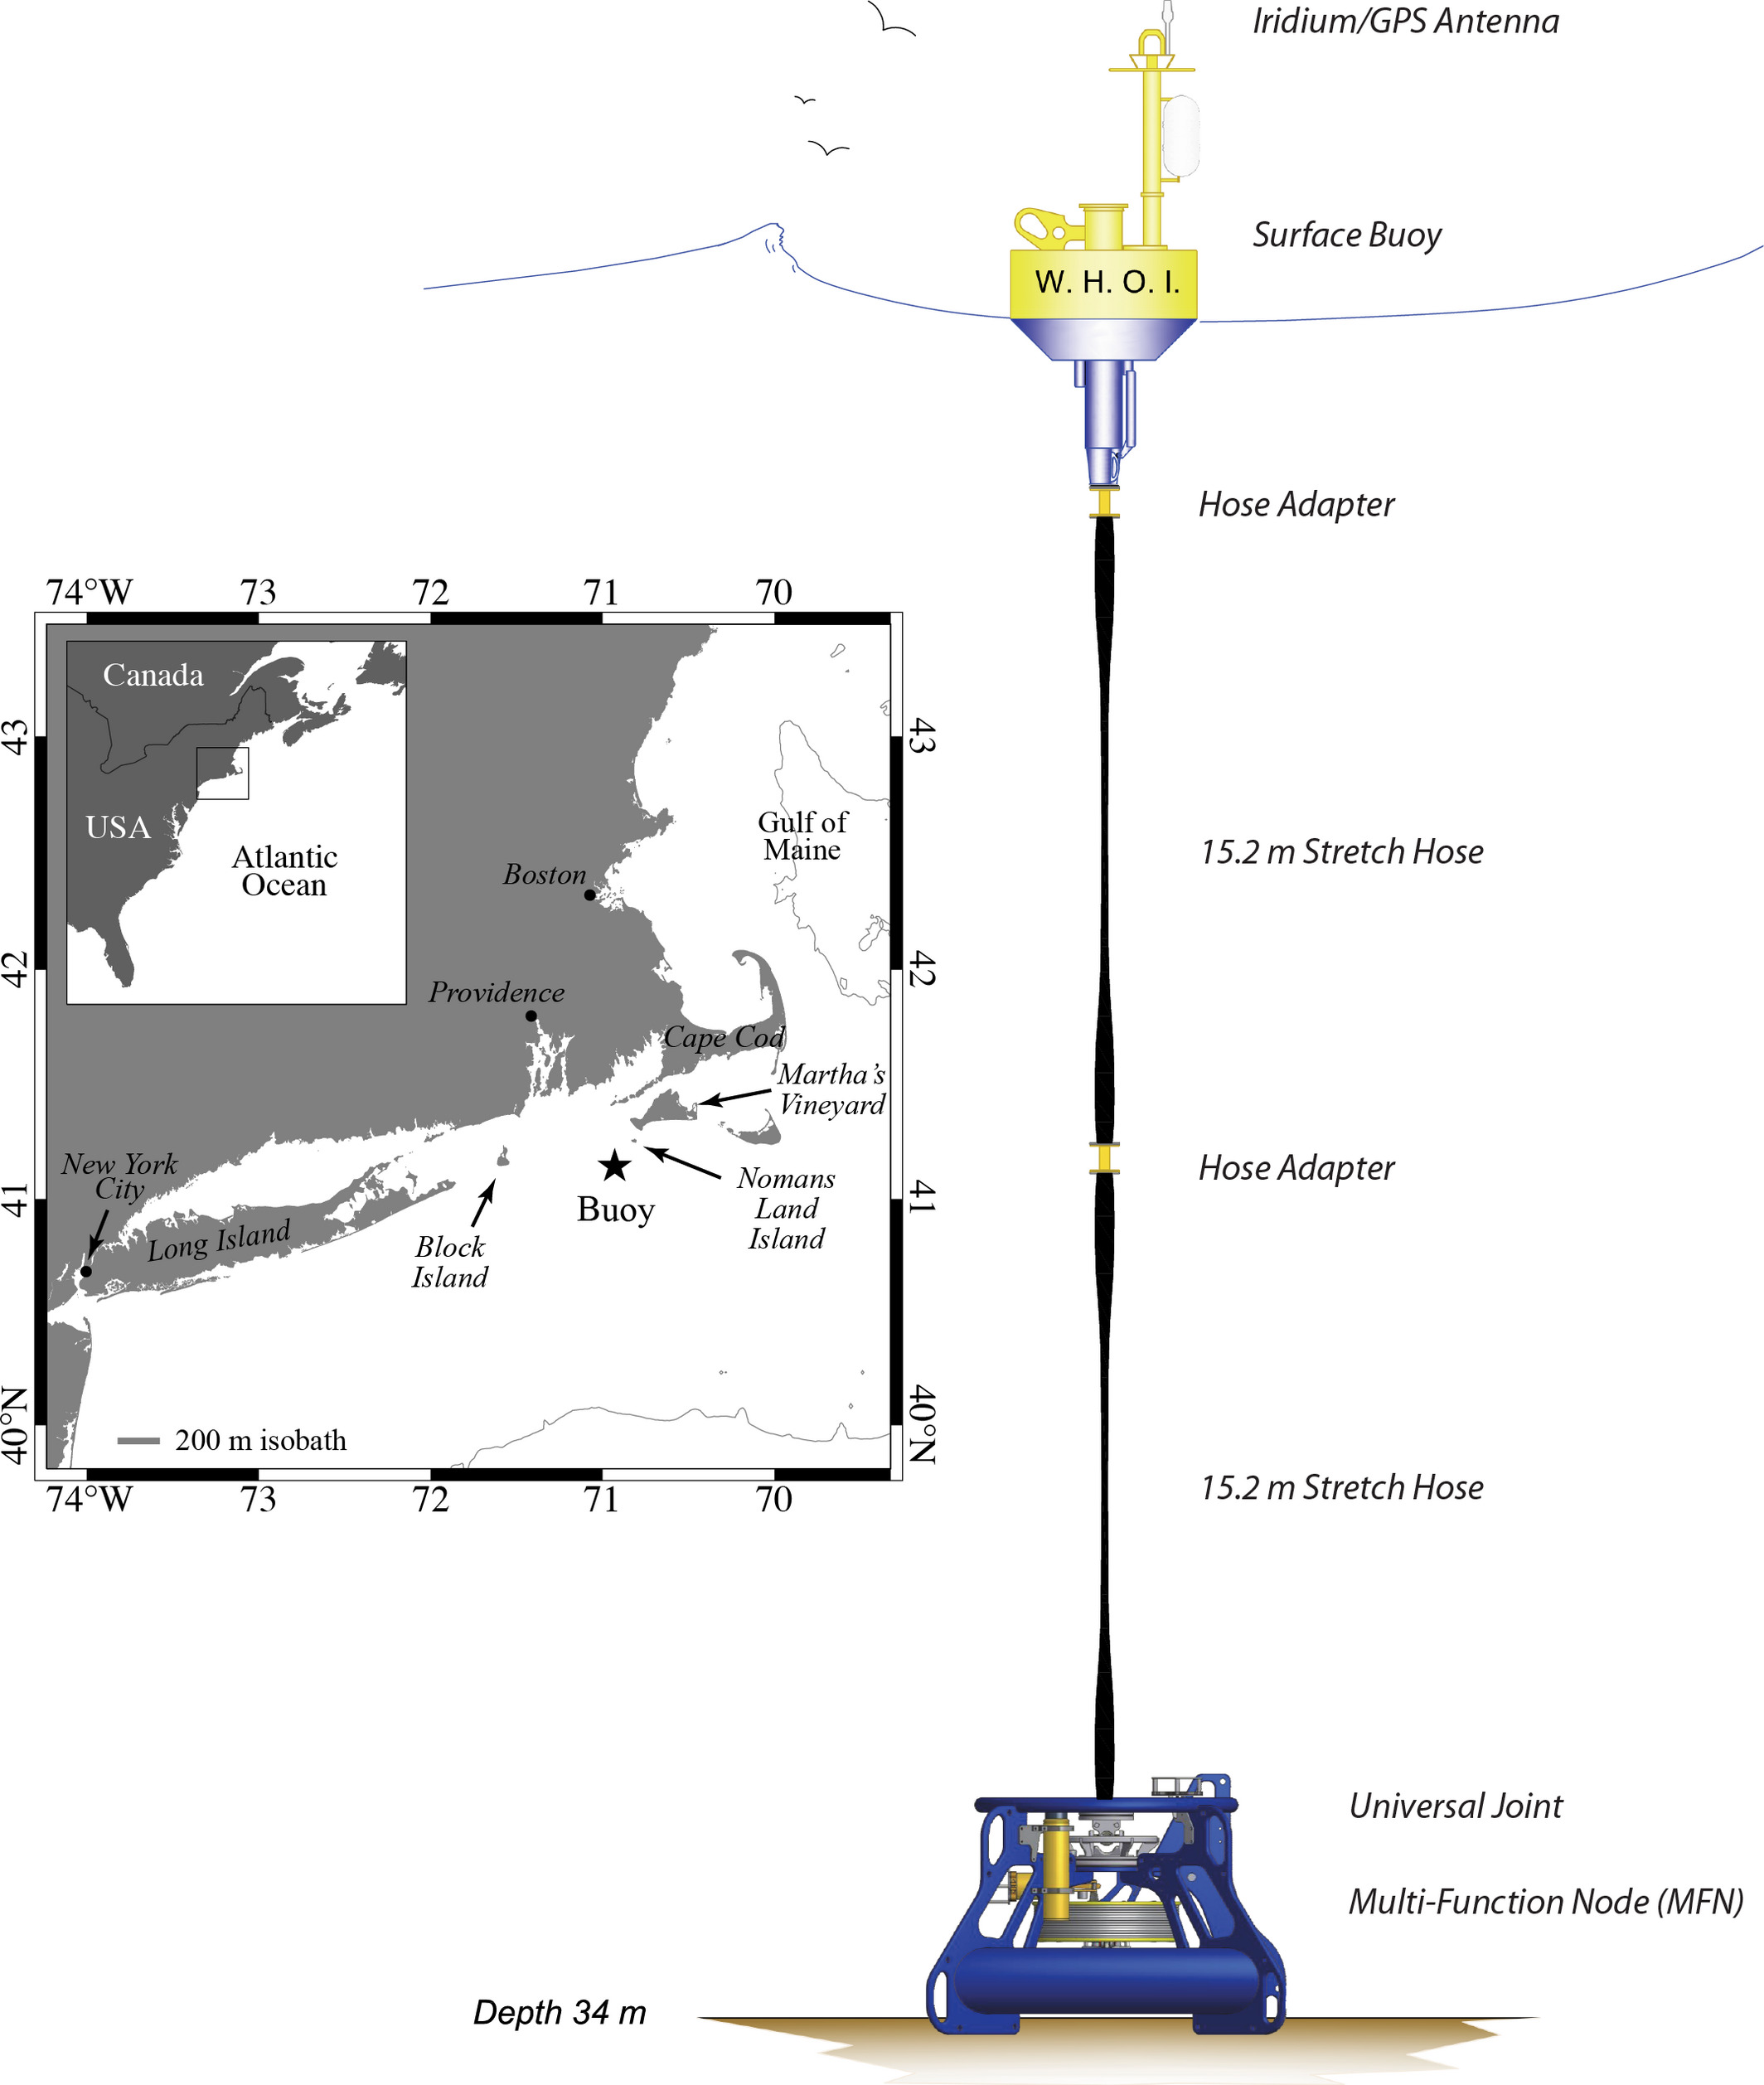
\includegraphics[width=0.70\textwidth]{graphics/DMONbuoy.jpg}
    \caption{A moored buoy using DMON/LFDCS systems, designed for 1 year deployments\cite{baumgartner_persistent_2019}}
    \label{fig:DMON/LFDCS}
\end{figure}

\clearpage


\subsection{Cetacean vocalization}

Many different species of cetaceans can be found near Iceland.
There are at least 12 species that roam Icelandic oceanic waters.
Among which are most frequently spotted are harbour porpoise, white beaked dolphins, minke whales and humpback whales \cite{user_whales_nodate}.
Sound is used by cetaceans for various purposes the low frequency sounds are used for communication and high frequency prey hunting, predator avoidance as well as echolocation for navigation \cite{nowacek_studying_2016}.
Each species can vocalize different sounds.
The sounds can be described as moans, calls, clicks, shrieks and more\cite{greenhow_hearing_nodate}.
%Cetaceans use these sounds to low frequency sound for communicating to one another all the way to creating high frequencies echolocation sounds for hunting their prey\cite{greenhow_hearing_nodate}.
\textit{Table \ref{Tab:WhaleHz}} shows the type of sound, frequency range of the sound, the dominant frequency of the sound and the source level of each sound for its respective species.

Cetaceans produce vocalization and echolocation sounds with a wide bandwidth, or 2 - 150kHz as seen in \textit{Table \ref{Tab:WhaleHz}}.
In comparison humans have vocalization range of up to 5kHz and a hearing range from 16Hz - 20kHz \cite{monson_perceptual_2014}.
The vocalization can be so powerful that the low frequency sounds might be able to travel thousands of kilometers\cite{nowacek_studying_2016}.
The energy of sounds from for example killer whales, in calm seas can travel up to 25.9km.\cite{miller_diversity_2006}.

\newpage

\subsection{Audio}

\subsubsection{Sound waves}

Sound is a mechanical vibration, which results in an oscillating wave.
The wave causes a change in pressure of molecules 
The wave can travel through gasses, liquids and solids.
It occurs when objects vibrate, such as a diaphragm of a speaker or a vocal cord of a human.
It is a wave that has a frequency and amplitude, which determines the type of sound and the intensity of the sound.
Sound waves behave very differently in liquid and in air.
In liquid such as sea water there are several things that affect sound propagation.
Such as the sound can bounce off particles or other sea creature and even the bottom and the surface of the sea which causes reflection to the sound waves and cause energy loss.
Finally and the largest factors are depth, salinity and temperature of the water .
These factors can distort the sound and create transmission losses\cite{noauthor_sonar_nodate}.
Speed of sound is quite different whether it is traveling in air or in the ocean.
Speed of sound for example in 20°C air is roughly 343m/s, while  in the ocean it a lot faster and can vary around 1500m/s depending on the temperature, pressure and salinity of the ocean. 

\begin{figure}[h]
    \centering
    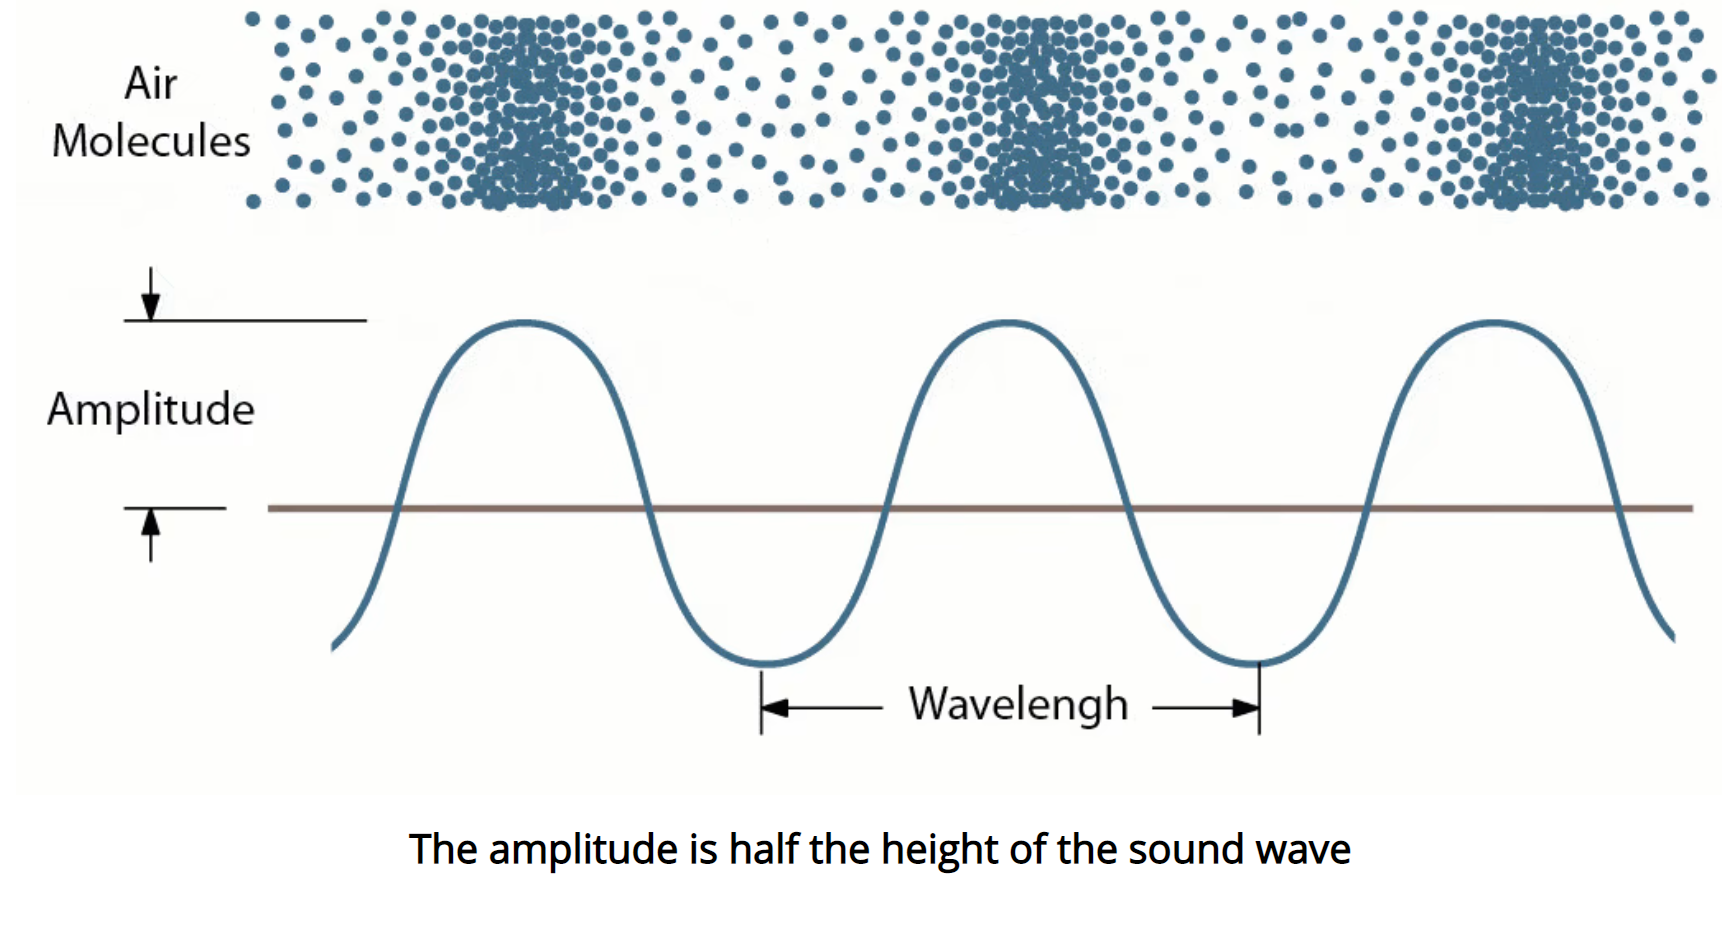
\includegraphics[width=0.70\textwidth]{graphics/soundwaves.png}
    \caption{How molecules react to sound waves \cite{noauthor_what_nodate}}
    \label{fig:SoundWaves}
\end{figure}

\subsubsection{Digital audio recording}\label{sec:DigitalAudiRec}

%https://documentation.meraki.com/MR/WiFi_Basics_and_Best_Practices/Signal-to-Noise_Ratio_(SNR)_and_Wireless_Signal_Strength#:~:text=The%20SNR%20is%20the%20difference,signal%20and%20the%20noise%20floor.&text=For%20example%2C%20if%20a%20client,dB%20for%20this%20wireless%20connection. - SNR

Audio recording is the recreation of sound waves, which can either be analog- or digital recorded.
Digital recording is the process of converting analog sounds, which means converting the analog signals from a microphone to a digital format. 
Which is done by representing the audio signal with binary numbers, which represents the amplitude or intensity of the sound and then sampling or recording that sound at a given time interval.
The greater the resolution the less noise is being recorded.
Resolution is determined by the number of bits used in order to record a signal and deter the precision of the measurements, it is the smallest incremental voltage change that can be recognized.
For example if a signal had a voltage range from 0 - 3.3V and it was being recorded at 16bits the voltage resolution would be $\frac{3.3V}{2^{16}} = 50\mu V/bit$.
Which would mean that the recording could in theory have $50\mu V$ increments in representing the signal.  
While a 8bit resolution only yields $\frac{13mV}{bit}$, meaning the higher the resolution, the more precise the measurement values are.
However with more bits comes more data rate and higher storage requirements.

\begin{equation}
    Data Rate = \frac{Bits}{8} * Sampling Rate * Number of channels 
    \label{eq:dataRate}
\end{equation}

Data rate can be calculated using \textit{Equation~\ref{eq:dataRate}}.
Where bits is the resolution, sampling rate is the sampling frequency in Hz and the number of channels is how many signals are being recorded.
The data rate can then be used to determine the amount of storage needed.
Nyquist-Shannon theorem is is in digital recording to determine the minimum sampling rate needed to reconstruct the analog signal.
The theorem proves that if the sampling frequency is twice the frequency of the highest frequency of the input analog signal, the signal can be recreated exactly.% \cite{bartlett_practical_2016}.
So in theory since humans have a hearing range of up to around 20kHz, in order to reconstruct all signals that are audible to humans, the sampling rate needs to be at least 40kHz.
For example on CDs the quality of the recording is 44.1kHz/16bits, in DVDs it is 96kHz/24bits and for high end audio recording it can go to 192kHz/24bits.
The oversampling can improve the recording for more accurate recording.
But oversampling is a term used for when the sampling frequency is of a higher rate than the Nyquist-Shannon theorem states  \cite{bartlett_practical_2016}.
If for example a sampling frequency of 200kHz was used when the signal being recorded was 20kHz it would be considered 5x oversampling.
The frequency that controls the ADC conversions also has to be precise.
If the timing of the samples is unstable it is called jitter, which is the standard deviation from the mean of the clock used to control ADC conversions.
The difference in decibel between the signal and the noise floor is called signal to noise ratio (SNR), meaning the difference between the input signal and the no signal is the SNR.
For cleaner sounds, meaning less noise is audible and more of the actual signal of interest, the higher the SNR.
Generally it is considered fair if the SNR is 60dB, good if SNR is 70dB and great if its 80dB or more \cite{bartlett_practical_2016}.


%\section{Device hardware}

%\textbf{FARA 'I GEGNUM VERKEFNI SEM AÐRIR HAFA GERT RUNNA ÞAU OG TALA UM NIÐURSTÖÐUR OG DÆMA HVÐ VIRKAR HVAÐ EKKI OG AFHVERJU ÞETTA GETUR VERIÐ EH APPENDIX DÆMI}

\subsection{Hydrophone}

Hydrophones are devices specially designed for underwater sound recording.
One of the earliest known examples of a hydrophone was made by stretching a membrane tightly over the end of a tube, one end of the tube is placed underwater while the other end is placed to the observers ear \cite{wood_a_b_textbook_1946}. 
Modern hydrophone are mainly based on piezoelectric transducers.
These hydrophones have been used since the early stages of world war 1.
Paul Langevin developed the first piezoelectric hydrophone, which was intended to be used for the detection of submarines.
A vacuum tube amplifier in combination with a piezoelectric material to be used as a transducer signal\cite{van_der_kloot_great_2014}.

When choosing a hydrophone it is important to look at a few specifications in the data sheet of the hydrophone. 
Such as the open circuit receiving response (OCRR), which is what the transducer outputs in terms of dB re 1V/$\mu$Pa.
As well as the frequency range that the hydrophone can receive and how much amplification it needs for different applications.
Also some things to consider is things like
%Which is function of frequency and expressed in terms of dB re 1V/$\mu$Pa.
sound intensity level (SIL) is the intensity of the sound at the transducer and is expressed in terms of dB re $\mu$Pa.
As well as transmitting voltage response (TVR) is the output voltage of the SIL at 1m range from the transducer and is expressed in terms of dB re $\mu$Pa/1V @ 1m \cite{ethem_mutlu_sozer_underwater_nodate}. 
Usable frequency of the hydrophone, directional patterns of the hydrophone and if the it applies the nominal capacitance of the hydrophone are also important factors. 
If for example the CRT C57 hydrophone was chosen, specifications can be seen in \textit{Table \ref{Tab:CRT57Hydrip}}.

\newpage

\begin{table}[h]\caption{Specifications of CRT C57 hydrophone range \cite{computing_c57_nodate}}.\label{Tab:CRT57Hydrip}
\centering
\begin{tabular}{|r|c|c|}
\hline
\multicolumn{1}{|c|}{\textbf{}} & C57 / C57X & C57RS/C57XRS \\\hline
{\begin{tabular}[c]{@{}r@{}}Linear Frequency Range \\ (±3dB) {[}kHz{]}\end{tabular}}      & 0.015 to 45         & \begin{tabular}[c]{@{}c@{}}0.015 to 50\&\\ 124 to 250+\end{tabular} \\ \hline
{\begin{tabular}[c]{@{}r@{}}Usable Frequency Range \\ (+3/-12dB) {[}kHz{]}\end{tabular}}  & 0.008 to 100        & { 0.008 to 77 \& 96 to 250+}                    \\ \hline
{\begin{tabular}[c]{@{}r@{}}Transducer Sensitivity* \\ {[}dB, re 1V/µPa{]}\end{tabular}}  & -187                & { -200}                                         \\ \hline
{Preamplifier Gain {[}dB{]}}                   & 20 / 33             & { 20 / 33}                                      \\ \hline
{\begin{tabular}[c]{@{}r@{}}Effective Sensitivity*\\  {[}dB, re 1V/µPa{]}\end{tabular}}   & -167 / -154         & { -180 / -167}  \\  \hline
\multicolumn{1}{|l|}{\begin{tabular}[c]{@{}l@{}}Price from dealer \\ {[}€{]}\end{tabular}} & \multicolumn{1}{|l|}{1290/1290} & \multicolumn{1}{|l|}{1290/1290} \\ \hline
\end{tabular}
\end{table}

If the CRT C57RS has an OCRR of -200 db re 1V/$\mu$Pa over a frequency range of 0.008 to 77kHz. 
Lets say a Blue whale is producing a moan which from \textit{Table \ref{Tab:WhaleHz}} indicates that the SIL would be 188dB re $\mu$Pa.
Then $VdB = SIL + OCRR = 188 + (-200) = -12dB$.
Because VdB is relative to 1V, the voltage output can be described as $V = 10^{VdB/10}$
which means the voltage output of the hydrophone would then be $V = 10^{-12dB/10} = 63mV$ and with the preamplifier of 20dB the $V = 10^{8dB/10} = 6.3V$.

% Converting the oscillating mechanical pressure difference (sound waves) to electrical energy \cite{li_piezoelectric_2012}.
% https://www.researchgate.net/publication/255001750_Piezoelectric_Materials_Used_in_Underwater_Acoustic_Transducers
% https://archive.org/details/in.ernet.dli.2015.15768/page/n471/mode/2up
% https://en.wikipedia.org/wiki/Hydrophone#cite_note-3
%https://se.mathworks.com/help/phased/ref/phased.isotropichydrophone-system-object.html

\subsection{Signal conditioning}

Conditioning the output signal produced by the hydrophone is important in order to only monitor only desired frequencies but also to have the voltage output in the correct range designed for the device.
Unwanted frequencies need to be filtered out in order to get a cleaner signal in the range that is desired.
In lower frequency application, from 0 - 100kHz a simple resistor and capacitor (RC) filters can generally be used \cite{noauthor_low_2013}.
The cut off frequency ($F_c$) point is defined when the output signal is 70.7\% of the input, which is when the the voltage gain is at -3dB = $20log(\frac{V_{out}}{V_{in}})$.
High pass filters works by filtering out frequencies that are lower than the set $F_c$ and allows frequencies higher to pass through.
%The $F_C$ point is defined when the voltage output signal is 70.7\% of the input, which is when the output signal is -3dB that of the input.% = $20log(\frac{V_{out}}{V_{in}})$.
Low pass filters out higher frequencies than the set $F_c$ and allows frequencies that are lower to pass through. 
For first order filter this occurs at a rate of -20dB/Decade after the set $F_c$, the slope of which can be increased by increasing the order of the filter.
Examples of the RC filters can be seen in \textit{Figure \ref{fig:PassiveHighLow}}.


\begin{equation}
    F_c = \frac{1}{2\pi RC}
    \label{eq:FC}
\end{equation}

To find the cutoff frequency of a first order filter circuit \textit{Equation \ref{eq:FC}} can be used.
Where $R$ is the resistor value in $\Omega$ and $C$ is the capacitor value in farads $F$.
Since the filter contains a capacitor the output signal will lag behind the input signal and shifts phase compared to the input. 
The capacitor takes time to charge and causes a lag between the input and the output voltage \cite{noauthor_low_2013}. 

\begin{equation}
    \theta = \arctan(2 \pi fRC)
    \label{eq:phasshift}
\end{equation}

The phase shift angle can be found using \textit{Equation~\ref{eq:phasshift}}.
Where $\theta$ is the phase shift angle, f is the frequency of the input signal, R is the resistor value on $\Omega$ and C is the capacitor value in Farads $F$.

The time constant of the capacitor which is caused by the charging and discharging effects of the resistor and capacitor gives the circuit a response in the time domain. 
Which is the elapsed time for the circuit to respond to changes in the the input signal of the circuit.


\begin{equation}
    \tau = RC = \frac{1}{2\pi F_c}
    \label{eq:Tau}
\end{equation}

The time constant of the RC filters can be found using \textit{Equation~\ref{eq:Tau}}. 
Where $\tau$ is the time constant, R is the resistor value on $\Omega$ and C is the capacitor value in Farads $F$ and $F_c$ is the cutoff frequency. 

\begin{figure}[h]
    \centering
    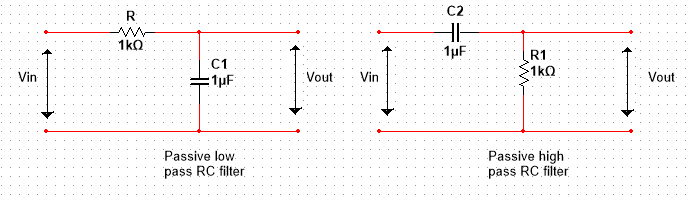
\includegraphics[width=0.70\textwidth]{graphics/passivehighlow.png}
    \caption{Passive low and high pass filters RC filter setups.}
    \label{fig:PassiveHighLow}
\end{figure}

Operational amplifiers or op amps are device that amplify voltage signals.
These devices are heavily used in all kinds of signal conditioning and filtering.
The gain of op amps is a ratio between the input voltage and the output voltage. 

\begin{equation}
    A_v = \frac{V{out}}{V{in}} = 1 + \frac{R_f}{R_{in}}
    \label{eq:DCGain}
\end{equation}

The gain from a non inverting op amp can be found by \textit{Equation \ref{eq:DCGain}}, $A_v$ is the gain and $R_f$ and $R_{in}$ are the resistor values of the resistor configuration seen on the right hand side in \textit{Figure \ref{fig:invNonInvOPamp}}.


\begin{equation}
    A_v = -\frac{V{out}}{V{in}} = -\frac{R_f}{R_{in}}
    \label{eq:invertDCGain}
\end{equation}

The gain from an inverting op amp can be found by \textit{Equation \ref{eq:invertDCGain}}, $A_v$ is the gain and $R_f$ and $R_{in}$ are the resistor values of the resistor configuration seen on the left hand side in \textit{Figure \ref{fig:invNonInvOPamp}}.

\begin{figure}[h]
    \centering
    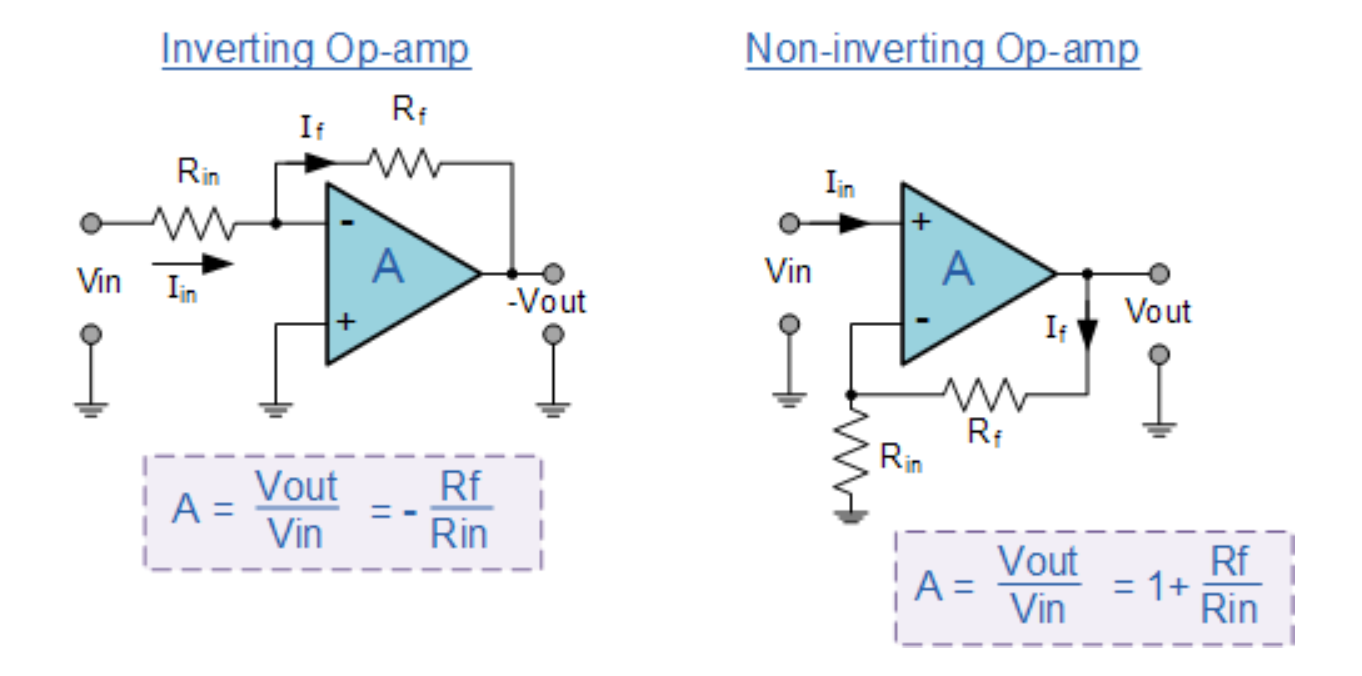
\includegraphics[width=0.70\textwidth]{graphics/invNoninv.png}
    \caption{Inverting and non inverting op amp setups \cite{noauthor_operational_2013}.}
    \label{fig:invNonInvOPamp}
\end{figure}

When the RC filter and op amps are combined, they form what is called an active filter.
Examples of which can be seen in \textit{Figures \ref{fig:LowPassFilter},\ref{fig:HighPassFiler}} and their respective frequency and phase shift responses in \textit{Figures \ref{fig:LowPassResponse},\ref{fig:HighPassResponse}}.
These filters performs the same as an RC filter in terms of its operations and frequency response with the addition of gain control \cite{noauthor_active_2013-1}.


\begin{equation}
    A_f = \frac{V{out}}{V{in}} = \frac{A_v}{\sqrt{1 + (\frac{f}{f_c})^2}}
    \label{eq:ActiveLowPass}
\end{equation}


The gain of the first order active low pass filter can be found using \textit{Equation \ref{eq:ActiveLowPass}}.
Where $A_f$ is the voltage gain, $A_v$ is the gain seen in \textit{Equation \ref{eq:DCGain}}, f is the frequency of the signal and $F_c$ is the set cutoff frequency.
This has the effect of active gain control depending on the frequency of the input.
When,
\begin{enumerate}
    \item $f < F_c$, $A_f \approx A_v$
    \item $f = F_c$, $A_f = \frac{A_v}{\sqrt{2}} = 0.707 A_v$
    \item$f > F_c$, $A_f < A_v$
\end{enumerate}

\begin{figure}[h]
    \centering
    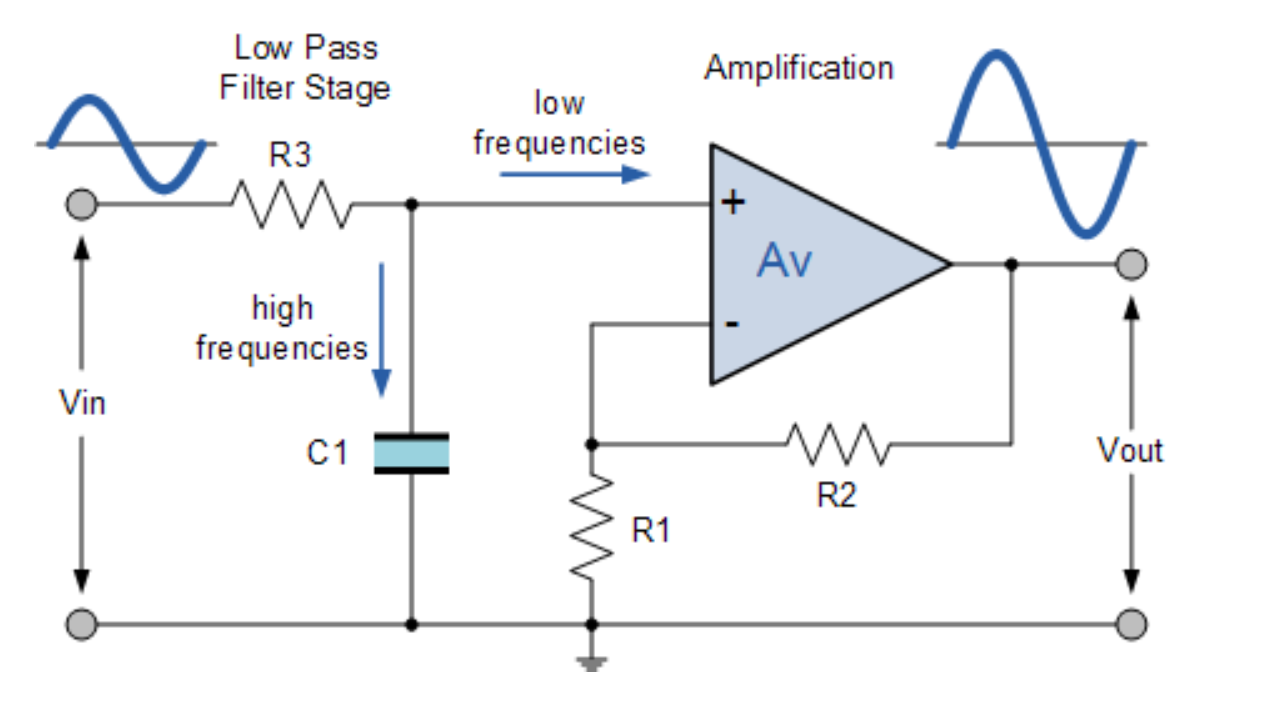
\includegraphics[width=0.70\textwidth]{graphics/lowPassFilter.png}
    \caption{Active first order low pass filter \cite{noauthor_active_2013-1}.}
    \label{fig:LowPassFilter}
\end{figure}

\begin{figure}[h]
    \centering
    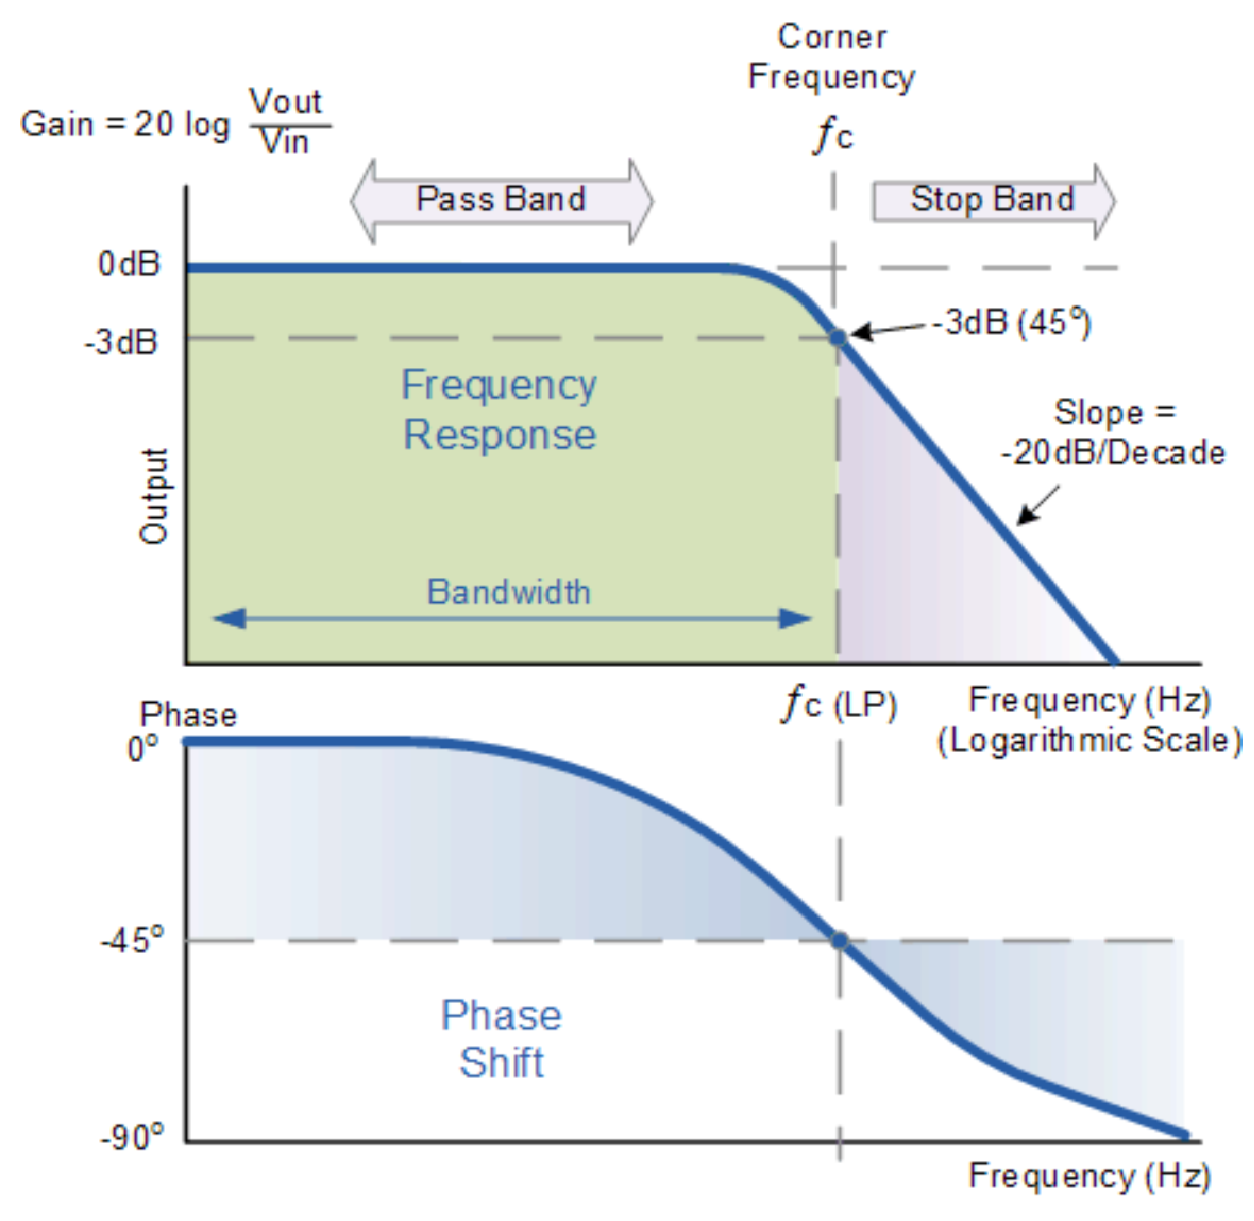
\includegraphics[width=0.70\textwidth]{graphics/lowPassResponse.png}
    \caption{First order RC low pass frequency response and phase shift \cite{noauthor_low_2013}}
    \label{fig:LowPassResponse}
\end{figure}


\begin{equation}
    A_f = \frac{V{out}}{V{in}} = \frac{A_v(\frac{f}{f_c})}{\sqrt{1 + (\frac{f}{f_c})^2}}
    \label{eq:ActiveHighPass}
\end{equation}

The gain of the first order active high pass filter can be found using \textit{Equation \ref{eq:ActiveHighPass}}.
Where $A_f$ is the voltage gain, $A_v$ is the gain seen in \textit{Equation \ref{eq:DCGain}}, f is the frequency of the signal and $F_c$ is the set cutoff frequency.
This has the effect of active gain control depending on the frequency of the input.
When,
\begin{enumerate}
    \item $f < F_c$, $A_f < A_v$
    \item $f = F_c$, $A_f = \frac{A_v}{\sqrt{2}} = 0.707 A_v$
    \item$f > F_c$, $A_f \approx A_v$
\end{enumerate}


\begin{figure}[h]
    \centering
    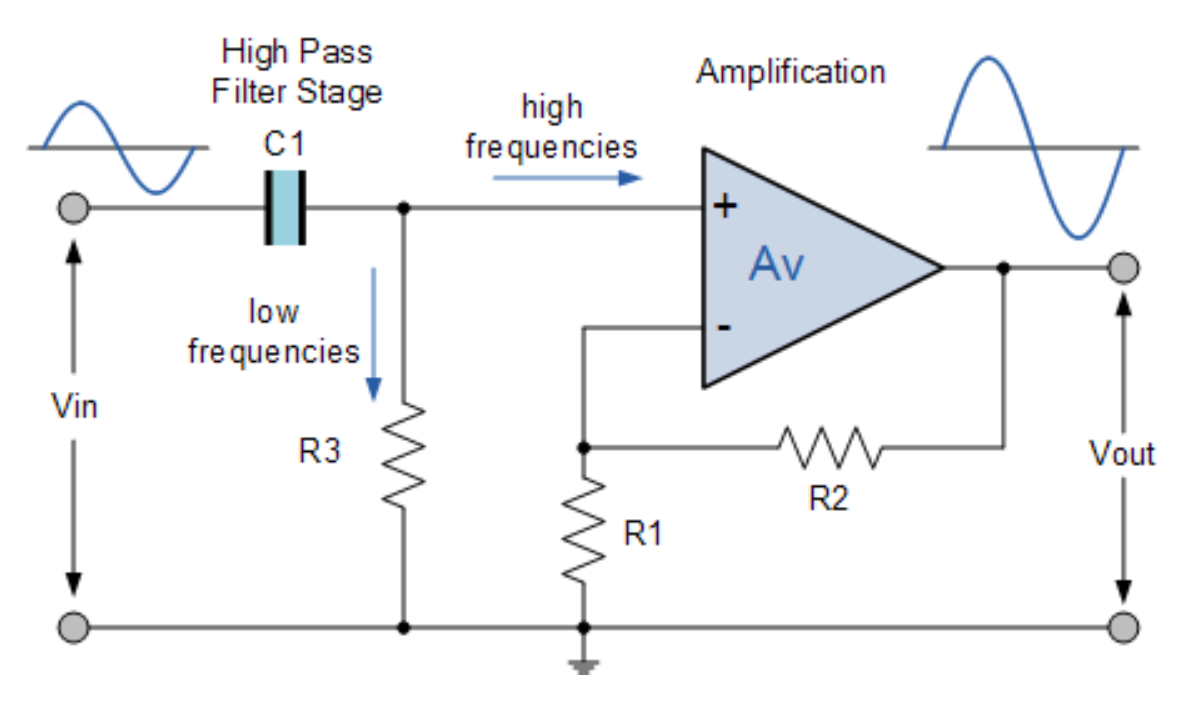
\includegraphics[width=0.60\textwidth]{graphics/highPassFilter.png}
    \caption{Active first order low pass filter \cite{noauthor_active_2013}.}
    \label{fig:HighPassFiler}
\end{figure}

\begin{figure}[h]
    \centering
    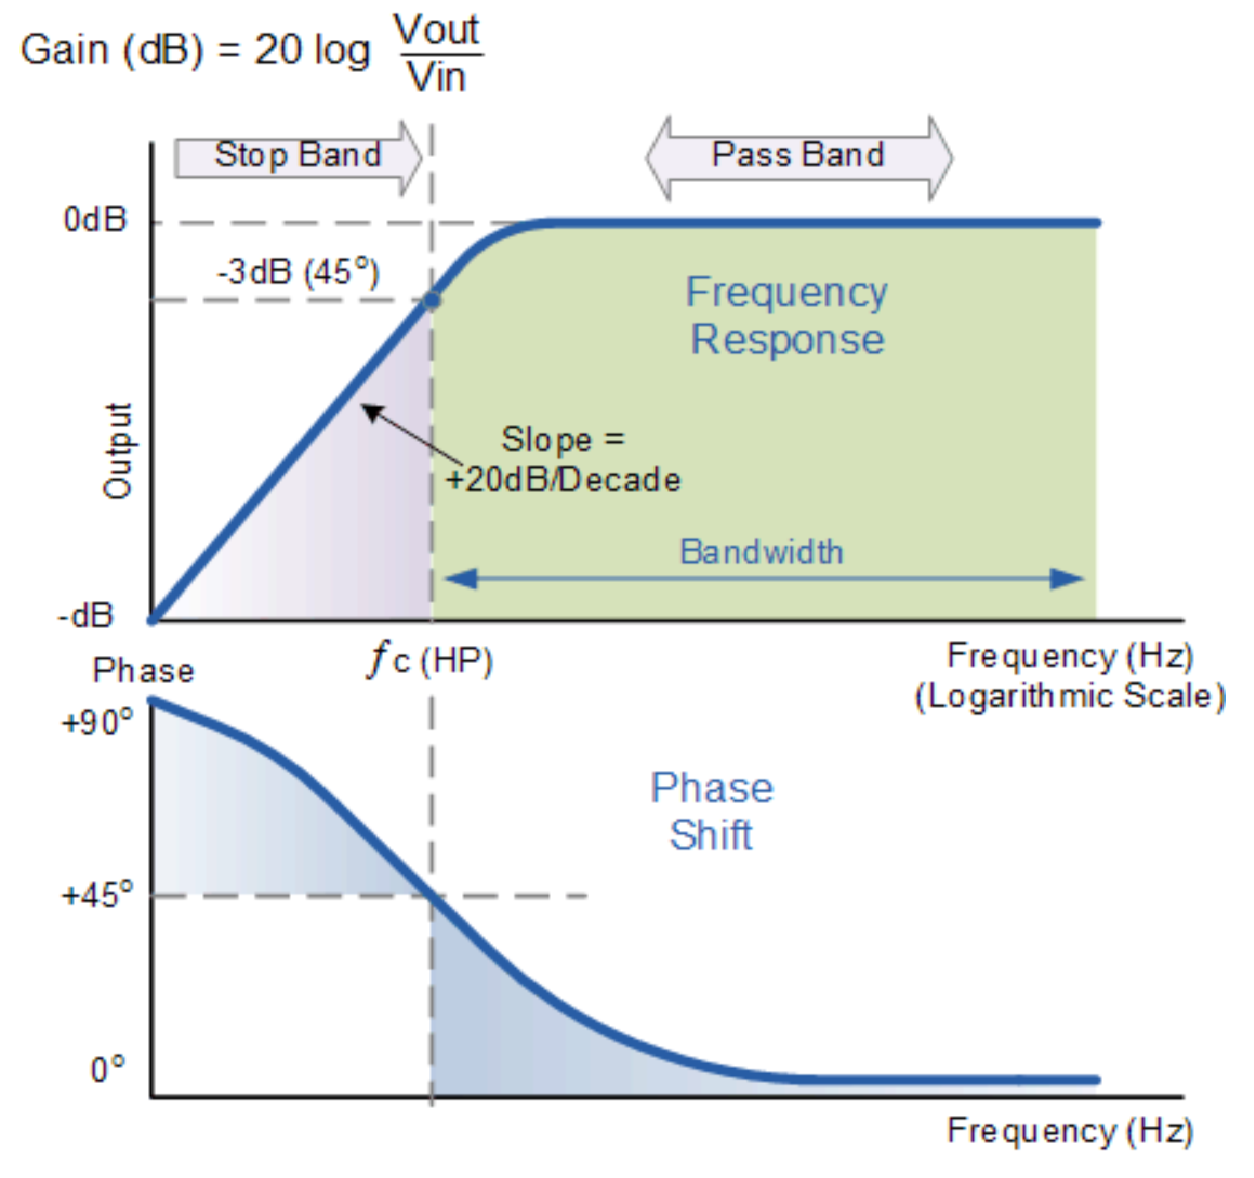
\includegraphics[width=0.60\textwidth]{graphics/highPassResponse.png}
    \caption{First order RC high pass frequency response and phase shift \cite{noauthor_high_2013}}
    \label{fig:HighPassResponse}
\end{figure}

\clearpage

Decibel is a relative unit of measure, used in electronic circuit to express the input values to output value on a logarithmic scale.  

\begin{equation}
    dB = 20log\frac{V{out}}{V{in}}
    \label{eq:DBGAIN}
\end{equation}

The gain in decibel is found by \textit{Equation \ref{eq:DBGAIN}}, where $V{out}$ is the output root mean square (rms) voltage of the circuit and V{in} is the input rms voltage.

Summing amplifiers or summing inverter circuits are useful when combining two or more signals together.
An example of the circuit can be seen in \textit{Figure \ref{fig:SummingOpAmp}}, where $R_1 = R_2 = R_3$ would be the same value.
The circuit yields a voltage output that is equal to all the input voltages summed together, multiplied with the unity gain of the amplifier.
This is possible due to the virtual ground that is created by a non inverting op amp configuration\cite{noauthor_summing_2013}. 
This circuit is especially useful when there is a need to shift an oscillating AC voltage to have a DC voltage offset.


\begin{figure}[h]
    \centering
    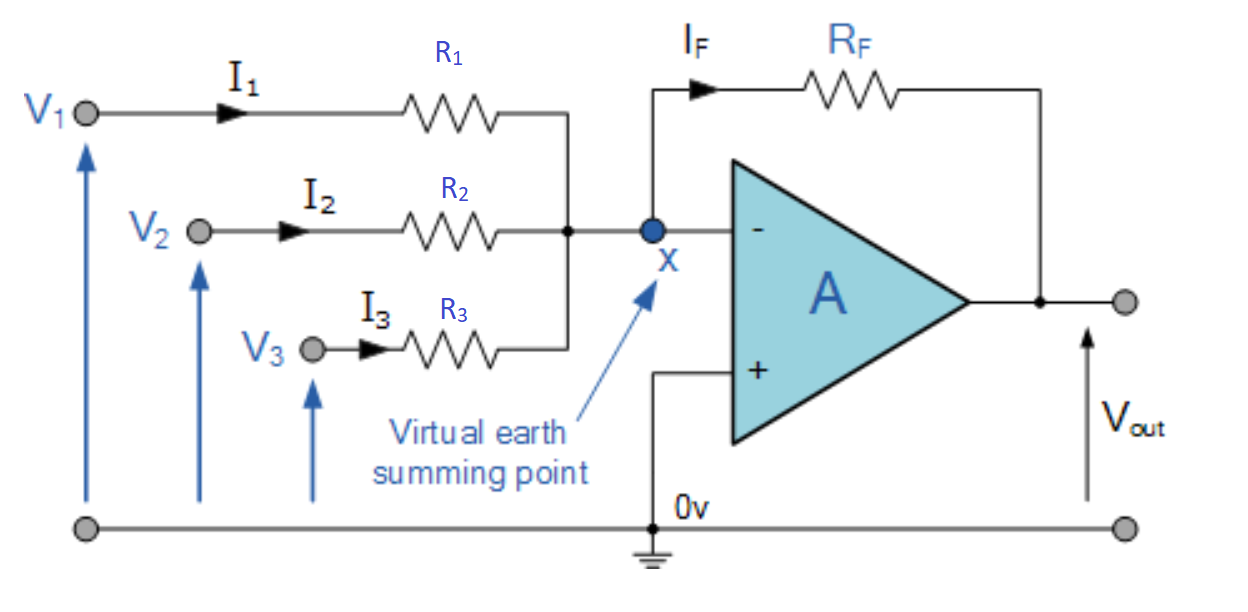
\includegraphics[width=0.70\textwidth]{graphics/SummingOpAmp.png}
    \caption{Scaling summing amplifier circuit \cite{noauthor_summing_2013}}
    \label{fig:SummingOpAmp}
\end{figure}

Scaling summing amplifiers are in the same configuration as summing amplifiers with one main difference which is that resistor values are not equal to one another.
This enables individual scaling of each signal, which means that each input signal can have different gain values.

%$$I_F = I_1 + I_2 + I_3 = -[\frac{V_1}{R_{1}} + \frac{V_2}{R_{2}} + \frac{V_3}{R_{3}}]$$
%$$-V_{out} = \frac{R_F}{R_{1}}V_1 +\frac{R_F}{R_{2}}V_2 +\frac{R_F}{R_{3}}V_3$$

\begin{equation}
    V_{out} = -R_F(\frac{V_1}{R_{1}} +\frac{V_2}{R_{2}} +\frac{V_3}{R_{3}} + ...)
    \label{eq:ScalingGain}
\end{equation}

Finding the output voltage can be found using \textit{Equation \ref{eq:ScalingGain}}.
Where $V_out$ is the output voltage, $R_f$ is the voltage across the input and output of the op amp, $R_1, R_2$ and $R_3$ are the resistor value of the different input signals.
Lets take for an example of an AC signal that needs to be shifted so that there is no negative voltage, see \textit{Figure \ref{fig:sumCircuitexamp}} for the layout of the circuit.
The AC signal (U1B\_out) would along with the shifting signal, in this case a DC voltage of 1.65V.
The AC signal is scaled by a factor of A = $\frac{180\Omega}{90\Omega}$ = 2.
How ever the DC voltage signal only scaled by a factor of A = $\frac{180\Omega}{180\Omega}$ = 1.
The voltage output, U1C\_out can be seen in \textit{Figure \ref{fig:SummingOpAmpShift}} as the red signal and the input signal, U1B\_out is represented by the white signal.
This creates a problem though, the output signal is shifted by $90\deg$ and the scaling op amp is in a inverting configuration the signal is inverted, so it is negative.
Both are fixed by the addition of U1D, an inverting amplifier.
Which puts the signal back in phase with the original input signal as well as it now is positive, as seen in \textit{Figure \ref{fig:SummingOpAmpShift1}} where the red signal is U1D\_out the output of the inverting amplifier and the white signal is the original input signal U1B\_out.


\begin{figure}[h]
    \centering
    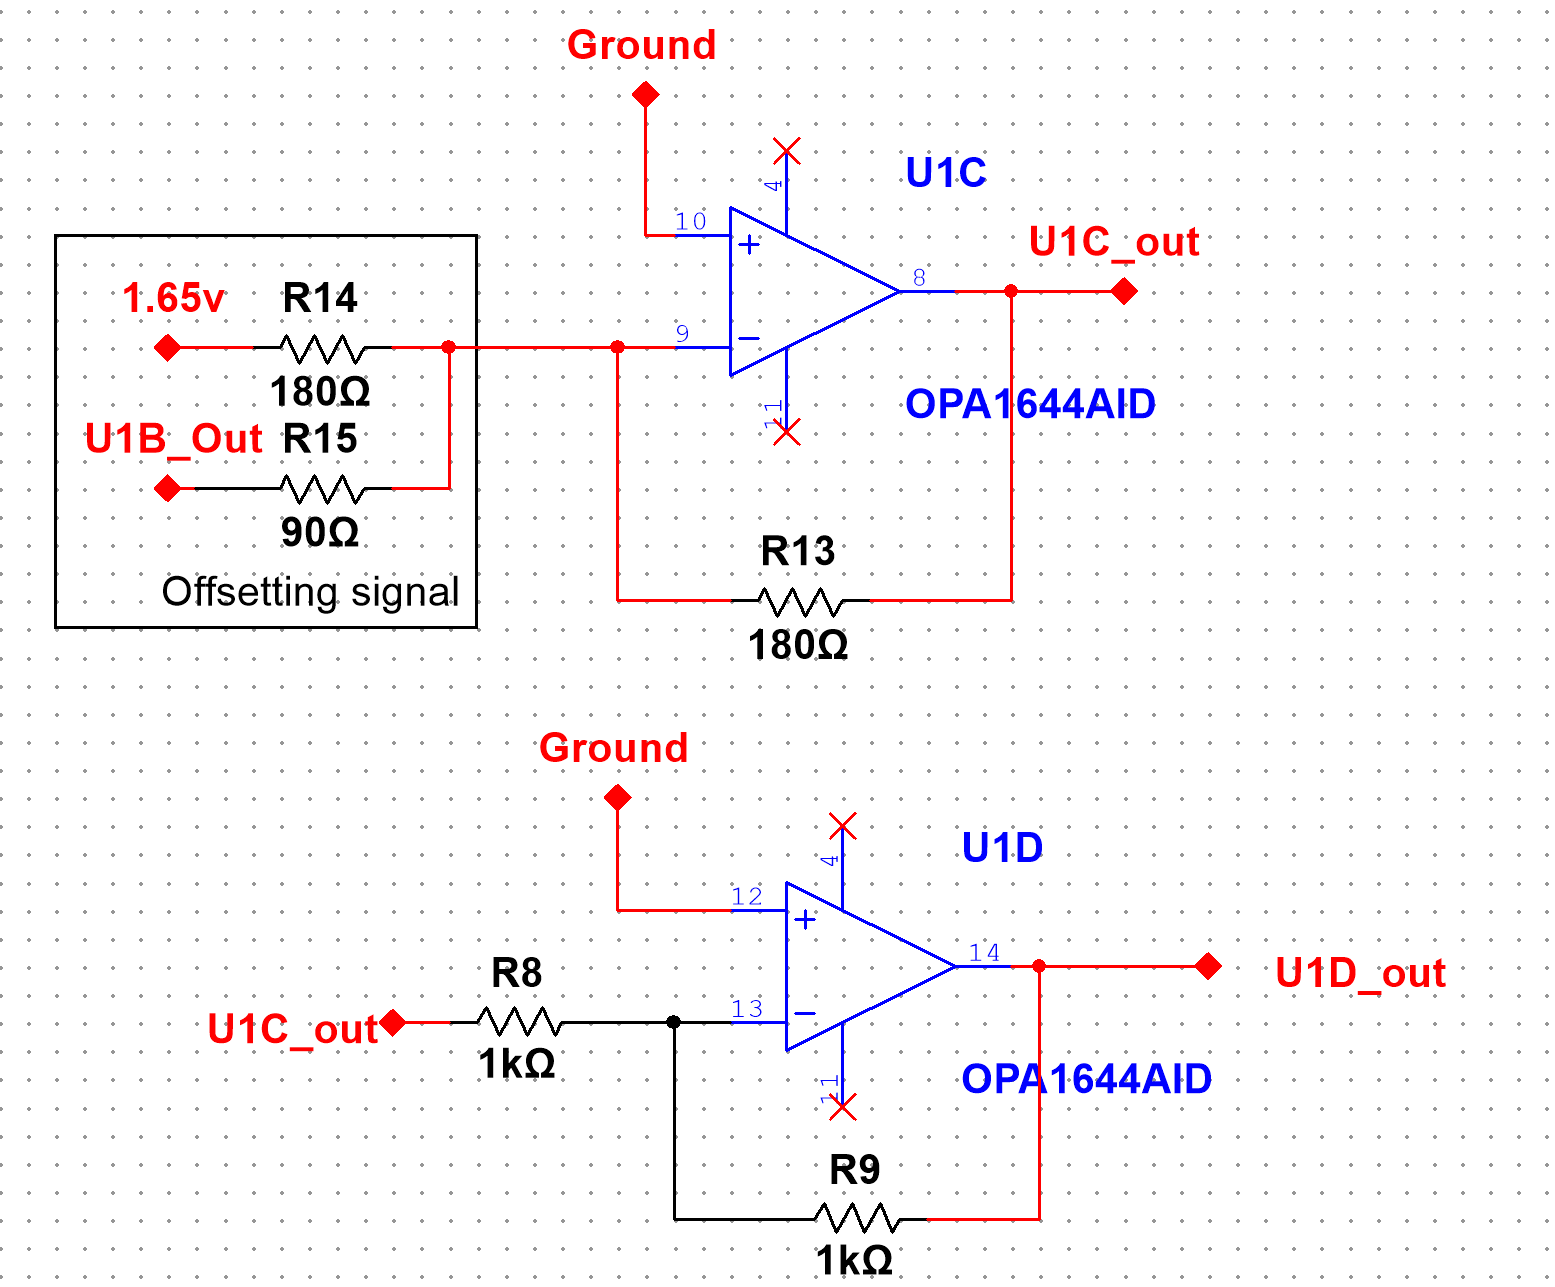
\includegraphics[width=0.70\textwidth]{graphics/sumCircuitexamp.png}
    \caption{Example of a scaling amplifier circuit where two signals are combined to create a shift of the original signal. U1C represents the scaling amplifier, U1D is a normal inverting amplifier.}
    \label{fig:sumCircuitexamp}
\end{figure}

\begin{figure}[h]
    \centering
    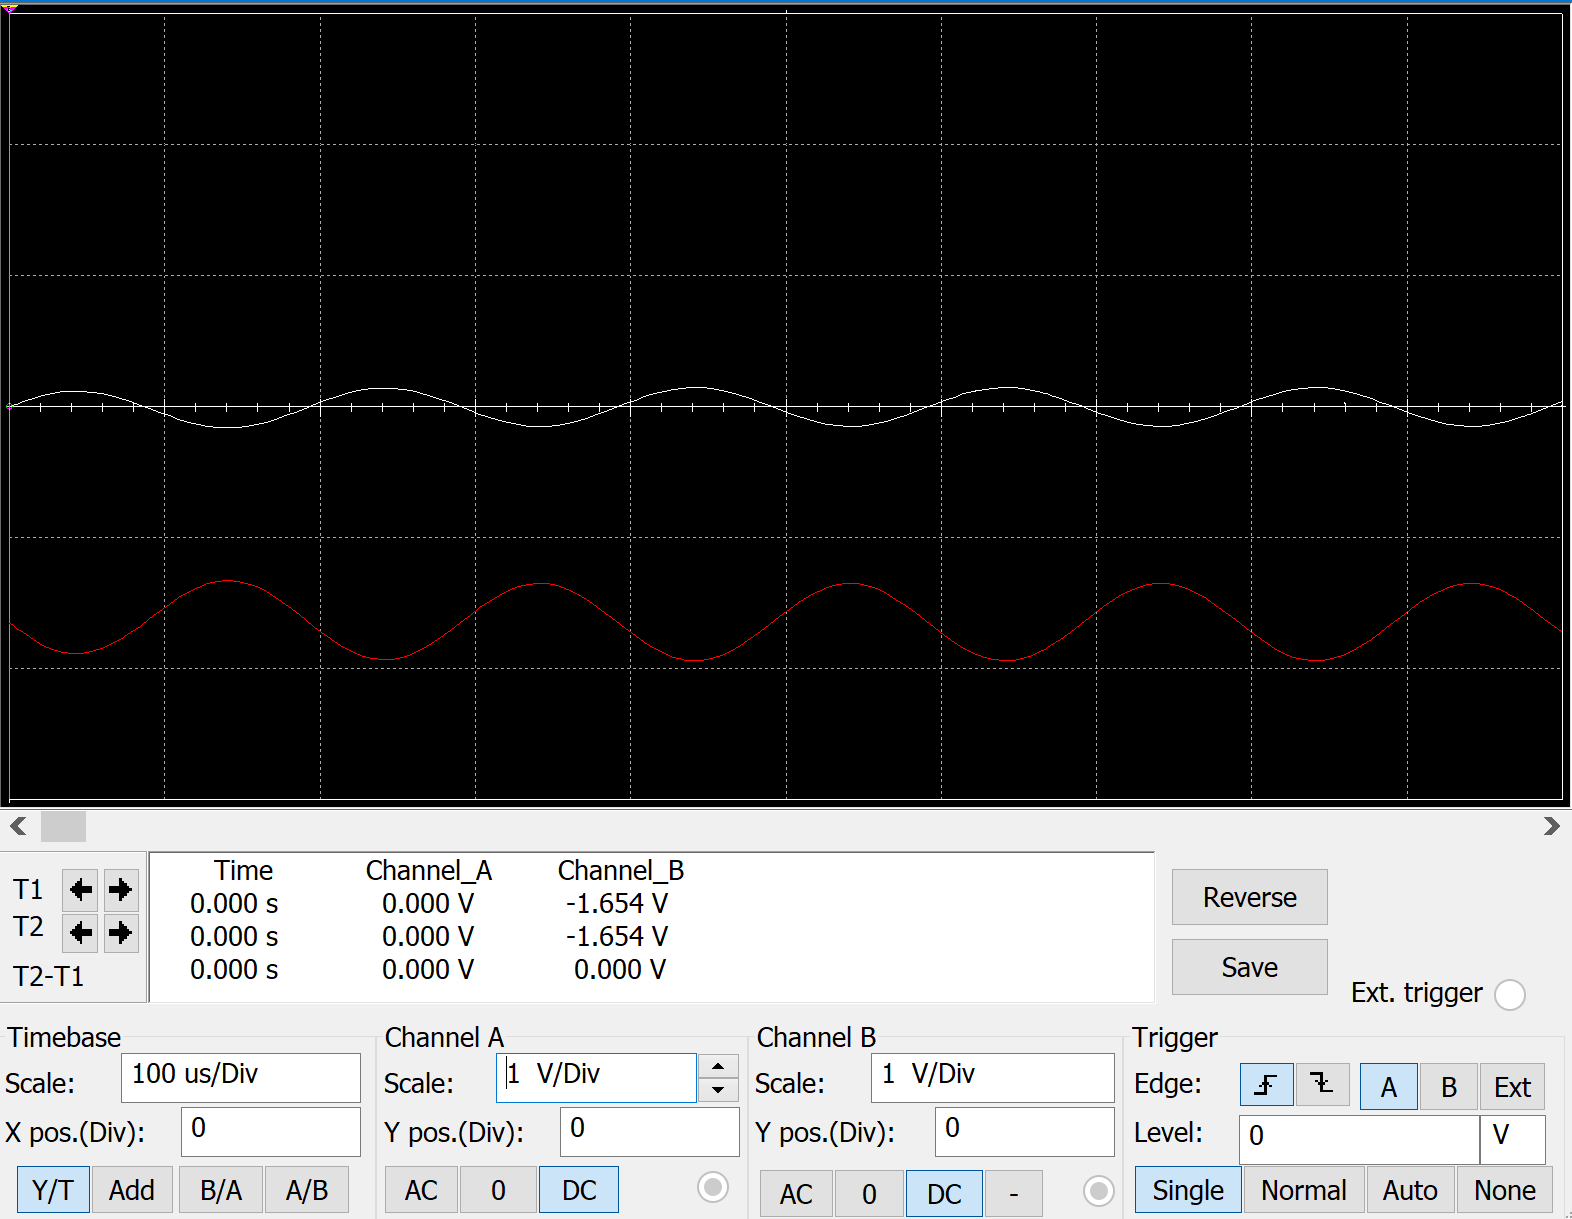
\includegraphics[width=0.70\textwidth]{graphics/summingShift.png}
    \caption{Example of the signal shift of a summing Op Amp circuit, the red signal represents the voltage output U1C\_out and the white signal is the input AC signal U1B\_out.}
    \label{fig:SummingOpAmpShift}
\end{figure}

\begin{figure}[h]
    \centering
    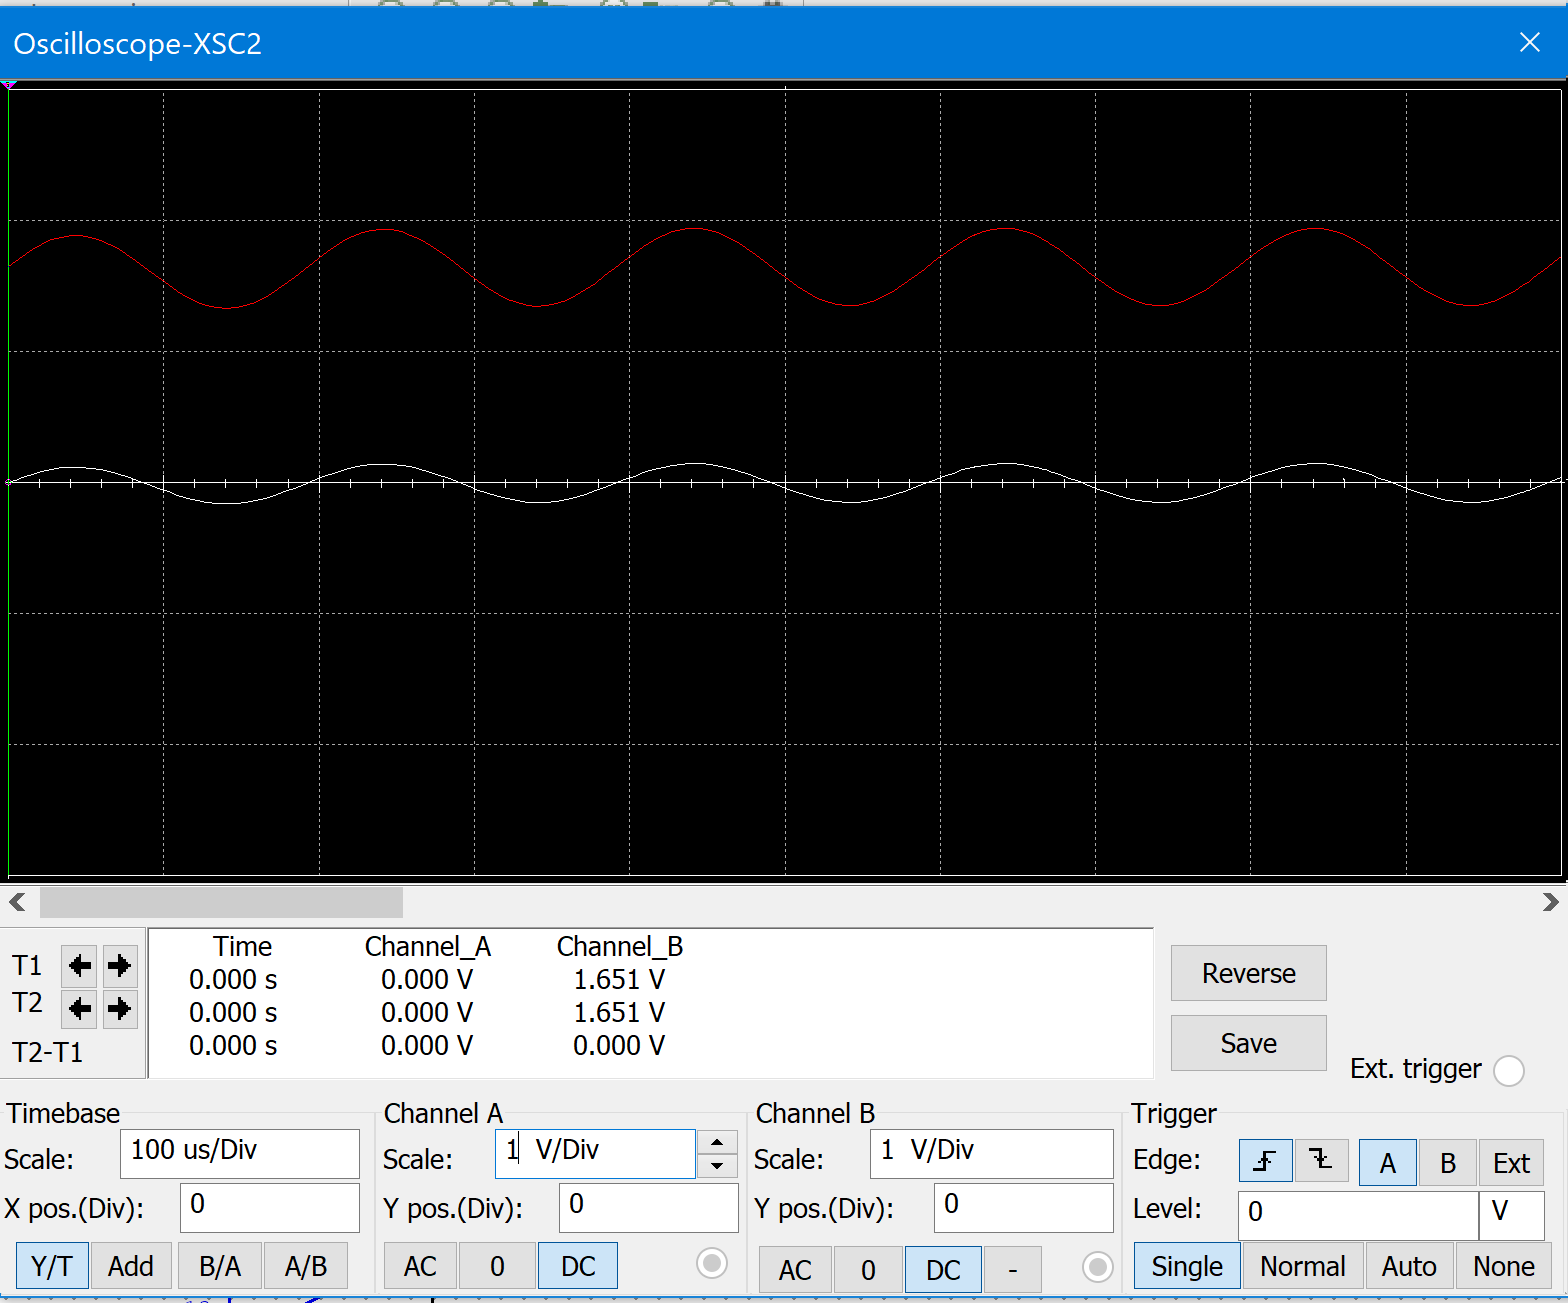
\includegraphics[width=0.70\textwidth]{graphics/summingShift1.png}
    \caption{Example of the signal shift of a summing Op Amp circuit, the red signal represents the voltage output U1D\_out and the white signal is the input AC signal U1B\_out}
    \label{fig:SummingOpAmpShift1}
\end{figure}


\clearpage

%\fxfatal{SKOÐA H'ER-----------------------}
%ADC CHARECTERISTICS https://forum.pjrc.com/threads/44929-Teensy-3-5-ADC-characteristcs
%SD POSSIBLE https://forum.pjrc.com/threads/45993-Teensy-3-6-ADC-DMA-Question
%Teensy36ISRLogger Skilar með 8gb kortinu 6.67MB/s
%https://forum.pjrc.com/threads/49975-writing-binary-file-on-SD-card-in-Teency-3-5

\subsection{Microcontroller/Microcomputer}%Breyta um titil

%For this project the most important factors when choosing a microcontroller/microcomputer were regarding the ADC specifications as well as the power consumption.%\fxfatal{VITNA Í GOALS} tala um upplausn bit, power og fleira

\subsubsection{Arduino}

Arduino Uno is a programmable board that uses the 8-bit ATmega328p microcontroller.
Which is probably one of the most popular microcontroller in the world and the Arduino board is one of the among the best beginner boards to use because of the shear amount of documentation and tutorials for it.
The microcontroller main features can be seen in \textit{Table \ref{Tab:ATmega328p}}.


\begin{figure}[h]
    \centering
    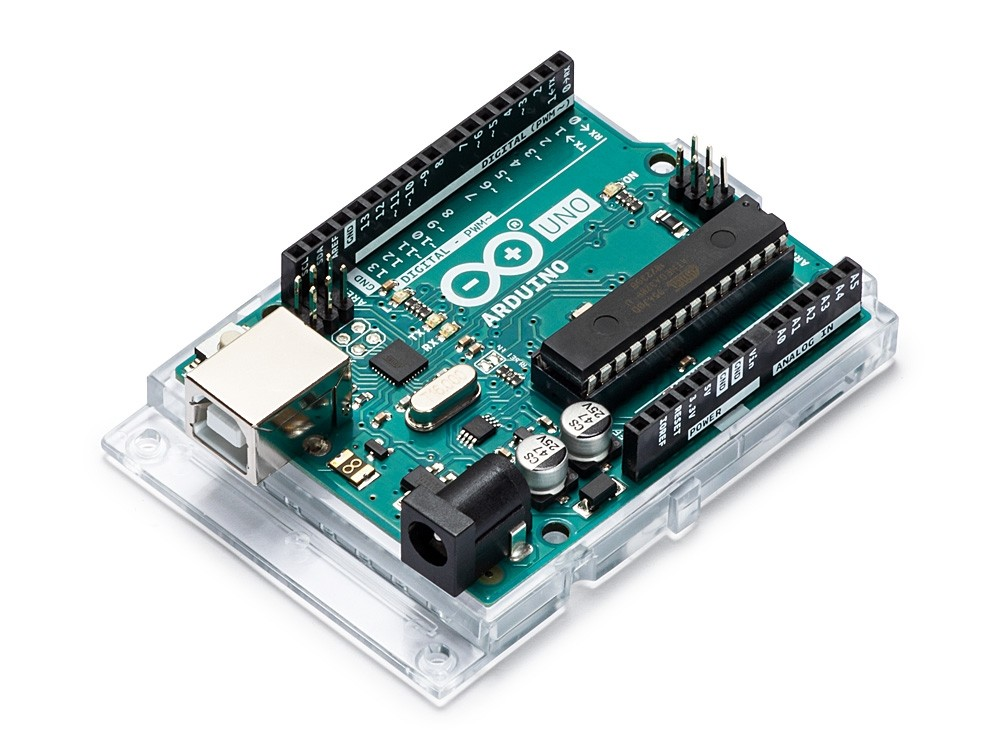
\includegraphics[width=0.70\textwidth]{graphics/ArduinoUNo.jpg}
    \caption{The Arduino Uno \cite{noauthor_arduino_nodate}}
    \label{fig:Arduino}
\end{figure}

\begin{table}[h]\caption{Main features of the ATmega328p \cite{noauthor_atmega328p_nodate}}.\label{Tab:ATmega328p}
\centering
    \begin{tabular}{|l|l|}
    \hline
        Parameters                        & Value                \\ \hline
        Flash memory [KB]                 & 32                      \\ \hline
        ADC resolution [bit]              & 10                   \\ \hline
        ADC sample speed [ksps]           & 15                     \\ \hline
        Digital Communication Peripherals & 1-UART, 2-SPI, 1-I2C \\ \hline
        Operating Voltage [V]             & 1.8 to 5.5           \\ \hline
        Max power consumption [W]         & 0.66               \\ \hline
        Price                             & 33\$                \\ \hline
    \end{tabular}
\end{table}


The Arduino has 14 digital input/output (I/O), and 6 can be used as pulse width modulation (PWM) outputs as well as 6 analog inputs.
The board has a USB connector which the board is programmed through as well as power it.
Arduino also provides its users with a free open source Arduino software integrated development environment (IDE).  \cite{noauthor_arduino_nodate}.
As well as a 6-channel 10-bit resolution ADC and up to 15 kilo samples per second (ksps) .
The board has a maximum current draw of 200mA, so at a operating voltage of 3.3V the power consumption is maximum 0.66W\cite{noauthor_atmega328p_nodate}.


\subsubsection{Raspberry Pi}

Unlike the Arduino the Raspberry Pi is not only a programmable microcontroller, but rather a single board microcomputer and is the third most sold computer brand worldwide \cite{noauthor_faqs_nodate}.
Currently there are 13 different model of the Raspberry Pi's with varying pricing and capabilities  some of which can be seen in \textit{Table \ref{Tab:RaspbModel}}. 
Raspberry Pis can be used with several operating system, for instance Linux, FreeBSD or a Raspberry pi OS that can come with or without a desktop.

\begin{center}
\begin{table}[h]\caption{Comparison of different Raspberry Pi models\cite{noauthor_faqs_nodate}}.\label{Tab:RaspbModel}
    \begin{tabular}{|l|l|l|l|c|}
    \hline
    \textbf{\begin{tabular}[c]{@{}l@{}}Raspberry Pi\\ Product\end{tabular}}        & \textbf{SoC} & \textbf{Speed} &  \textbf{\begin{tabular}[c]{@{}l@{}}Recommended\\ power supply \\ current capacity\end{tabular}} & \textbf{\begin{tabular}[c]{@{}l@{}}Typical bare-\\board current \\ consumption\end{tabular}} \\ \hline
     Model A+   & BCM2835      & 700MHz         & 0.7A          & 0.2A            \\ \hline
     Model B+   & BCM2835      & 700MHz         & 1.8A          & 0.33A            \\ \hline
     2 Model B  & BCM2836/7    & 900MHz         & 1.8A          & 0.5A                 \\ \hline
     3 Model B  & BCM2837A0/B0 & 1200MHz        & 2.5A          & 0.4A                  \\ \hline
     3 Model A+ & BCM2837B0    & 1400MHz        & 2.5A          & 0.35A                  \\ \hline
     3 Model B+ & BCM2837B0    & 1400MHz        & 2.5A          & 0.5A                  \\ \hline
     4 Model B  & BCM2711      & 1500MHz        & 3.0A          & 0.6A                  \\ \hline
     Zero       & BCM2835      & 1000MHz        & 1.2A          & 0.1A                   \\ \hline
     Zero W     & BCM2835      & 1000MHz        & 1.2A          & 0.15                  \\ \hline
     Zero WH    & BCM2835      & 1000MHz        & 1.2A          & 0.15                  \\ \hline
     400        & BCM2711      & 1800MHz        & 3.0A          & 0.8A                  \\ \hline
    \end{tabular}
\end{table}
\end{center}

Raspberry recommends powering the Raspberry Pi using 5V.
This means that the Raspberry Pi uses quite a bit of power,Raspberry Pi Zero (6W) Raspberry Pi 2 B (9W), Raspberry Pi 3(12.5W).
Taking a closer look at the Raspberry Pi Zero since it fits within the power consumption specifications.
The microcomputer costs around 30 \$, has a 1GHz single-core CPU, 512MB RAM, Mini HDMI port, Micro USB OTG port,
Micro USB power and HAT-compatible 40-pin header.
It has i2c, SPI, PWM and serial pins, all GPIO pins are digital and can be configured to be input or output pins.
which can be seen in \textit{Figure \ref{fig:RPIGPIO}}.

\begin{figure}[h]
    \centering
    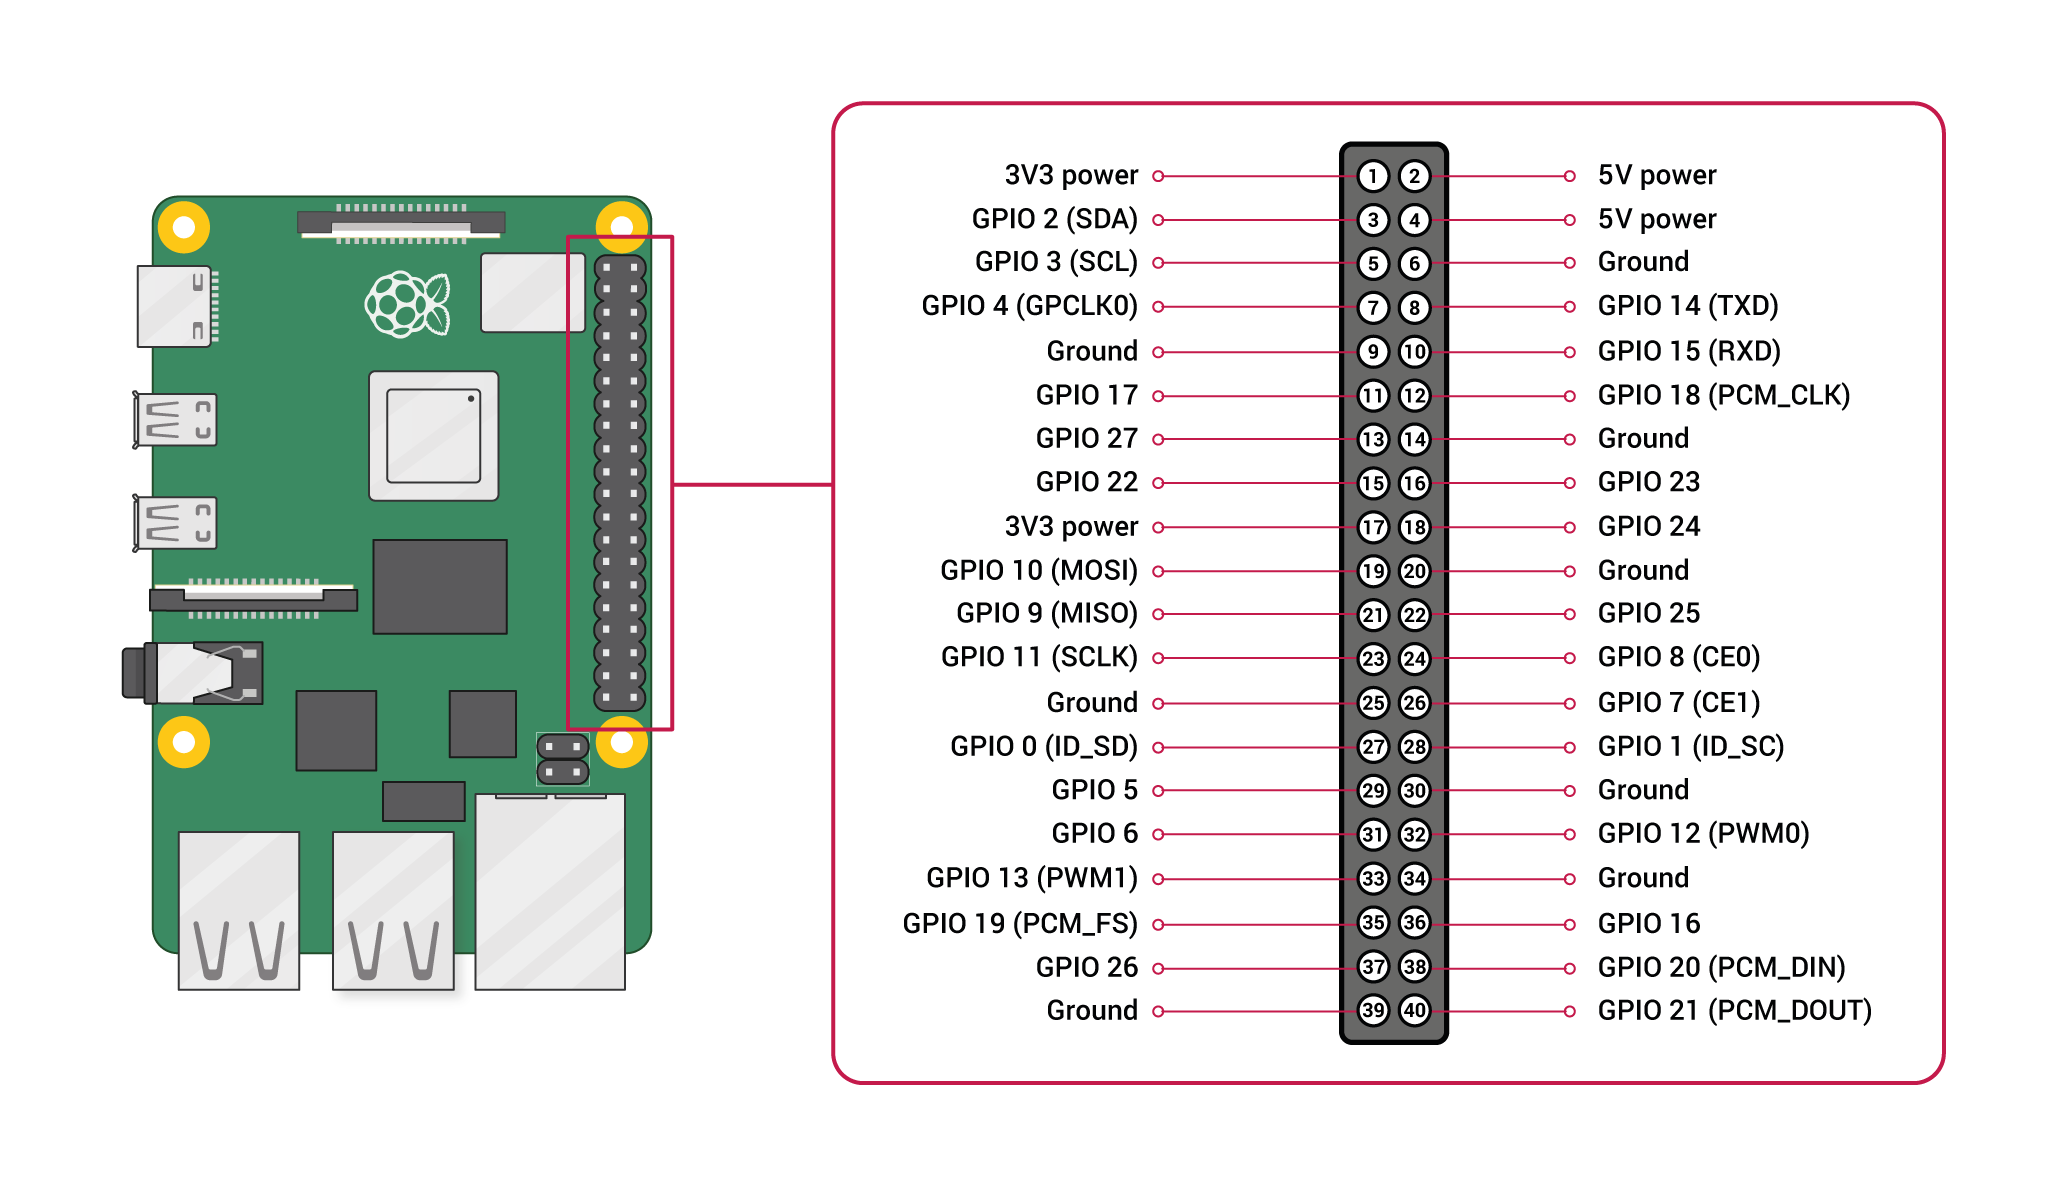
\includegraphics[width=0.70\textwidth]{graphics/ZeroGPIO.png}
    \caption{GPIO of the Raspberry Pi Zero \cite{noauthor_gpio_nodate}}
    \label{fig:RPIGPIO}
\end{figure}

The Raspberry Pi is also limited in the fact that it has no analog I/O pins, meaning that it can not convert analog to digital signal on its own.
However there is a way to record audio, which is done through sound card.
Several solutions have already been made available for this such as the Audio Injector stereo sound card which can directly connect to the general purpose input output (GPIO) pins of Raspberry Pi2, Pi3 and Pi Zero.
The card is made for an electret microphone and can supply the Raspberries with input and output audio.
The card has stereo RCA input and output, a headphone jack and a preamplifier, a volume knob and a low latency of 540 $\mu$s for both the input and output \cite{noauthor_rpi_nodate}.

\begin{figure}[h]
    \centering
    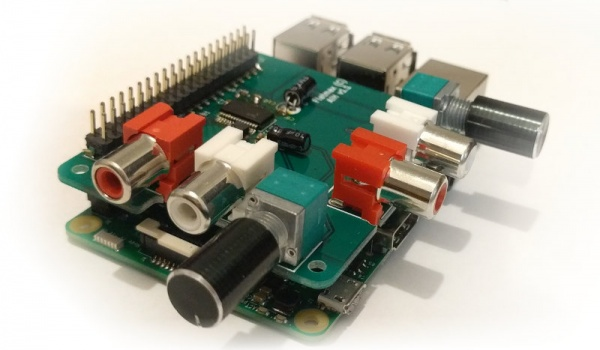
\includegraphics[width=0.70\textwidth]{graphics/rpisoundcard.jpg}
    \caption{The Audio Injector stereo sound card \cite{noauthor_rpi_nodate}}
    \label{fig:rpisoundcard}
\end{figure}


\subsubsection{Teensy}

Teensy's are the same as Arduino as being a USB programmable single board microcontroller.
The boards are can be programmed with multiple of programs such as the Arduino IDE software and can use both the examples and libraries that come with the program.
This is possible through an addition called Teensyduino which also includes a large library for programming.
Other programs include Visual Micro, which enables programming on Visual Studio Code, PlaformIO IDE and CircuitPython (only available on Teensy 4.X) which allows python programming.
There are multiple models available, ranging in price, size and capabilities as seen in \textit{Table \ref{Tab:TeensyModel}}.


\begin{table}[h]\caption{Comparison of different Teensy models\cite{noauthor_teensy_nodate}}.\label{Tab:TeensyModel}
\begin{tabular}{|l|l|l|l|l|}
\hline
\multicolumn{1}{|c|}{\textbf{Specification}} & \multicolumn{1}{c|}{\textbf{Teensy 2.0}}                               & \multicolumn{1}{c|}{\textbf{Teensy 3.0}}                                            & \multicolumn{1}{c|}{\textbf{Teensy 3.5}}                                                  & \multicolumn{1}{c|}{\textbf{Teensy 4.1}}                                              \\ \hline
Processor & \begin{tabular}[c]{@{}l@{}}ATMEGA32U4\\ 8 bit AVR\\ 16 MHz\end{tabular} & \begin{tabular}[c]{@{}l@{}}MK20DX128\\ 32 bit ARM\\ Cortex-M4\\ 48 MHz\end{tabular} & \begin{tabular}[c]{@{}l@{}}MK64FX51\\2VMD12\\ 32-bit ARM\\ Cortex- M4\\ 120MHz\end{tabular} & \begin{tabular}[c]{@{}l@{}}MIMXRT1062\\ 32 bit ARM\\ Cortex-M7\\ 600 MHz\end{tabular} \\ \hline
\begin{tabular}[c]{@{}l@{}}Flash Memory\\ {[KB]}\end{tabular} & 32 & 131 & 512 & 7936 \\ \hline
%\begin{tabular}[c]{@{}l@{}}RAM Memory\\ (Bytes)\end{tabular}& 2560 & 16384 & 256K & 1024K \\ \hline
%\begin{tabular}[c]{@{}l@{}}EEPROM\\ (Bytes)\end{tabular} & 1024 & 2048 & 4096 & 4096 \\ \hline
\begin{tabular}[c]{@{}l@{}}Direct Memory\\ Access [Channels]\end{tabular}  & - & 16 & 16 & 32 \\ \hline
%I/O [Pins, V] & 25, 5 Volt & 34, 3.3 V & \begin{tabular}[c]{@{}l@{}}64, 3.3V,\\ 5V tol\end{tabular} &\begin{tabular}[c]{@{}l@{}}55, 3.3V,\\ 5V tol\end{tabular}   \\ \hline
\begin{tabular}[c]{@{}l@{}}ADC resolution\\ {[bit]}\end{tabular} & 10 & 16 & 16   & 12     \\ \hline
%PWM & 7 & 10 & 20 & 35 \\ \hline
UART,I2C,SPI & 1,1,1 & 3,1,1 & 6,3,3 & 8,3,3 \\ \hline
Price [\$] & {16.00} & {19.00} & {24.25} & {26.85} \\ \hline
\end{tabular}
\end{table}

Taking a closer look at the comparison between the Teensy 3.5 and Teensy 4.1.
Teensy 3.5 has 2 16bit, 416 ksps (in 16 bit mode) and 818.3 ksps for (<= 13 bit mode), 12MHz ADC\cite{freescale_semiconductor_kinetis_2021-1} and has a voltage range of 0-3.3V as well as some are 5V tolerant while the Teensy 4.1 offers 12 bits of resolution and 20MHz (samples per second is not specified) and a range of 0 - 3.3V.
%The Teensy 3.5 also has an option of using pins connected to differential amplifiers, which can decrease unwanted noise of input analog signals.
%Teensy 3.5 also has two Digital to analog converters (DACs) output.
%Which makes it capable of outputting audio signals.
Both Teensys have a voltage regulator which reduces the 5V VUSB / VIN power to 3.3V for use by the main processor and most other parts. Additional circuitry may be powered from the 3.3V pin.
The recommended maximum for external 3.3V usage is 250mA or 0.825W.
When Teensy 3.5 is running at 120MHz processor speed it consumes roughly 50mA at 5V or 0.25W.
While the Teensy 4.0 consumes roughly 100mA at 5V or 0.5W at 600MHz processor speed.
%When power is not applied to VUSB or VIN, it is however possible to run by externally applying 3.3V power.
%There are two ways to power the Teensy's, the first one is to power them via USB.
%The Teensys are equipped with a voltage regulator which regulates the USB voltage of 5V down to 3.3V.
%They can also be powered straight to a VIN pin, which is recommended as a maximum of 3.3V and a 250mA %draw.
\cite{noauthor_teensy_nodate-1}%4.1
\cite{noauthor_teensy_nodate-2}.%3.5

%%% Local Variables: 
%%% mode: latex
%%% TeX-master: "DEGREE-NAME-YEAR"
%%% End: 
%%RUM: Introduction
\chapter{Methods}

\section{Cetacean vocalization}

Many species of cetaceans can be found near Iceland.
There are at least 12 species of cetaceans that roam Icelands waters.
Among which are most frequently spotted are harbour porpoise, white beaked dolphins, minke whales and humpback whales \cite{user_whales_nodate}.
Sound is used by cetaceans for various purposes such as communication, prey hunting, predator avoidance as well as navigation \cite{nowacek_studying_2016}.
Each species can vocalize different sounds.
The sounds can be described as moans, calls, clicks, shrieks and more.
Cetaceans use these sounds to low frequency sound for communicating to one another all the way to creating high frequencies echolocation sounds for hunting their prey\cite{greenhow_hearing_nodate}.
Table \ref{Tab:WhaleHz} shows the type of sound, frequency range of the sound, the dominant frequency of the sound and the source level of each sound for its respective species.

\newpage


\begin{table}[]\caption{Frequency ranges of whales that are found near Iceland \cite{richardson_marine_2013}}.\label{Tab:WhaleHz}
\centering
\resizebox{\textwidth}{!}{
\begin{tabular}{|l|l|l|l|l|}
\hline
\begin{tabular}[c]{@{}l@{}}Species \\ of \\ whale\end{tabular} & Noise type             & \begin{tabular}[c]{@{}l@{}}Frequency range\\ {[}Hz{]}\end{tabular} & \begin{tabular}[c]{@{}l@{}}Dominant \\ frequencies \\ {[}Hz{]}\end{tabular} & \begin{tabular}[c]{@{}l@{}}Source level \\ {[}dB re 1 $\mu$Pa at 1m{]}\end{tabular} \\ \hline
Blue    & Moans & 12 - 390 & 16 - 26 & 188 \\ \cline{2-5}
        & Clicks & \begin{tabular}[c]{@{}l@{}}  6k - 8k\\ 21k - 31k\end{tabular} & \begin{tabular}[c]{@{}l@{}}6k - 8k\\ 25k\end{tabular} & \begin{tabular}[c]{@{}l@{}}130\\ 159\end{tabular} \\ \hline
\begin{tabular}[c]{@{}l@{}}Bottlenose \\dolphin\end{tabular}    & Whistles & 0.8 - 24 & 4.5 - 14.5 & 125 - 173 \\ \cline{2-5}
        & \begin{tabular}[c]{@{}l@{}}Low-freq. \\narrowband\end{tabular}    & < 2 & 0.3 - 0.9 & - \\ \hline
Fin     & Moans, down sweeps & 14 - 118 & 20 & 160 - 186 \\ \cline{2-5}
        & Constant call & 20 - 40 & - & - \\ \cline{2-5}
        & Moans, tones, up sweeps & 30 - 750 & - & 155 - 165 \\ \cline{2-5}
        & Rumble & 10 - 30 & - & - \\ \cline{2-5}
        & Whistles, chirps & 1.5k - 5k & 1.5k - 2.5k & - \\ \cline{2-5}
        & Clicks & 16k - 28k & - & - \\ \hline
Harbour porpoises & Clicks & 2 & - & 100 \\ \cline{2-5}
        & Echolocation & 110k - 150k & - & 135 - 177 \\ \hline
Humpback & Song components & 30 - 8k & 120 - 4k & 144 - 174 \\ \cline{2-5}
        & Shrieks & - & 750 - 1.8k & 179 - 181 \\\cline{2-5}
        & Horn blasts & - & 410 - 420 & 181 - 185 \\ \cline{2-5}
        & Moans & 20 - 1.8k & 35 - 360 & 175 \\\cline{2-5}
        & Grunts & 50 - 1.9k+ & - & 190 \\\cline{2-5}
        & Pules trains & 25 - 1.25k & 25 - 80 & 179-181 \\ \cline{2-5}
        & Underwater blows & 100 - 2k & - & 158 \\\cline{2-5}
        & Fluke and flipper slap & 30 - 1.2k & - & 183-192 \\\cline{2-5}
        & Clicks & 2k - 8.2k & - & - \\ \hline
Minke & Down sweeps & 60 - 130 & - & 165 \\ \cline{2-5}
        & Moans, grunts & 60 - 140 & 60 - 140 & 151 - 175 \\\cline{2-5}
        & Ratchet & 850 - 6k & 850 & - \\ \cline{2-5}
        & Clicks & 3.3k - 20k & \textless{}12k & 151 \\ \cline{2-5}
        & Thump trains & 100 - 2k & 100 - 200 & - \\ \hline
Killer  & Whistles & 1.5k - 18k & 6k - 12k & - \\ \cline{2-5}
        & Pulsed calls & 500 - 25k & 1k - 6k & 160 \\ \cline{2-5}
        & Echolocation & 12k - 25k & - & 180 \\ \hline
Sei     & FM sweeps & 1.5k - 3.5k & - & - \\ \hline
Sperm    & Clicks & 0.1 - 30 & 2 - 4, 10 - 16 & 160 - 180 \\ \hline
\begin{tabular}[c]{@{}l@{}}White-beaked\\dolphin\end{tabular} & Squeals & - & 8 - 12 & - \\ \hline

\end{tabular}}
\end{table}

Cetaceans creature produce sounds with a wide bandwidth, or 2 - 150k Hz as seen in \textit{Table \ref{Tab:WhaleHz}}.
In comparison humans have vocalization range of up to 5kHz and a hearing range from 16Hz - 20kHz \cite{monson_perceptual_2014}.
The vocalization is so powerful that the low frequency sounds can travel thousands of kilometers\cite{nowacek_studying_2016}.
The energy of sounds from for example killer whales, in calm seas that the sound can travel up to 25.9km.\cite{miller_diversity_2006}.

\newpage

\subsection{Audio}

\subsubsection{Sound wave}

Sound is a mechanical vibration, which results in an oscillating wave.
The wave causes a change in pressure of molecules 
The wave can travel through gasses, liquids and solids.
It occurs when objects vibrate such as a diaphragm of a speaker or a vocal cord of a human.
It is a wave that has a frequency and amplitude, which determines the type of sound and the intensity of the sound.
Sound waves behave very differently in liquid and in air.
In liquid such as sea water there are several things that affect sound propagation.
Such as the waves can bounce off particles or other sea creature. 
The bottom of the sea and the surface reflect waves and cause energy.
Finally and the largest factor  is depth, salinity and temperature of the water .
These factors can distort the sound and create transmission loss\cite{noauthor_sonar_nodate}.


\begin{figure}[h]
    \centering
    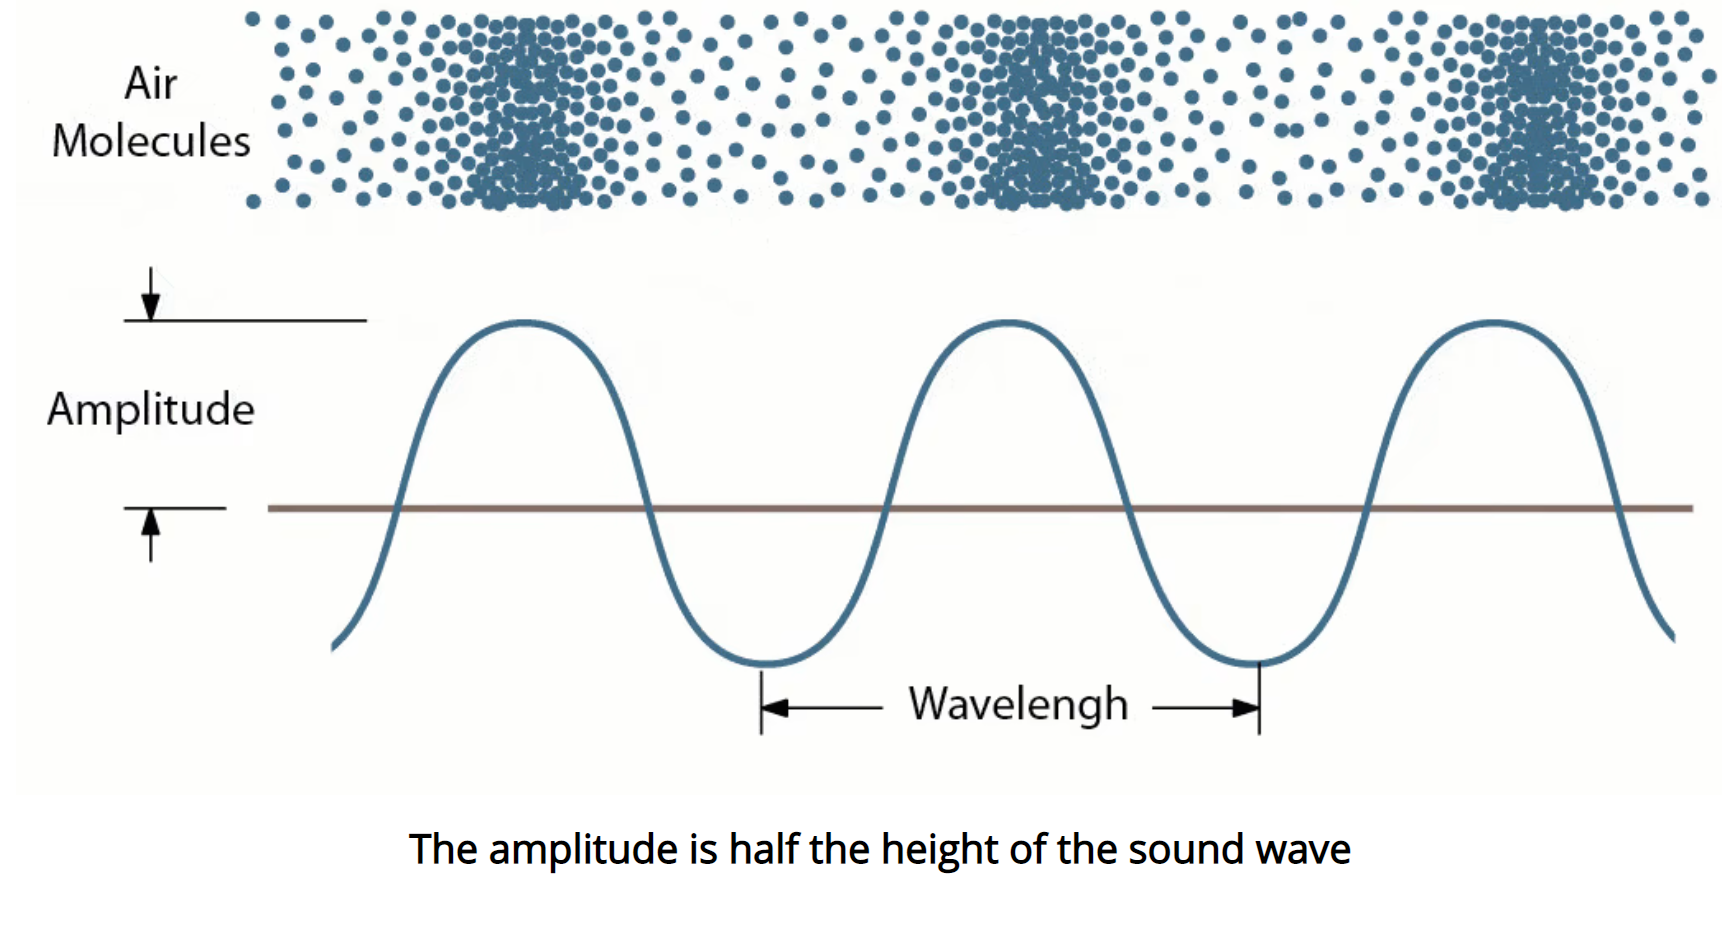
\includegraphics[width=0.70\textwidth]{graphics/soundwaves.png}
    \caption{How molecules react to sound waves \cite{noauthor_what_nodate}}
    \label{fig:SoundWaves}
\end{figure}

\subsubsection{Audio recording}

\fxfatal{MÖGULEGA BÆTA VIð TALA UM\\ RESOLUTION OG SÖFNUNART'IÐNI td og Nyquist}




\section{Device hardware}







\textbf{FARA 'I GEGNUM VERKEFNI SEM AÐRIR HAFA GERT RUNNA ÞAU OG TALA UM NIÐURSTÖÐUR OG DÆMA HVÐ VIRKAR HVAÐ EKKI OG AFHVERJU ÞETTA GETUR VERIÐ EH APPENDIX DÆMI
}









\subsection{Hydrophone}

Hydrophones are devices specially designed for underwater sound recording.
One of the earliest known examples of a hydrophone was made by stretching a membrane tightly over the end of a tube, one end of the tube is placed underwater while the other end is placed to the observers ear \cite{wood_a_b_textbook_1946}. 
Modern hydrophone are mainly based on piezoelectric transducers.
These hydrophones have been used since the early stages of world war 1.
Paul Langevin developed the first piezoelectric hydrophone, which was intended to be used for the detection of submarines.
A vacuum tube amplifier in combination with a piezoelectric material to be used as a transducer signal\cite{van_der_kloot_great_2014}.

When choosing a hydrophone it is important to look at a few specifications in the data sheet of the hydrophone. 
Such as the open circuit receiving response (OCRR), which is what the transducer outputs in terms of dB re 1V/$\mu$Pa.
Which is function of frequency and expressed in terms of dB re 1V/$\mu$Pa.
Sound intensity level (SIL) is the intensity of the sound at the transducer and is expressed in terms of dB re $\mu$Pa.
Transmitting voltage response (TVR) is the output voltage of the SIL at 1m range from the transducer and is expressed in terms of dB re $\mu$Pa/1V @ 1m \cite{ethem_mutlu_sozer_underwater_nodate}. 
Usable frequency of the hydrophone, directional patterns of the hydrophone and if the it applies the nominal capacitance of the hydrophone are also important factors. 
If for example the CRT C57 hydrophone was chosen, specifications can be seen in \textit{Table \ref{Tab:CRT57Hydrip}}.

\newpage

\begin{table}[h]\caption{Specifications of CRT C57 hydrophone range \cite{computing_c57_nodate}}.\label{Tab:CRT57Hydrip}
\centering
\begin{tabular}{|r|c|c|}
\hline
\multicolumn{1}{|c|}{\textbf{}} & C57 / C57X & C57RS/C57XRS \\\hline
{\begin{tabular}[c]{@{}r@{}}Linear Frequency Range \\ (±3dB) {[}kHz{]}\end{tabular}}      & 0.015 to 45         & \begin{tabular}[c]{@{}c@{}}0.015 to 50\&\\ 124 to 250+\end{tabular} \\ \hline
{\begin{tabular}[c]{@{}r@{}}Usable Frequency Range \\ (+3/-12dB) {[}kHz{]}\end{tabular}}  & 0.008 to 100        & { 0.008 to 77 \& 96 to 250+}                    \\ \hline
{\begin{tabular}[c]{@{}r@{}}Transducer Sensitivity* \\ {[}dB, re 1V/µPa{]}\end{tabular}}  & -187                & { -200}                                         \\ \hline
{Preamplifier Gain {[}dB{]}}                   & 20 / 33             & { 20 / 33}                                      \\ \hline
{\begin{tabular}[c]{@{}r@{}}Effective Sensitivity*\\  {[}dB, re 1V/µPa{]}\end{tabular}}   & -167 / -154         & { -180 / -167}  \\  \hline
\multicolumn{1}{|l|}{\begin{tabular}[c]{@{}l@{}}Price from dealer \\ {[}€{]}\end{tabular}} & \multicolumn{1}{|l|}{1290/1290} & \multicolumn{1}{|l|}{1290/1290} \\ \hline
\end{tabular}
\end{table}

If the CRT C57RS was chosen, which has an OCRR of -200 db re 1V/$\mu$Pa over a frequency range of 0.008 to 77kHz. 
Lets say a Blue whale is producing a moan which from \textit{Table \ref{Tab:WhaleHz}} indicates that the SIL would be 188dB re $\mu$Pa.
Then $VdB = SIL + OCRR = 188 + (-200) = -12dB$.
Because VdB is relative to 1V, the voltage output can be described as $V = 10^{VdB/10}$
which means the voltage output of the hydrophone would then be $V = 10^{-12dB/10} = 63mV$.

% Converting the oscillating mechanical pressure difference (sound waves) to electrical energy \cite{li_piezoelectric_2012}.
% https://www.researchgate.net/publication/255001750_Piezoelectric_Materials_Used_in_Underwater_Acoustic_Transducers
% https://archive.org/details/in.ernet.dli.2015.15768/page/n471/mode/2up
% https://en.wikipedia.org/wiki/Hydrophone#cite_note-3
%https://se.mathworks.com/help/phased/ref/phased.isotropichydrophone-system-object.html

\subsection{Signal conditioning}

Conditioning the output signal produced by the hydrophone is important in order to only monitor desired values.
Unwanted frequencies need to be filtered out in order to get a cleaner signal in the range that is desired.
In lower frequency application, from 0 - 100kHz a simple resistor and capacitor (RC) filters can generally be used \cite{noauthor_low_2013}.
High pass filters works by filtering out frequencies that are lower than the set cut off frequency ($F_c$) and allows frequencies higher to pass through.
The $F_C$ point is defined when the voltage output signal is 70.7\% of the input, which is when the output signal is -3dB that of the input.% = $20log(\frac{V_{out}}{V_{in}})$.
Low pass filters out higher frequencies than the set $F_c$ and allows frequencies that are lower to pass through. 
For first order filter this occurs at a rate of -20dB/Decade after the set $F_c$, the slope of which can be increased by increasing the order of the filter.
Examples of the RC filters can be seen in \textit{Figure \ref{fig:PassiveHighLow}}.
The $F_C$ point is defined when the output signal is 70.7\% of the input, which is when the the voltage gain is at -3dB = $20log(\frac{V_{out}}{V_{in}})$.

\begin{equation}
    F_c = \frac{1}{2\pi RC}
    \label{eq:FC}
\end{equation}

To find the cutoff frequency of a first order filter circuit \textit{Equation \ref{eq:FC}} can be used.
Where $R$ is the resistor value in $\Omega$ and $C$ is the capacitor value in farads $F$.
Since the filter contains a capacitor the output signal will lag behind the input signal and shifts phase compared to the input. 
The capacitor takes time to charge and causes a lag between the input and the output voltage \cite{noauthor_low_2013}. 

\begin{equation}
    \theta = \arctan(2 \pi fRC)
    \label{eq:phasshift}
\end{equation}

The phase shift angle can be found using \textit{Equation~\ref{eq:phasshift}}.
Where $\theta$ is the phase shift angle, f is the frequency of the input signal, R is the resistor value on $\Omega$ and C is the capacitor value in Farads $F$.

The time constant of the capacitor which is caused by the charging and discharging effects of the resistor and capacitor gives the circuit a response in the time domain. 
Which is the elapsed time for the circuit to respond to changes in the the input signal of the circuit.


\begin{equation}
    \tau = RC = \frac{1}{2\pi F_c}
    \label{eq:Tau}
\end{equation}

The time constant of the RC filters can be found using \textit{Equation~\ref{eq:Tau}}. 
Where $\tau$ is the time constant,R is the resistor value on $\Omega$ and C is the capacitor value in Farads $F$ and $F_c$ is the cutoff frequency. 

\begin{figure}[h]
    \centering
    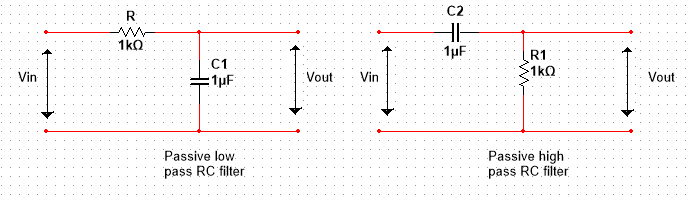
\includegraphics[width=0.70\textwidth]{graphics/passivehighlow.png}
    \caption{Passive low and high pass filters RC filter setups.}
    \label{fig:PassiveHighLow}
\end{figure}

Operational amplifiers or op amps are device that amplify voltage signals.
These devices are heavily used in signal conditioning and filtering.
The DC gains of op amps is a ratio between the input voltage and the output voltage. 

\begin{equation}
    A_v = \frac{V{out}}{V{in}} = 1 + \frac{R_f}{R_{in}}
    \label{eq:DCGain}
\end{equation}

The gain from a non inverting op amp can be found by \textit{Equation \ref{eq:DCGain}}, $A_v$ is the gain and $R_f$ and $R_{in}$ are the resistor values of the resistor configuration seen on the left hand side in \textit{Figure \ref{fig:invNonInvOPamp}}.


\begin{equation}
    A_v = -\frac{V{out}}{V{in}} = -\frac{R_f}{R_{in}}
    \label{eq:invertDCGain}
\end{equation}

The gain from a inverting op amp can be found by \textit{Equation \ref{eq:invertDCGain}}, $A_v$ is the gain and $R_f$ and $R_{in}$ are the resistor values of the resistor configuration seen on the right hand side in \textit{Figure \ref{fig:invNonInvOPamp}}.

\begin{figure}[h]
    \centering
    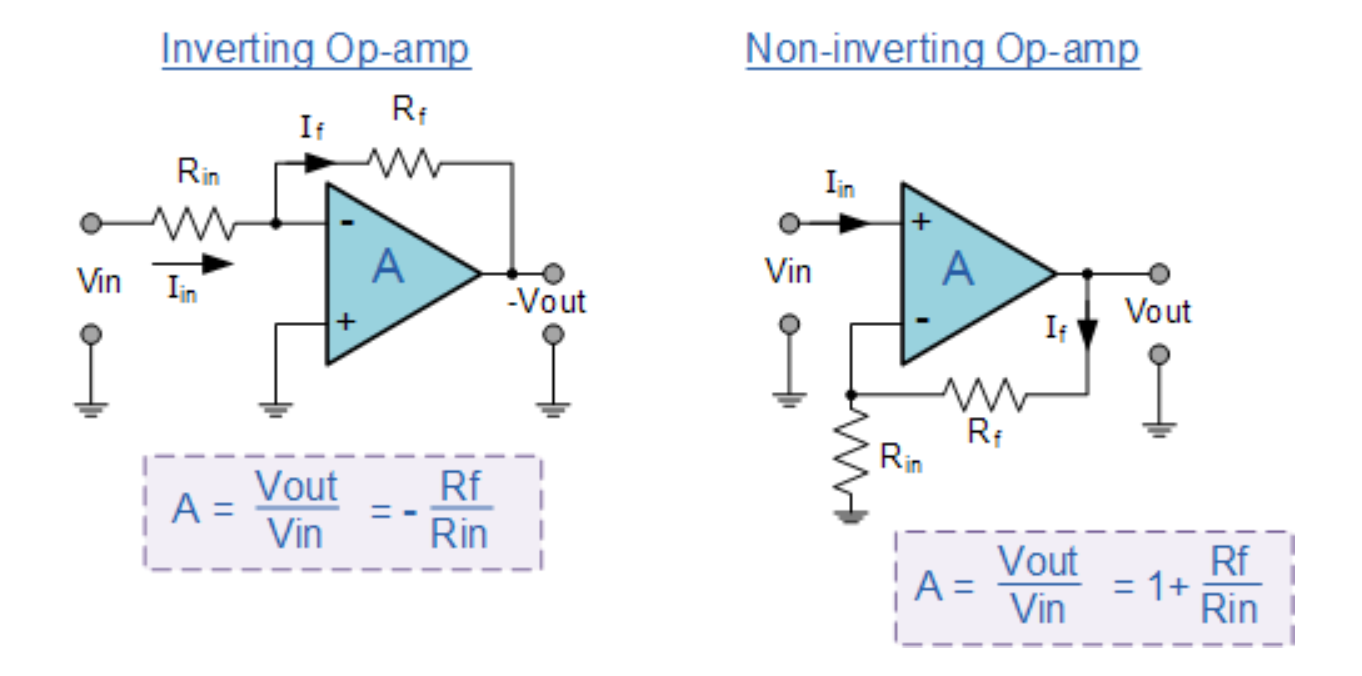
\includegraphics[width=0.70\textwidth]{graphics/invNoninv.png}
    \caption{Inverting and non inverting op amp setups \cite{noauthor_operational_2013}.}
    \label{fig:invNonInvOPamp}
\end{figure}

When the RC filter and op amps are combined, they form what is called an active filter.
Examples of which can be seen in \textit{Figures \ref{fig:LowPassFilter},\ref{fig:HighPassFiler}} and their respective frequency and phase shift responses in \textit{Figures \ref{fig:LowPassResponse},\ref{fig:HighPassResponse}}.
These filters performs the same as an RC filter in terms of its operations and frequency response with the addition of gain control \cite{noauthor_active_2013-1}.


\begin{equation}
    A_f = \frac{V{out}}{V{in}} = \frac{A_v}{\sqrt{1 + (\frac{f}{f_c})^2}}
    \label{eq:ActiveLowPass}
\end{equation}





The gain of the first order active low pass filter can be found using \textit{Equation \ref{eq:ActiveLowPass}}.
Where $A_f$ is the voltage gain, $A_v$ is the dc gain seen in \textit{Equation \ref{eq:DCGain}}, f is the frequency of the signal and $F_c$ is the set cutoff frequency.
This has the effect of active gain control depending on the frequency of the input.
When,
\begin{enumerate}
    \item $f < F_c$, $A_f \approx A_v$
    \item $f = F_c$, $A_f = \frac{A_v}{\sqrt{2}} = 0.707 A_v$
    \item$f > F_c$, $A_f < A_v$
\end{enumerate}

\begin{figure}[h]
    \centering
    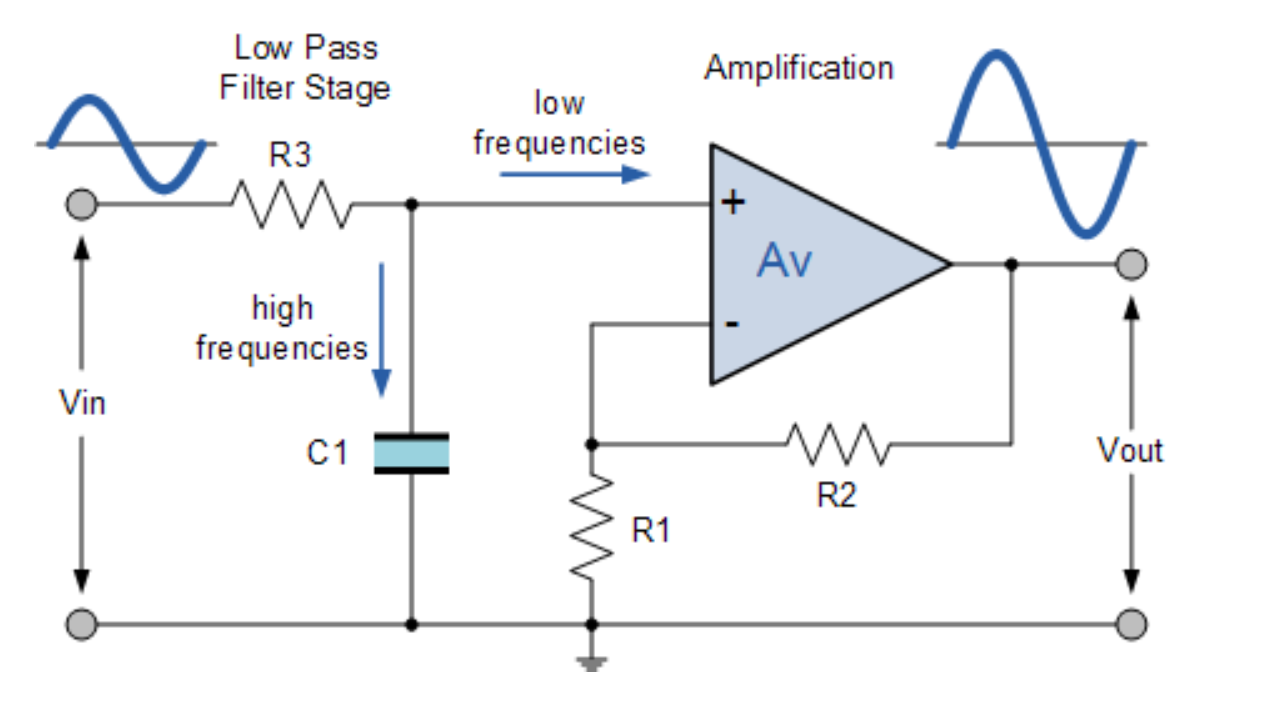
\includegraphics[width=0.70\textwidth]{graphics/lowPassFilter.png}
    \caption{Active first order low pass filter \cite{noauthor_active_2013-1}.}
    \label{fig:LowPassFilter}
\end{figure}

\begin{figure}[h]
    \centering
    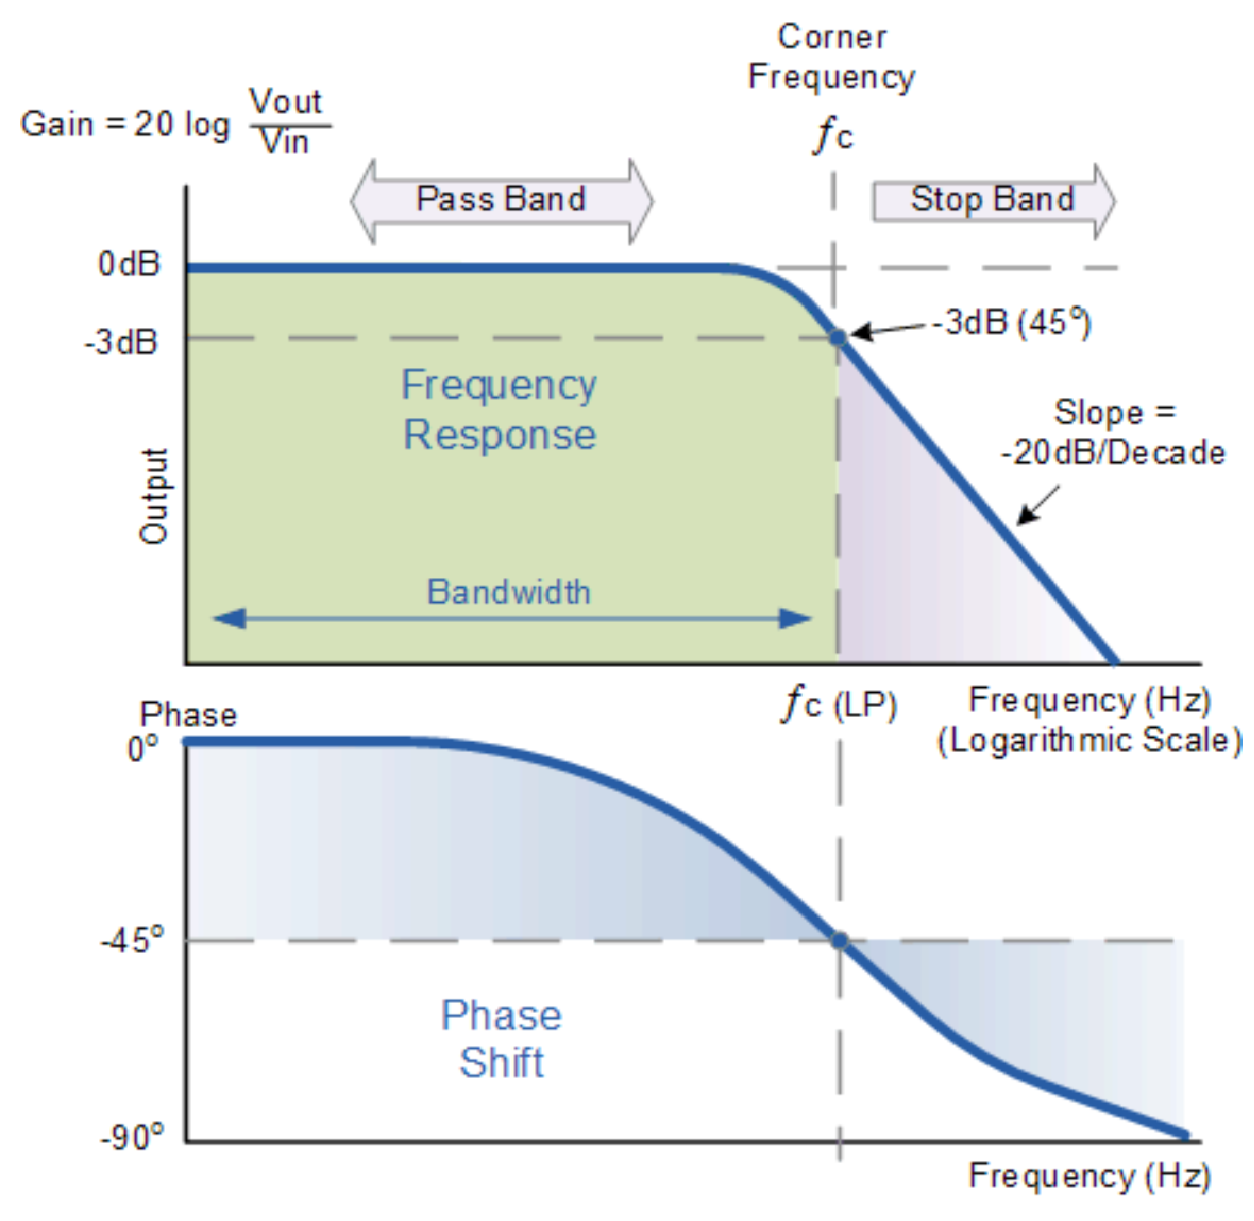
\includegraphics[width=0.70\textwidth]{graphics/lowPassResponse.png}
    \caption{First order RC low pass frequency response and phase shift \cite{noauthor_low_2013}}
    \label{fig:LowPassResponse}
\end{figure}

\begin{equation}
    A_f = \frac{V{out}}{V{in}} = \frac{A_v(\frac{f}{f_c})}{\sqrt{1 + (\frac{f}{f_c})^2}}
    \label{eq:ActiveHighPass}
\end{equation}

The gain of the first order active high pass filter can be found using \textit{Equation \ref{eq:ActiveHighPass}}.
Where $A_f$ is the voltage gain, $A_v$ is the dc gain seen in \textit{Equation \ref{eq:DCGain}}, f is the frequency of the signal and $F_c$ is the set cutoff frequency.
This has the effect of active gain control depending on the frequency of the input.
When,
\begin{enumerate}
    \item $f < F_c$, $A_f < A_v$
    \item $f = F_c$, $A_f = \frac{A_v}{\sqrt{2}} = 0.707 A_v$
    \item$f > F_c$, $A_f \approx A_v$
\end{enumerate}


\begin{figure}[h]
    \centering
    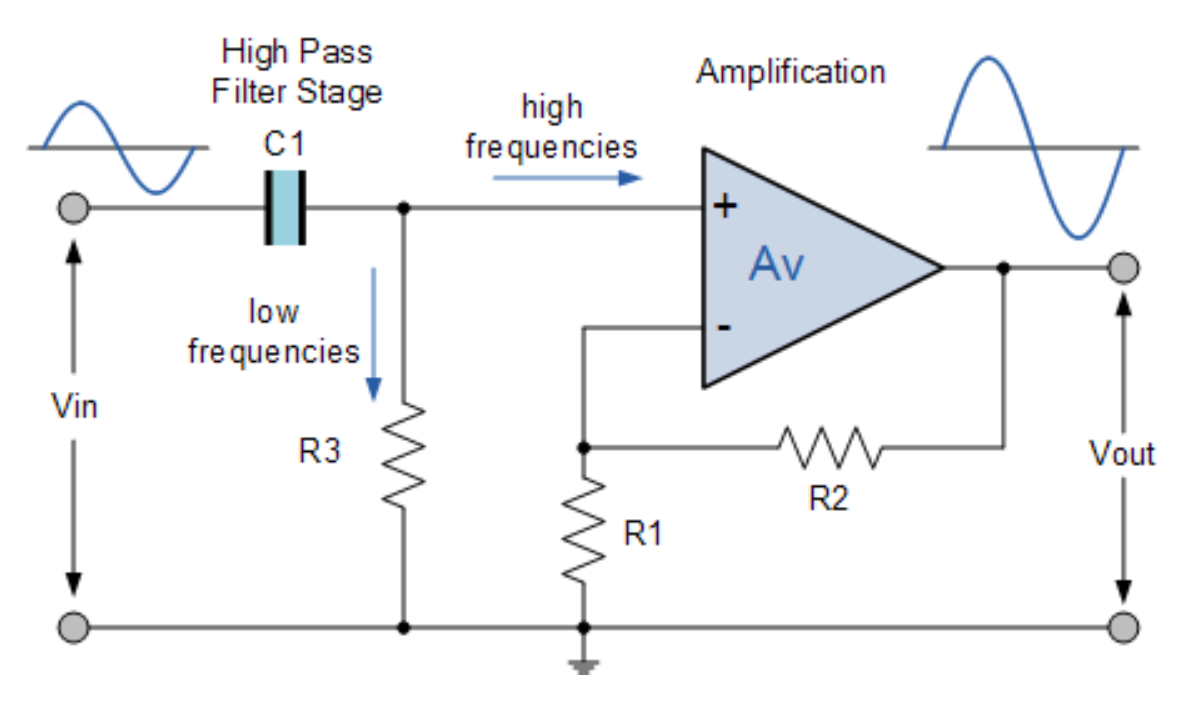
\includegraphics[width=0.60\textwidth]{graphics/highPassFilter.png}
    \caption{Active first order low pass filter \cite{noauthor_active_2013}.}
    \label{fig:HighPassFiler}
\end{figure}

\begin{figure}[h]
    \centering
    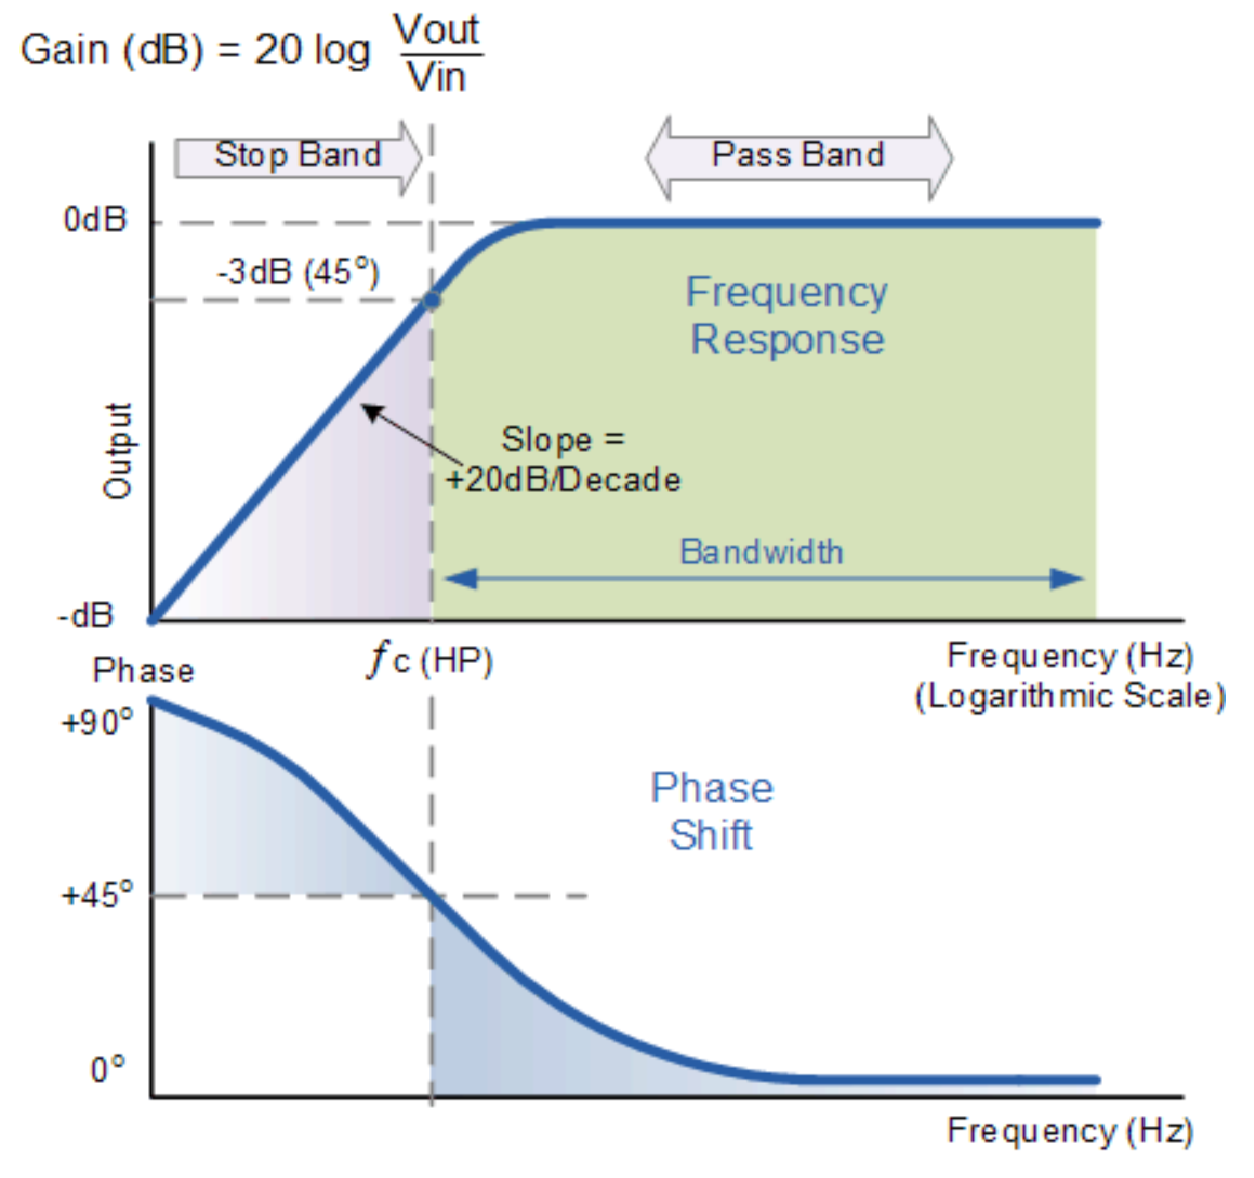
\includegraphics[width=0.60\textwidth]{graphics/highPassResponse.png}
    \caption{First order RC high pass frequency response and phase shift \cite{noauthor_high_2013}}
    \label{fig:HighPassResponse}
\end{figure}

\clearpage

Decibel is a relative unit of measure, used in electronic circuit to express ratio of input values to output value on a logarithmic scale.  

\begin{equation}
    dB = 20log\frac{V{out}}{V{in}}
    \label{eq:DBGAIN}
\end{equation}

The gain in decibel is found by \textit{Equation \ref{eq:DBGAIN}}, where $V{out}$ is the output root mean square (rms) voltage of the circuit and V{in} is the input rms voltage.

Summing amplifiers or summing inverter circuits are useful when combining two or more signals together.
An example of the circuit can be seen in \textit{Figure \ref{fig:SummingOpAmp}}, where $R_1 = R_2 = R_3$ would be the same value.
The circuit yields a voltage output that is equal to all the input voltages summed together, multiplied with the unity gain of the amplifier.
This is possible due to the virtual ground that is created by a non inverting op amp configuration\cite{noauthor_summing_2013}. 
This circuit is especially useful when there is a need to shift the signal from an oscillating AC voltage to an oscillating DC voltage.


\begin{figure}[h]
    \centering
    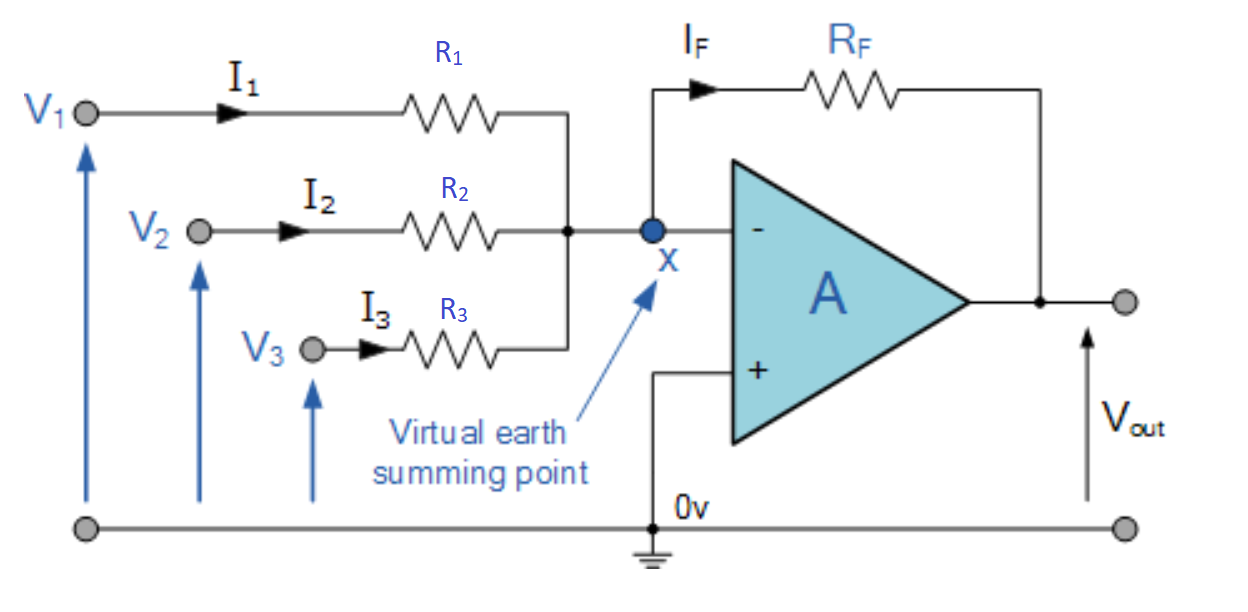
\includegraphics[width=0.70\textwidth]{graphics/SummingOpAmp.png}
    \caption{Scaling summing amplifier circuit \cite{noauthor_summing_2013}}
    \label{fig:SummingOpAmp}
\end{figure}


\begin{equation}
    I_F = I_1 + I_2 + I_3 = -[\frac{V_1}{R_{1}} + \frac{V_2}{R_{2}} + \frac{V_3}{R_{3}}]
\end{equation}


$$-V_{out} = \frac{R_F}{R_{1}}V_1 +\frac{R_F}{R_{2}}V_2 +\frac{R_F}{R_{3}}V_3$$

Scaling summing amplifiers are in the same configuration as summing amplifiers with one main difference which is that resistor values are not equal to one another.
This enables individual scaling of each signal, which means that each input signal can have different gain values.

\begin{equation}
    V_{out} = -R_F(\frac{V_1}{R_{1}} +\frac{V_2}{R_{2}} +\frac{V_3}{R_{3}} + ...)
    \label{eq:ScalingGain}
\end{equation}

Finding the output voltage can be found using \textit{Equation \ref{eq:ScalingGain}}.
Where $V_out$ is the output voltage, $R_f$ is the voltage across the input and output of the op amp, $R_1, R_2$ and $R_3$ are the resistor value of the different input signals.
Lets take for an example of an AC signal that needs to be shifted so that there is no negative voltage, see \textit{Figure \ref{fig:sumCircuitexamp}} for the layout of the circuit.
The AC signal (U1B\_out) would along with the shifting signal, in this case a DC voltage of 1.65V.
The AC signal is scaled by a factor of A = $\frac{180\Omega}{90\Omega}$ = 2.
How ever the DC voltage signal only scaled by a factor of A = $\frac{180\Omega}{180\Omega}$ = 1.
The voltage output, U1C\_out can be seen in \textit{Figure \ref{fig:SummingOpAmpShift}} as the red signal and the input signal, U1B\_out is represented by the white signal.
This creates a problem though, the output signal is shifted by $90\deg$ and the scaling op amp is in a inverting configuration the signal is inverted, so it is negative.
Both are fixed by the addition of U1D, an inverting amplifier.
Which puts the signal back in phase with the original input signal as well as it now is positive, as seen in \textit{Figure \ref{fig:SummingOpAmpShift1}} where the red signal is U1D\_out the output of the inverting amplifier and the white signal is the original input signal U1B\_out.


\begin{figure}[h]
    \centering
    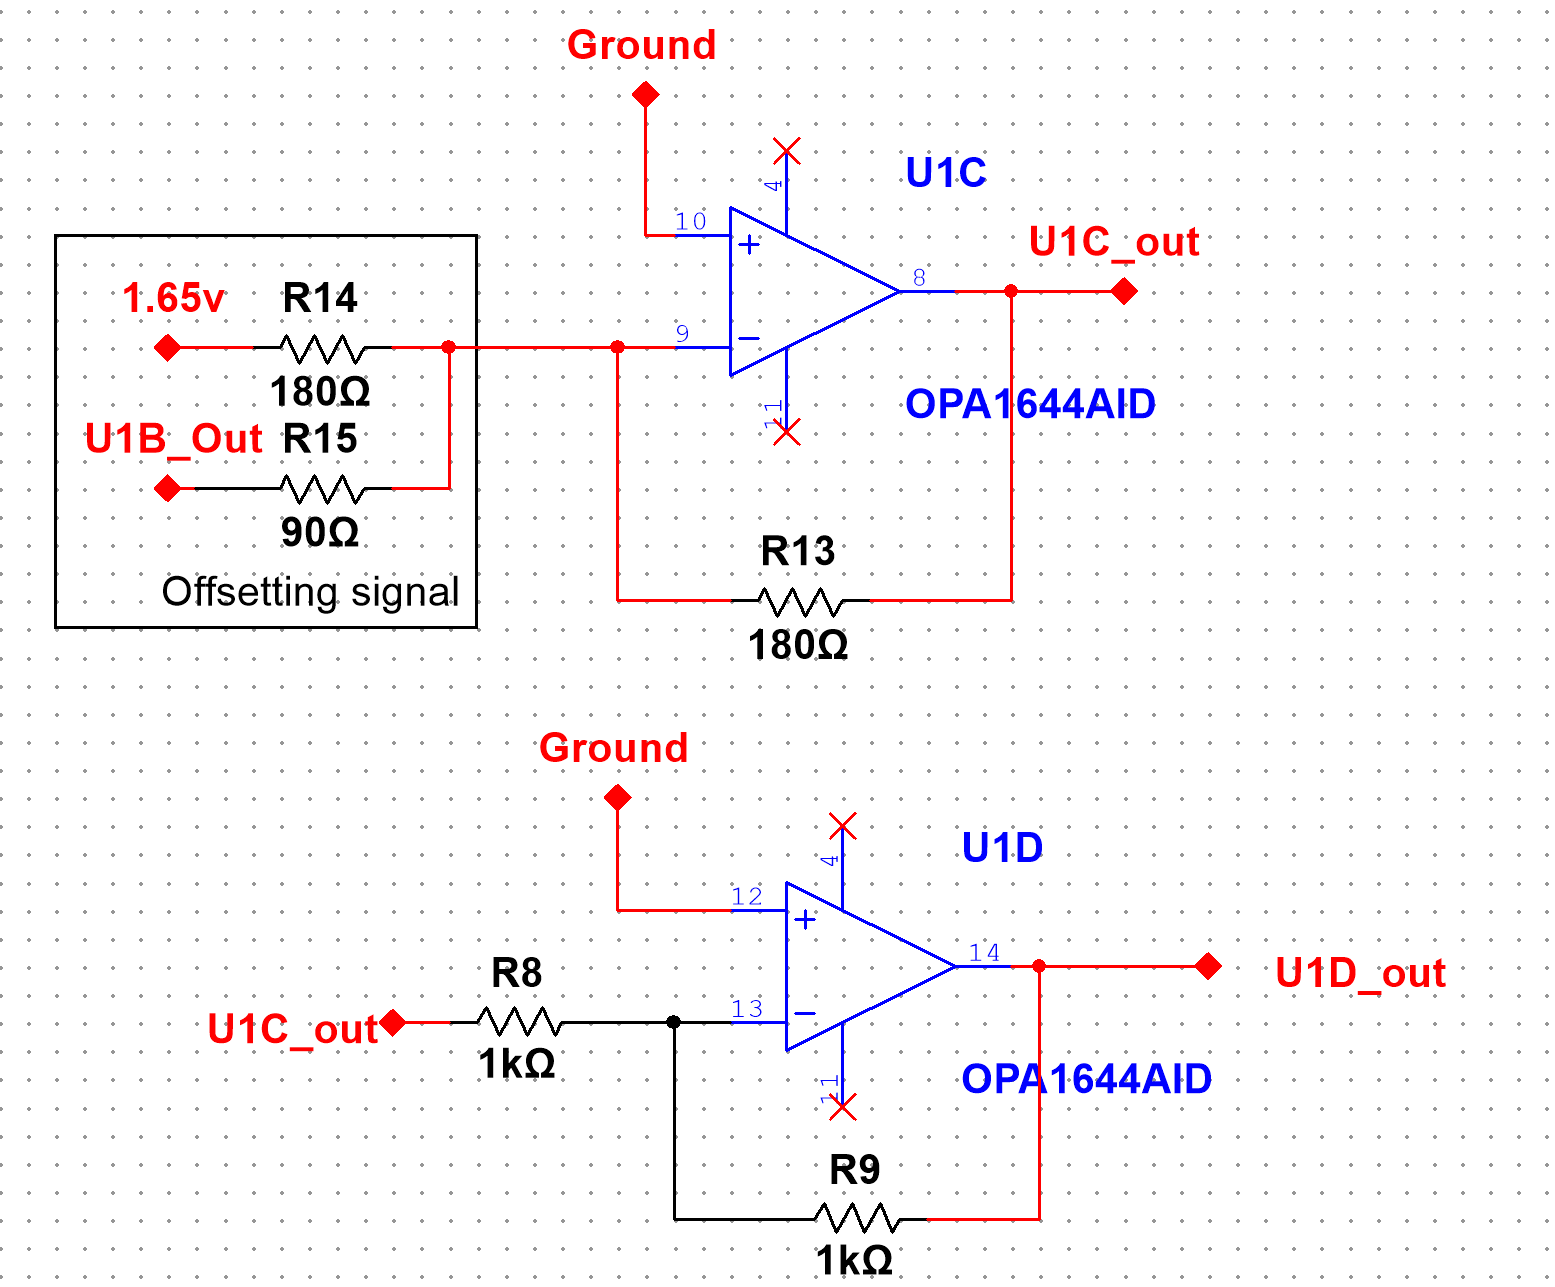
\includegraphics[width=0.70\textwidth]{graphics/sumCircuitexamp.png}
    \caption{Example of a scaling amplifier circuit where two signals are combined to create a shift of the original signal. U1C represents the scaling amplifier, U1D is a normal inverting amplifier.}
    \label{fig:sumCircuitexamp}
\end{figure}

\begin{figure}[h]
    \centering
    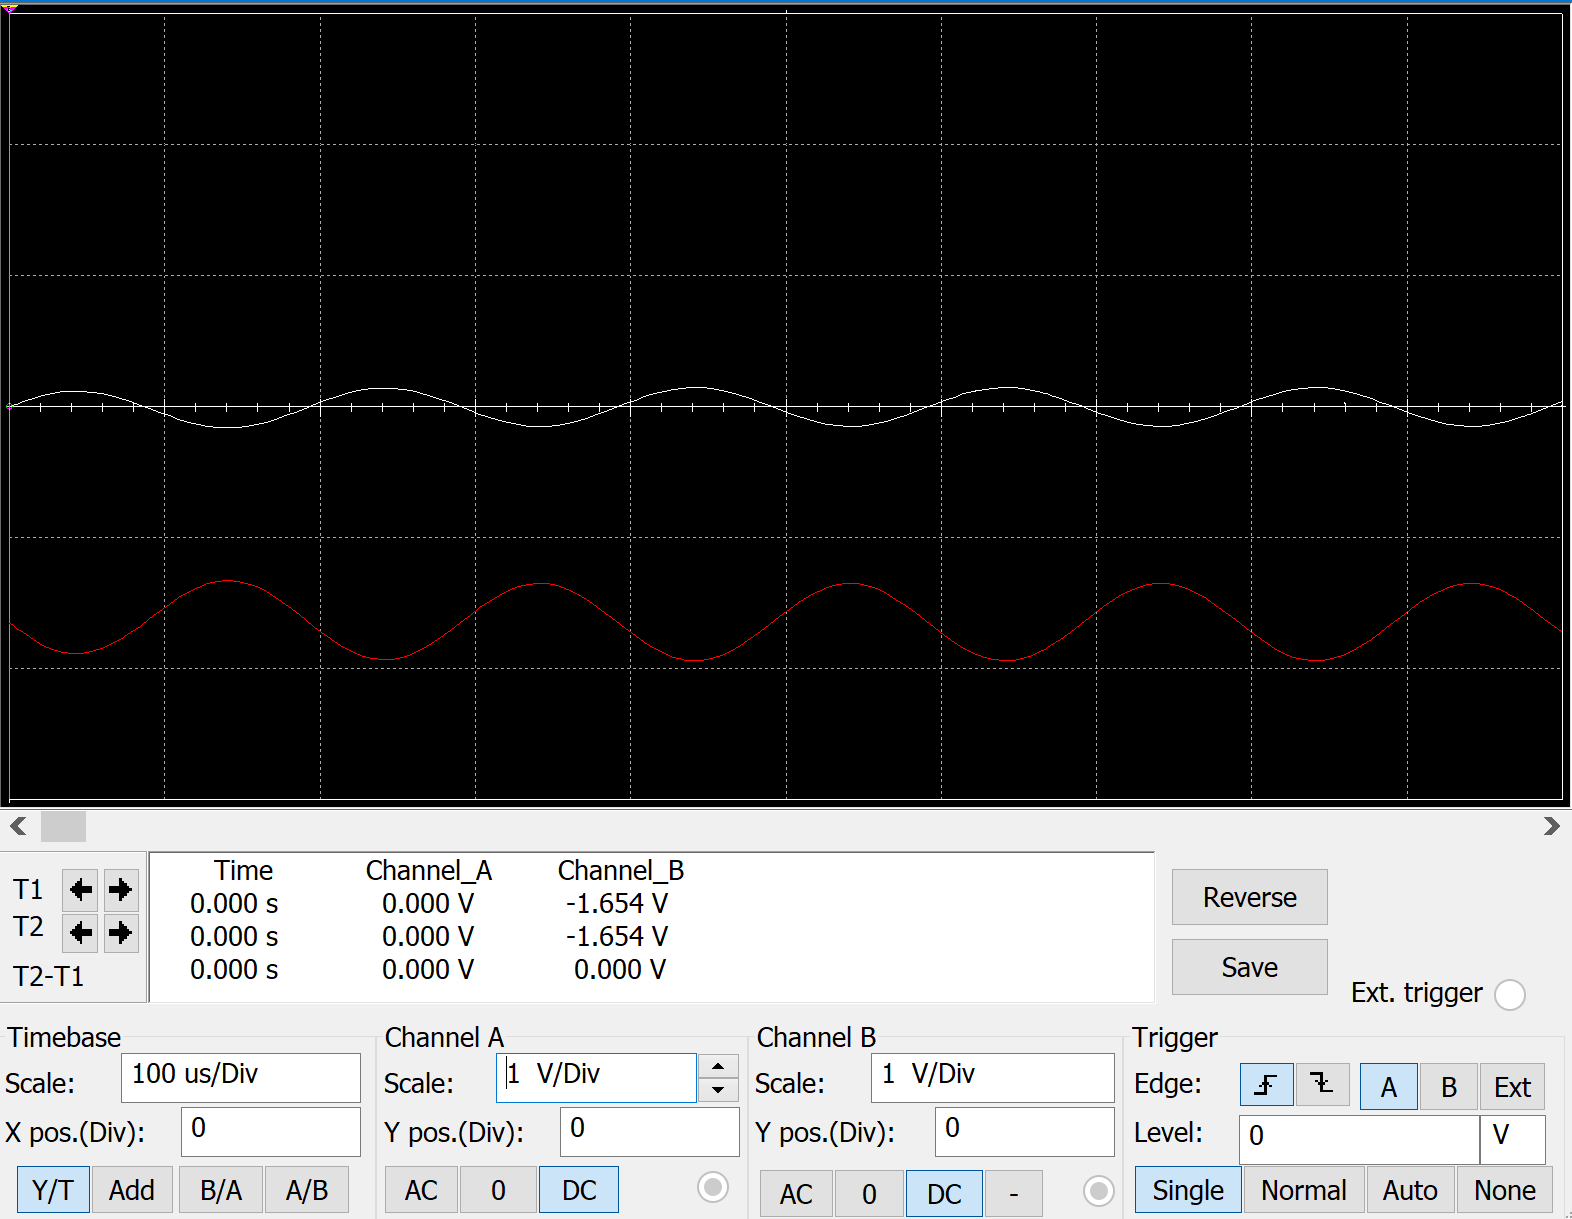
\includegraphics[width=0.70\textwidth]{graphics/summingShift.png}
    \caption{Example of the signal shift of a summing Op Amp circuit, the red signal represents the voltage output U1C\_out and the white signal is the input AC signal U1B\_out.}
    \label{fig:SummingOpAmpShift}
\end{figure}

\begin{figure}[h]
    \centering
    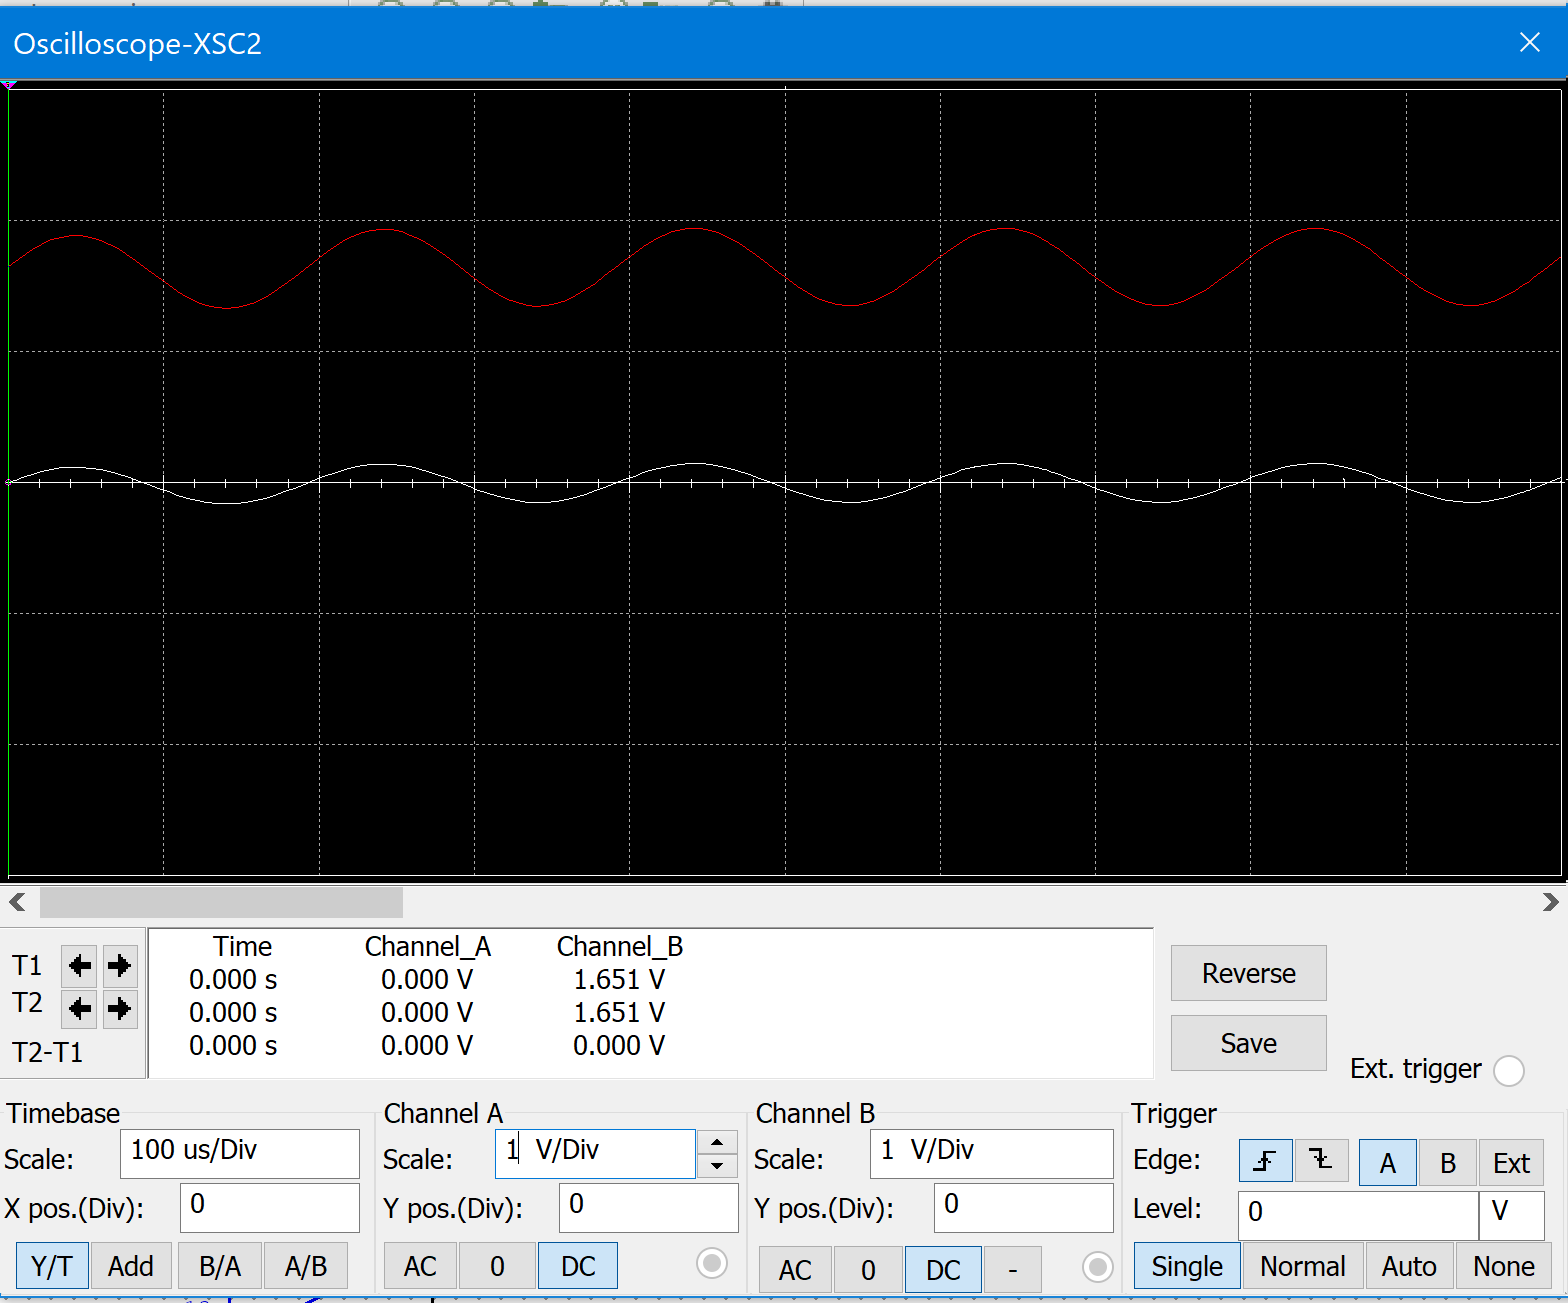
\includegraphics[width=0.70\textwidth]{graphics/summingShift1.png}
    \caption{Example of the signal shift of a summing Op Amp circuit, the red signal represents the voltage output U1D\_out and the white signal is the input AC signal U1B\_out}
    \label{fig:SummingOpAmpShift1}
\end{figure}


\clearpage

\fxfatal{SKOÐA H'ER-----------------------}
%ADC CHARECTERISTICS https://forum.pjrc.com/threads/44929-Teensy-3-5-ADC-characteristcs
%SD POSSIBLE https://forum.pjrc.com/threads/45993-Teensy-3-6-ADC-DMA-Question
%Teensy36ISRLogger Skilar með 8gb kortinu 6.67MB/s
%https://forum.pjrc.com/threads/49975-writing-binary-file-on-SD-card-in-Teency-3-5

\subsection{Microcontroller/Microcomputer}%Breyta um titil

For this project the most important factors when choosing a microcontroller/microcomputer were regarding the ADC specifications as well as the power consumption.\textbf{VITNA Í GOALS} tala um upplausn bit, power og fleira

\subsubsection{Arduino}

Arduino Uno is a programmable board that uses the 8-bit ATmega328p microcontroller.
Which is probably one of the most popular microcontroller in the world and the Arduino board is one of the among the best beginner boards to use because of the shear amount of documentation and tutorials for it.
The microcontroller main features can be seen in \textit{Table \ref{Tab:ATmega328p}}.


\begin{figure}[h]
    \centering
    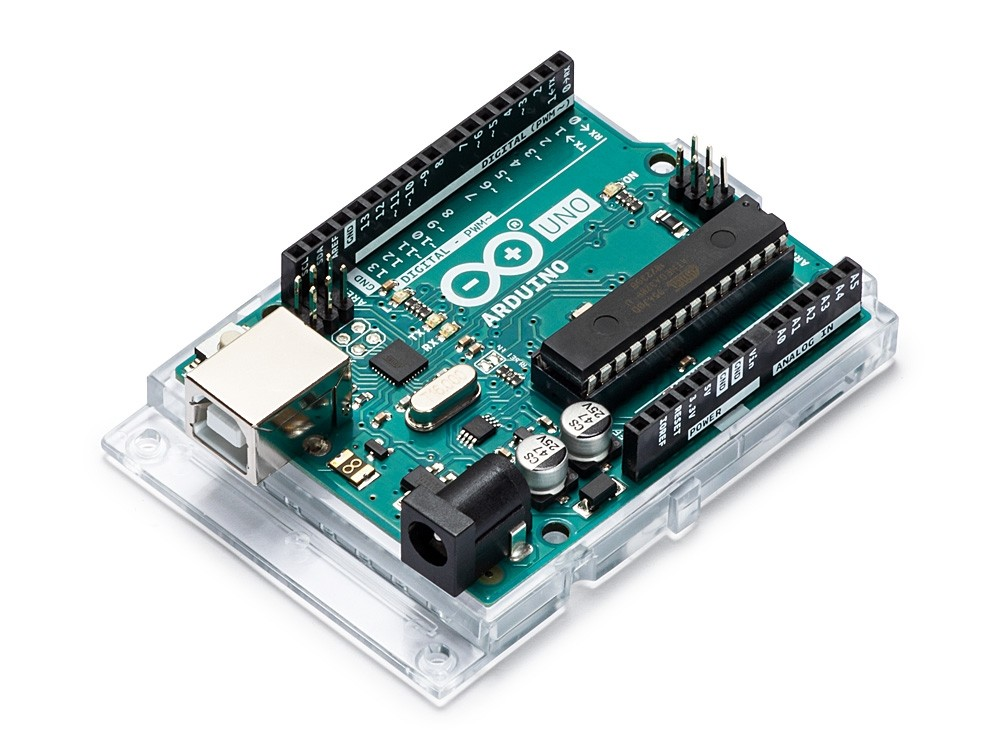
\includegraphics[width=0.70\textwidth]{graphics/ArduinoUNo.jpg}
    \caption{The Arduino Uno \cite{noauthor_arduino_nodate}}
    \label{fig:Arduino}
\end{figure}

\begin{table}[h]\caption{Main features of the ATmega328p \cite{noauthor_atmega328p_nodate}}.\label{Tab:ATmega328p}
\centering
    \begin{tabular}{|l|l|}
    \hline
        Parameters                        & Value                \\ \hline
        Flash memory [KB]                 & 32                      \\ \hline
        ADC resolution [bit]              & 10                   \\ \hline
        ADC sample speed [ksps]           & 15                     \\ \hline
        Digital Communication Peripherals & 1-UART, 2-SPI, 1-I2C \\ \hline
        Operating Voltage [V]             & 1.8 to 5.5           \\ \hline
        Max power consumption [W]         & 0.66               \\ \hline
        Price                             & 33\$                \\ \hline
    \end{tabular}
\end{table}


The Arduino has 14 digital input/output (I/O), and 6 can be used as pulse width modulation (PWM) outputs as well as 6 analog inputs.
The board has a USB connector which the board is programmed through as well as power it.
Arduino also provides its users with a free open source Arduino software integrated development environment (IDE).  \cite{noauthor_arduino_nodate}.
As well as a 6-channel 10-bit resolution ADC, with a conversion time of 65 to 260 $\mu s$ and up to 15 kilo samples per second (ksps) .
The board has a maximum current draw of 200mA, so at a operating voltage of 3.3V the power consumption is maximum 0.66W\cite{noauthor_atmega328p_nodate}.

%\textit{ It has 14 digital input/output pins (of which 6 can be used as PWM outputs), 6 analog inputs, a 16 MHz ceramic resonator (CSTCE16M0V53-R0), a USB connection, a power jack, an ICSP header and a reset button. It contains everything needed to support the microcontroller; simply connect it to a computer with a USB cable or power it with a AC-to-DC adapter or battery to get started.. You can tinker with your Uno without worrying too much about doing something wrong, worst case scenario you can replace the chip for a few dollars and start over again. "Uno" means one in Italian and was chosen to mark the release of Arduino Software (IDE) 1.0. The Uno board and version 1.0 of Arduino Software (IDE) were the reference versions of Arduino, now evolved to newer releases. The Uno board is the first in a series of USB Arduino boards, and the reference model for the Arduino platform; for an extensive list of current, past or outdated boards see the Arduino index of boards.}\cite{noauthor_arduino_nodate}.


\subsubsection{Raspberry Pi}

Unlike the Arduino the Raspberry Pi is not only a programmable microcontroller, but rather a single board microcomputer and is the third most sold computer brand worldwide \cite{noauthor_faqs_nodate}.
Currently there are 13 different model of the Raspberry Pi's with varying pricing and capabilities  some of which can be seen in \textit{Table \ref{Tab:RaspbModel}}. 
Raspberry Pis can be used with several operating system, for instance Linux, FreeBSD or a Raspberry pi OS that can come with or without a desktop.

\begin{center}
\begin{table}[h]\caption{Comparison of different Raspberry Pi models\cite{noauthor_faqs_nodate}}.\label{Tab:RaspbModel}
    \begin{tabular}{|l|l|l|l|c|}
    \hline
    \textbf{\begin{tabular}[c]{@{}l@{}}Raspberry Pi\\ Product\end{tabular}}        & \textbf{SoC} & \textbf{Speed} &  \textbf{\begin{tabular}[c]{@{}l@{}}Recommended\\ power supply \\ current capacity\end{tabular}} & \textbf{\begin{tabular}[c]{@{}l@{}}Typical bare-\\board current \\ consumption\end{tabular}} \\ \hline
     Model A+   & BCM2835      & 700MHz         & 0.7A          & 0.2A            \\ \hline
     Model B+   & BCM2835      & 700MHz         & 1.8A          & 0.33A            \\ \hline
     2 Model B  & BCM2836/7    & 900MHz         & 1.8A          & 0.5A                 \\ \hline
     3 Model B  & BCM2837A0/B0 & 1200MHz        & 2.5A          & 0.4A                  \\ \hline
     3 Model A+ & BCM2837B0    & 1400MHz        & 2.5A          & 0.35A                  \\ \hline
     3 Model B+ & BCM2837B0    & 1400MHz        & 2.5A          & 0.5A                  \\ \hline
     4 Model B  & BCM2711      & 1500MHz        & 3.0A          & 0.6A                  \\ \hline
     Zero       & BCM2835      & 1000MHz        & 1.2A          & 0.1A                   \\ \hline
     Zero W     & BCM2835      & 1000MHz        & 1.2A          & 0.15                  \\ \hline
     Zero WH    & BCM2835      & 1000MHz        & 1.2A          & 0.15                  \\ \hline
     400        & BCM2711      & 1800MHz        & 3.0A          & 0.8A                  \\ \hline
    \end{tabular}
\end{table}
\end{center}

Raspberry recommends powering the Raspberry Pi using 5V.
This means that the Raspberry Pi uses quite a bit of power,Raspberry Pi Zero (6W) Raspberry Pi 2 B (9W), Raspberry Pi 3(12.5W).
Taking a closer look at the Raspberry Pi Zero since it fits within the power consumption specifications.
The microcomputer costs around 30 \$, has a 1GHz single-core CPU, 512MB RAM, Mini HDMI port, Micro USB OTG port,
Micro USB power and HAT-compatible 40-pin header.
It has i2c, SPI, PWM and serial pins, all GPIO pins are digital and can be configured to be input or output pins.
which can be seen in \textit{Figure \ref{fig:RPIGPIO}}.

\begin{figure}[h]
    \centering
    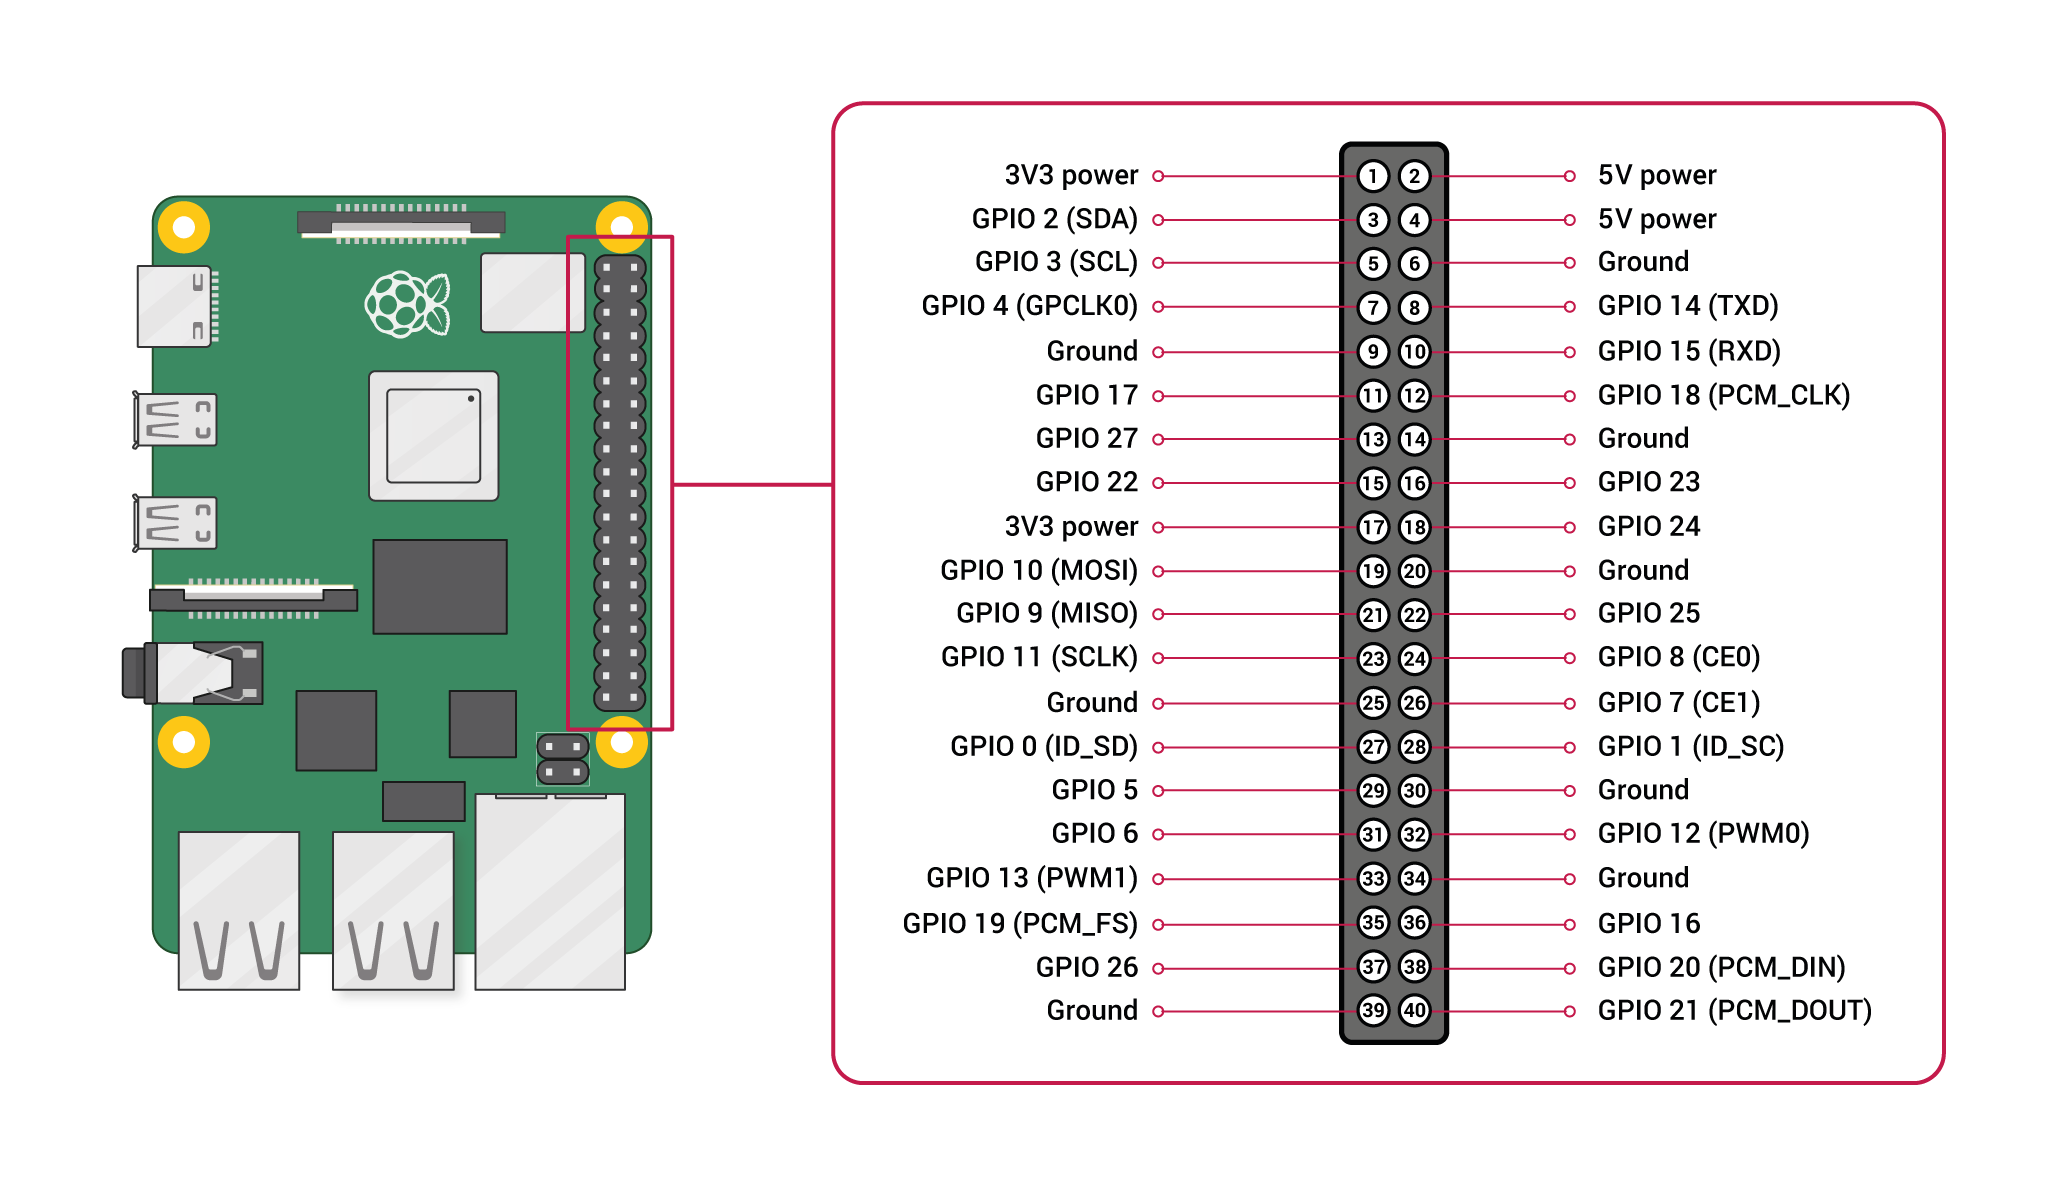
\includegraphics[width=0.70\textwidth]{graphics/ZeroGPIO.png}
    \caption{GPIO of the Raspberry Pi Zero \cite{noauthor_gpio_nodate}}
    \label{fig:RPIGPIO}
\end{figure}

The Raspberry Pi is however limited in the fact that it has no analog I/O pins, meaning that it can not convert analog to digital signal on its own.
However there is a way to record audio, which is done through sound card.
Several solutions have already been made available for this such as the Audio Injector stereo sound card which can directly connect to the general purpose input output (GPIO) pins of Raspberry Pi2, Pi3 and Pi Zero.
The card is made for an electret microphone and can supply the Raspberries with input and output audio.
The card has stereo RCA input and output, a headphone jack and a preamplifier, a volume knob and a low latency of 540 $\mu$s for both the input and output \cite{noauthor_rpi_nodate}.

\begin{figure}[h]
    \centering
    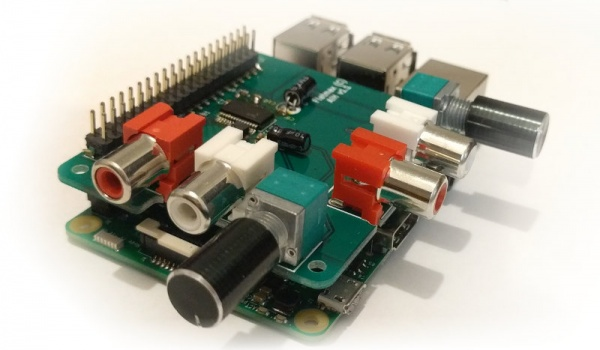
\includegraphics[width=0.70\textwidth]{graphics/rpisoundcard.jpg}
    \caption{The Audio Injector stereo sound card \cite{noauthor_rpi_nodate}}
    \label{fig:rpisoundcard}
\end{figure}


\subsubsection{Teensy}

Teensy's are the same as Arduino as being a USB programmable single board microcontroller.
The boards are can be programmed with multiple of programs such as the Arduino IDE software and can use both the examples and libraries that come with the program.
This is possible through an addition called Teensyduino which allso includes a large library for programing.
Other programs include Visual Micro, which enables programming on Visual Studio Code, PlaformIO IDE and CircuitPython (only available on Teensy 4.X) which allows python programming.
There are multiple models available, ranging in price, size and capabilities as seen in \textit{Table \ref{Tab:TeensyModel}}.


\begin{table}[h]\caption{Comparison of different Teensy models\cite{noauthor_teensy_nodate}}.\label{Tab:TeensyModel}
\begin{tabular}{|l|l|l|l|l|}
\hline
\multicolumn{1}{|c|}{\textbf{Specification}} & \multicolumn{1}{c|}{\textbf{Teensy 2.0}}                               & \multicolumn{1}{c|}{\textbf{Teensy 3.0}}                                            & \multicolumn{1}{c|}{\textbf{Teensy 3.5}}                                                  & \multicolumn{1}{c|}{\textbf{Teensy 4.1}}                                              \\ \hline
Processor & \begin{tabular}[c]{@{}l@{}}ATMEGA32U4\\ 8 bit AVR\\ 16 MHz\end{tabular} & \begin{tabular}[c]{@{}l@{}}MK20DX128\\ 32 bit ARM\\ Cortex-M4\\ 48 MHz\end{tabular} & \begin{tabular}[c]{@{}l@{}}MK64FX51\\2VMD12\\ 32-bit ARM\\ Cortex- M4\\ 120MHz\end{tabular} & \begin{tabular}[c]{@{}l@{}}MIMXRT1062\\ 32 bit ARM\\ Cortex-M7\\ 600 MHz\end{tabular} \\ \hline
\begin{tabular}[c]{@{}l@{}}Flash Memory\\ {[KB]}\end{tabular} & 32 & 131 & 512 & 7936 \\ \hline
%\begin{tabular}[c]{@{}l@{}}RAM Memory\\ (Bytes)\end{tabular}& 2560 & 16384 & 256K & 1024K \\ \hline
%\begin{tabular}[c]{@{}l@{}}EEPROM\\ (Bytes)\end{tabular} & 1024 & 2048 & 4096 & 4096 \\ \hline
\begin{tabular}[c]{@{}l@{}}Direct Memory\\ Access [Channels]\end{tabular}  & - & 16 & 16 & 32 \\ \hline
%I/O [Pins, V] & 25, 5 Volt & 34, 3.3 V & \begin{tabular}[c]{@{}l@{}}64, 3.3V,\\ 5V tol\end{tabular} &\begin{tabular}[c]{@{}l@{}}55, 3.3V,\\ 5V tol\end{tabular}   \\ \hline
\begin{tabular}[c]{@{}l@{}}ADC resolution\\ {[bit]}\end{tabular} & 10 & 16 & 16   & 12     \\ \hline
%PWM & 7 & 10 & 20 & 35 \\ \hline
UART,I2C,SPI & 1,1,1 & 3,1,1 & 6,3,3 & 8,3,3 \\ \hline
Price [\$] & {16.00} & {19.00} & {24.25} & {26.85} \\ \hline
\end{tabular}
\end{table}

Taking a closer look at the comparison between the Teensy 3.5 and Teensy 4.1.
Teensy 3.5 has 2 16bit, 416 ksps (in 16 bit mode) and 818.3 ksps for (<= 13 bit mode), 12MHz ADC\cite{freescale_semiconductor_kinetis_2021-1} and has a voltage range of 0-3.3V as well as some are 5V tolerant while the Teensy 4.1 offers 12 bits of resolution and 20MHz (samples per second is not specified) a range of 0 - 3.3V.
%The Teensy 3.5 also has an option of using pins connected to differential amplifiers, which can decrease unwanted noise of input analog signals.
%Teensy 3.5 also has two Digital to analog converters (DACs) output.
%Which makes it capable of outputting audio signals.
Both Teensys have a voltage regulator which reduces the 5V VUSB / VIN power to 3.3V for use by the main processor and most other parts. Additional circuitry may be powered from the 3.3V pin.
The recommended maximum for external 3.3V usage is 250mA or 0.825W.
When Teensy 3.5 is running at 120MHz processor speed it consumes roughly 50mA or 0.165W.
While the Teensy 4.0 consumes roughly 100mA or 0.33W at 600MHz processor speed.
%When power is not applied to VUSB or VIN, it is however possible to run by externally applying 3.3V power.
%There are two ways to power the Teensy's, the first one is to power them via USB.
%The Teensys are equipped with a voltage regulator which regulates the USB voltage of 5V down to 3.3V.
%They can also be powered straight to a VIN pin, which is recommended as a maximum of 3.3V and a 250mA %draw.
\cite{noauthor_teensy_nodate-1}%4.1
\cite{noauthor_teensy_nodate-2}.%3.5


\subsection{FINNA TITIL}

\subsubsection{Direct memory access}

When transferring data between main memories and I/O devices, direct memory access (DMA) can be utilized.
The benefit of using DMA for the data transfer is that it minimizes or eliminates the processors involvement with the data transfer.
The processor only initializes the DMA controller by configuring the read and write memory, size of data for each transfer and I/O address.
In \textit{Figure~\ref{fig:DMAcontroller}} the process of the data transfer is better explained.

\begin{figure}[h]
    \centering
    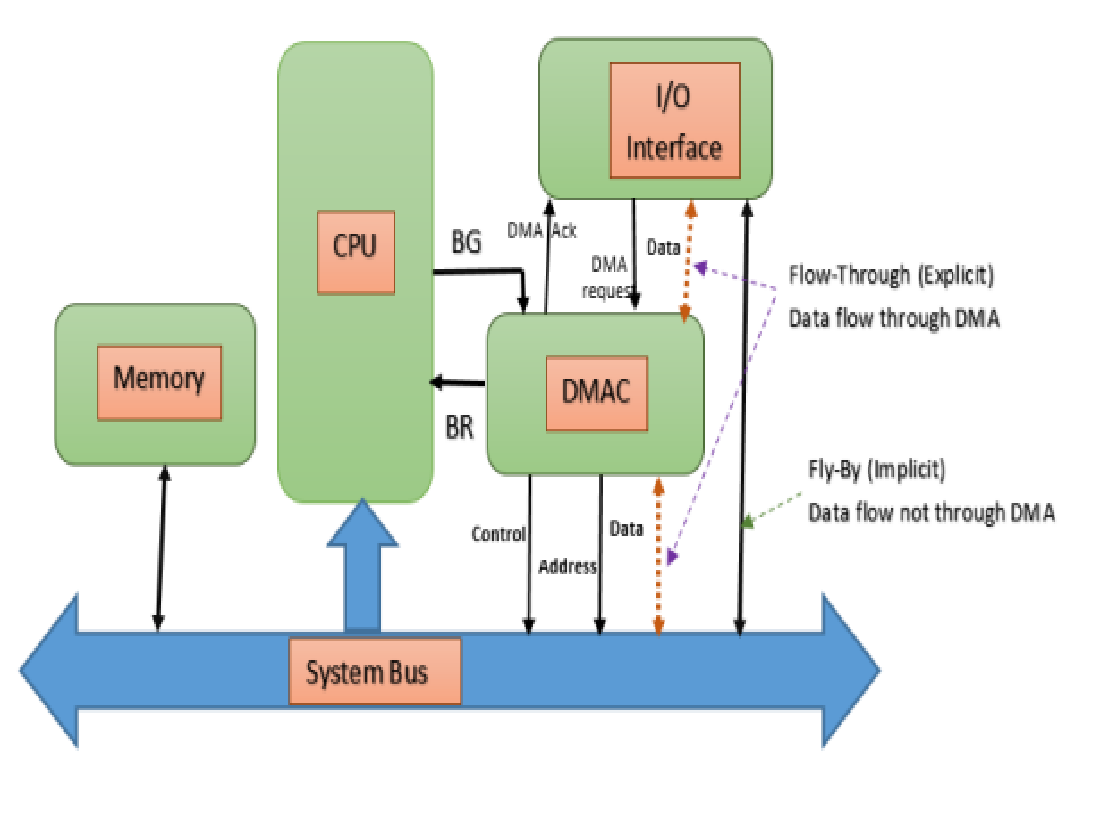
\includegraphics[width=0.70\textwidth]{graphics/DMA.png}
    \caption{Data transfer for a DMA controller. Where the data transfers from the I/O device directly to memory. \cite{ahmed_design_2019}}
    \label{fig:DMAcontroller}
\end{figure}

Bus request (BR) signal is sent to the processor during the data transfer operation.
The processor then finishes its current job and replies with a bus grant (BG) signal.
The DMA controller receives the signal and can then initiate the data transfer.
There are two modes in which the DMA can perform data transfers.
The first is called flow through, where the data flows through the DMA controller between the I/O device to memory.
The second is called fly by, where the data is transferred directly between the I/O device and memory \cite{ahmed_design_2019}.


%%% Local Variables: 
%%% mode: latex
%%% TeX-master: "DEGREE-NAME-YEAR"
%%% End: 
%%RUM: "Methods"
\part{The Second Part}
\chapter{Results}

%In this section you discuss any issues that came up while developing the system.  If you found something particularly interesting, difficult, or an important learning experience, put it here.  This is also a good place to put additional figures and data.


\section{Code}


All codes were developed in Arduino IDE using a teensyduino extension.
Since this project is about the data acquisition of cetacean vocalization, all codes were developed to read analog signals and write the value to a file on a SD card.
The SD card used was a Samsung EVO Plus microSDHC 32 GB, capable of 95MB/s read speed and 20MB/s write speed.
This should be sufficient since the data is 2 bytes per sample which means in theory the card should be able to handle a peak of 10Msps.



%\textbf{SKOÐAFYRIR UTERIKNGA Á CONVERSION T'IMA!!!!!!!!!!!!!!!!}
% https://www.pjrc.com/teensy/K64P144M120SF5RM.pdf bls 859

\subsection{ContinousAnalogRead}

The basic function of the code is simple, it should read a 64KB buffer of analog values from the circuit as well as save the microseconds of each read in a different buffer.
Once the buffers are full, the program begins to write all the buffers to the SD card.
To configure the ADC, the ADC library by pedvide was used \cite{villanueva_pedvideadc_2021}.
The library handles the configuration of the built-in ADC and should make that process easier, however it makes it a little harder to see what exactly configures the ADC to be.
To use the library, the code must first create an ADC object via 
$ADC *ADC = new ADC();$
which is then used to define the attributes of the ADC, which can be seen in %lines 69 - 83 in~
\textit{Listing~\ref{src:ContAnalogRead}}. 
The reference voltage is set as 3.3V, to have a voltage range of 0 - 3.3V.
The ADC averaging is set to 0, which after testing was the fastest configuration.
The conversion speed of the ADC was set to the fastest setting for 16bits conversion or HIGH\_SPEED\_16BITS, which sets the ADC clock to $<= 12 MHz$.
Then the sampling speed was set to the fastest setting of VERY\_HIGH\_SPEED, which adds +0 cycles to the ADC clock (ADCK).
The library can as well be configured so that once a conversion occurs an ISR is triggered which is done by enabling an interrupts function and ties the conversion of adc0 to void adc0\_isr.
To set the ADC to do a continuous conversion, startContinuous() is used and can be configured to a specific pin on the Teensy.
Finally the results of the conversion are found using analogReadContinuous().

Once the ADC is configured, the device can start reading analog values.
It collects the analog readings to a buffer as well as the timestamp of each reading.
Once the buffers are full, the program writes to a SD card.
It writes both values as decimal values to a text file on the card.
The analog read and writes to SD card can be seen in \textit{Figure~\ref{fig:ContAnalSpeed}}

\begin{figure}[h]
    \centering
    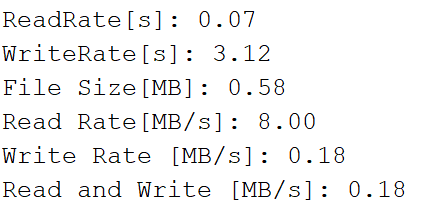
\includegraphics[width=0.50\textwidth]{graphics/ContinousReadSpeed.png}
    \caption{The read and write speeds of ContinuousAnalogRead.ino}
    \label{fig:ContAnalSpeed}
\end{figure}


The data recorded by the device with the ContinuousAnalogRead.ino as the code. 
With an input signal of 10$mV_{pp}$ and 50kHz frequency. 
It appears to run too fast for the ADC, seeing as it has several conversions made at each voltage level as seen in \textit{Figure~\ref{fig:ContAnalREsults}}, every three data point a new conversion occurs.
Even though it should wait until the ADC is ready for a new conversion it does not appear to do so.


\begin{figure}[h]
    \centering
    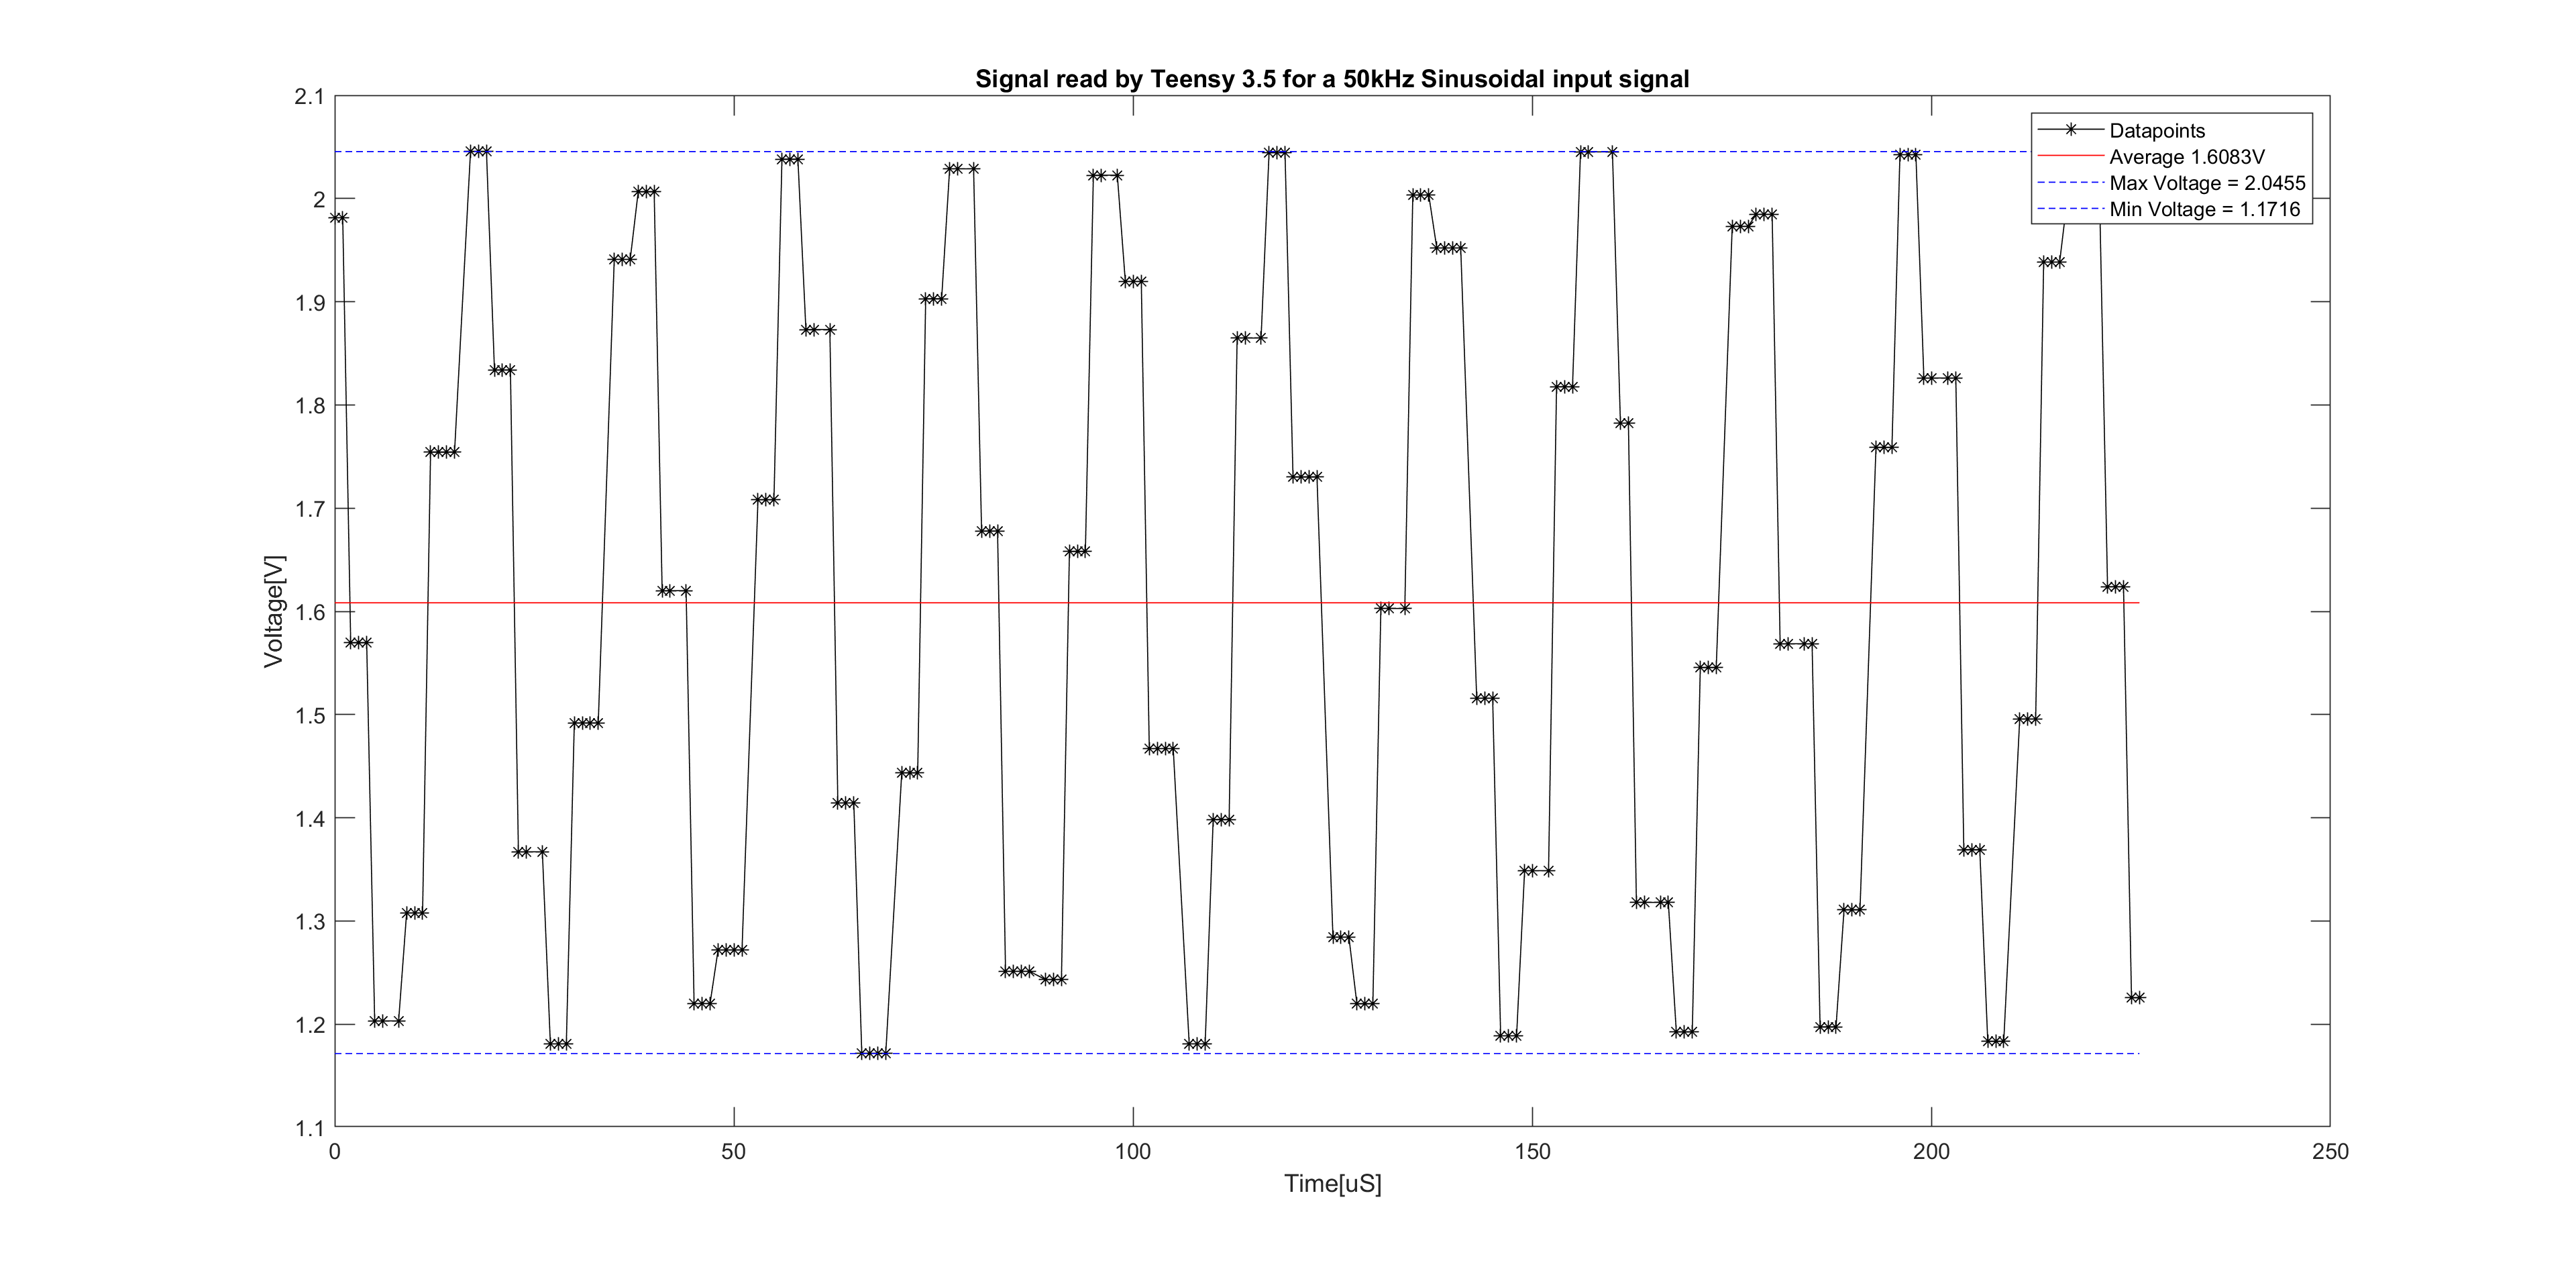
\includegraphics[width=1.0\textwidth]{graphics/COntANalogResults.png}
    \caption{Results from Teensy using ContinuousAnalogRead.ino.}
    \label{fig:ContAnalREsults}
\end{figure}

Just before the test, a single reading of the output signal was taken with an oscilloscope which can be seen in \textit{Figure~\ref{fig:ContAnalOscillascope}}.

\begin{figure}[h]
    \centering
    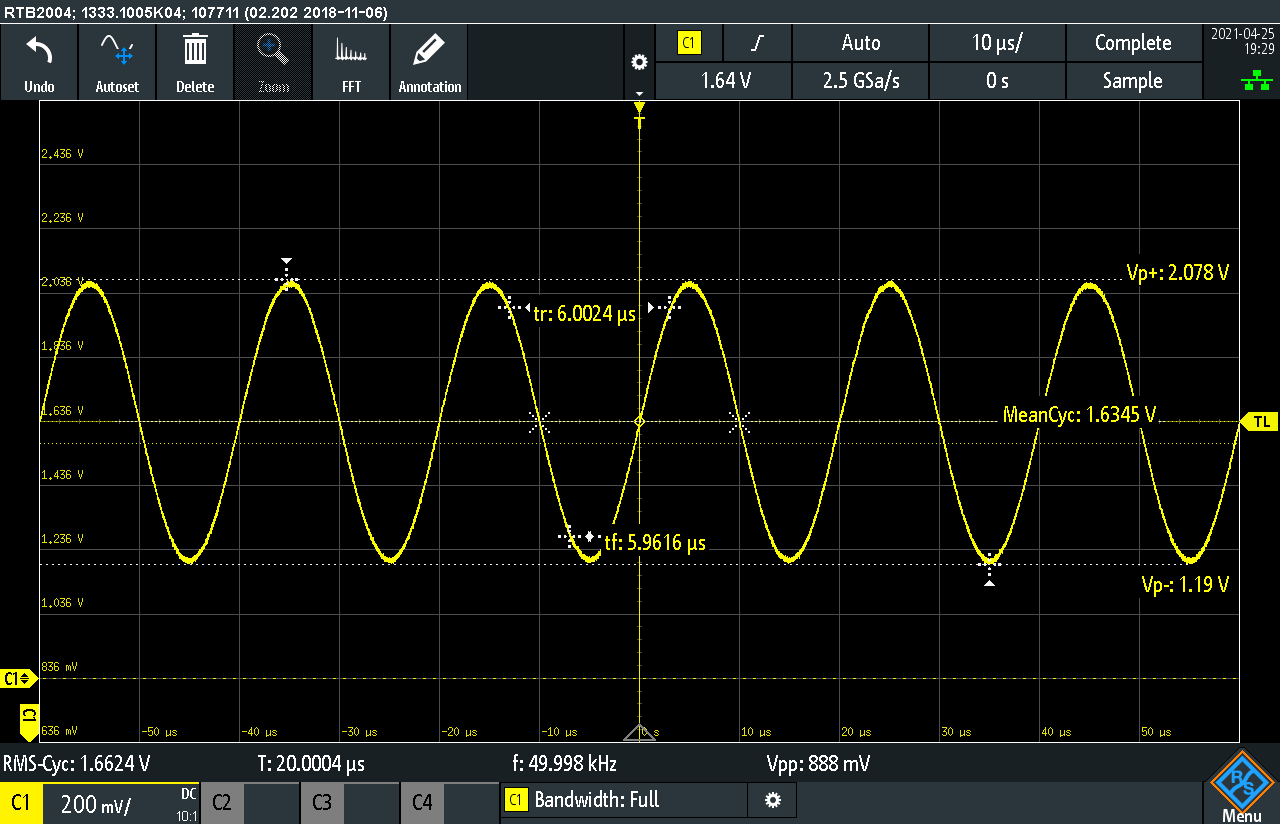
\includegraphics[width=0.70\textwidth]{graphics/ContAnalogReadOscillascope.PNG}
    \caption{Oscilloscope readings of the output signal}
    \label{fig:ContAnalOscillascope}
\end{figure}

\vspace{4cm}
%\begin{figure}[h]
%    \subfloat[\textbf{Sub figure caption}]{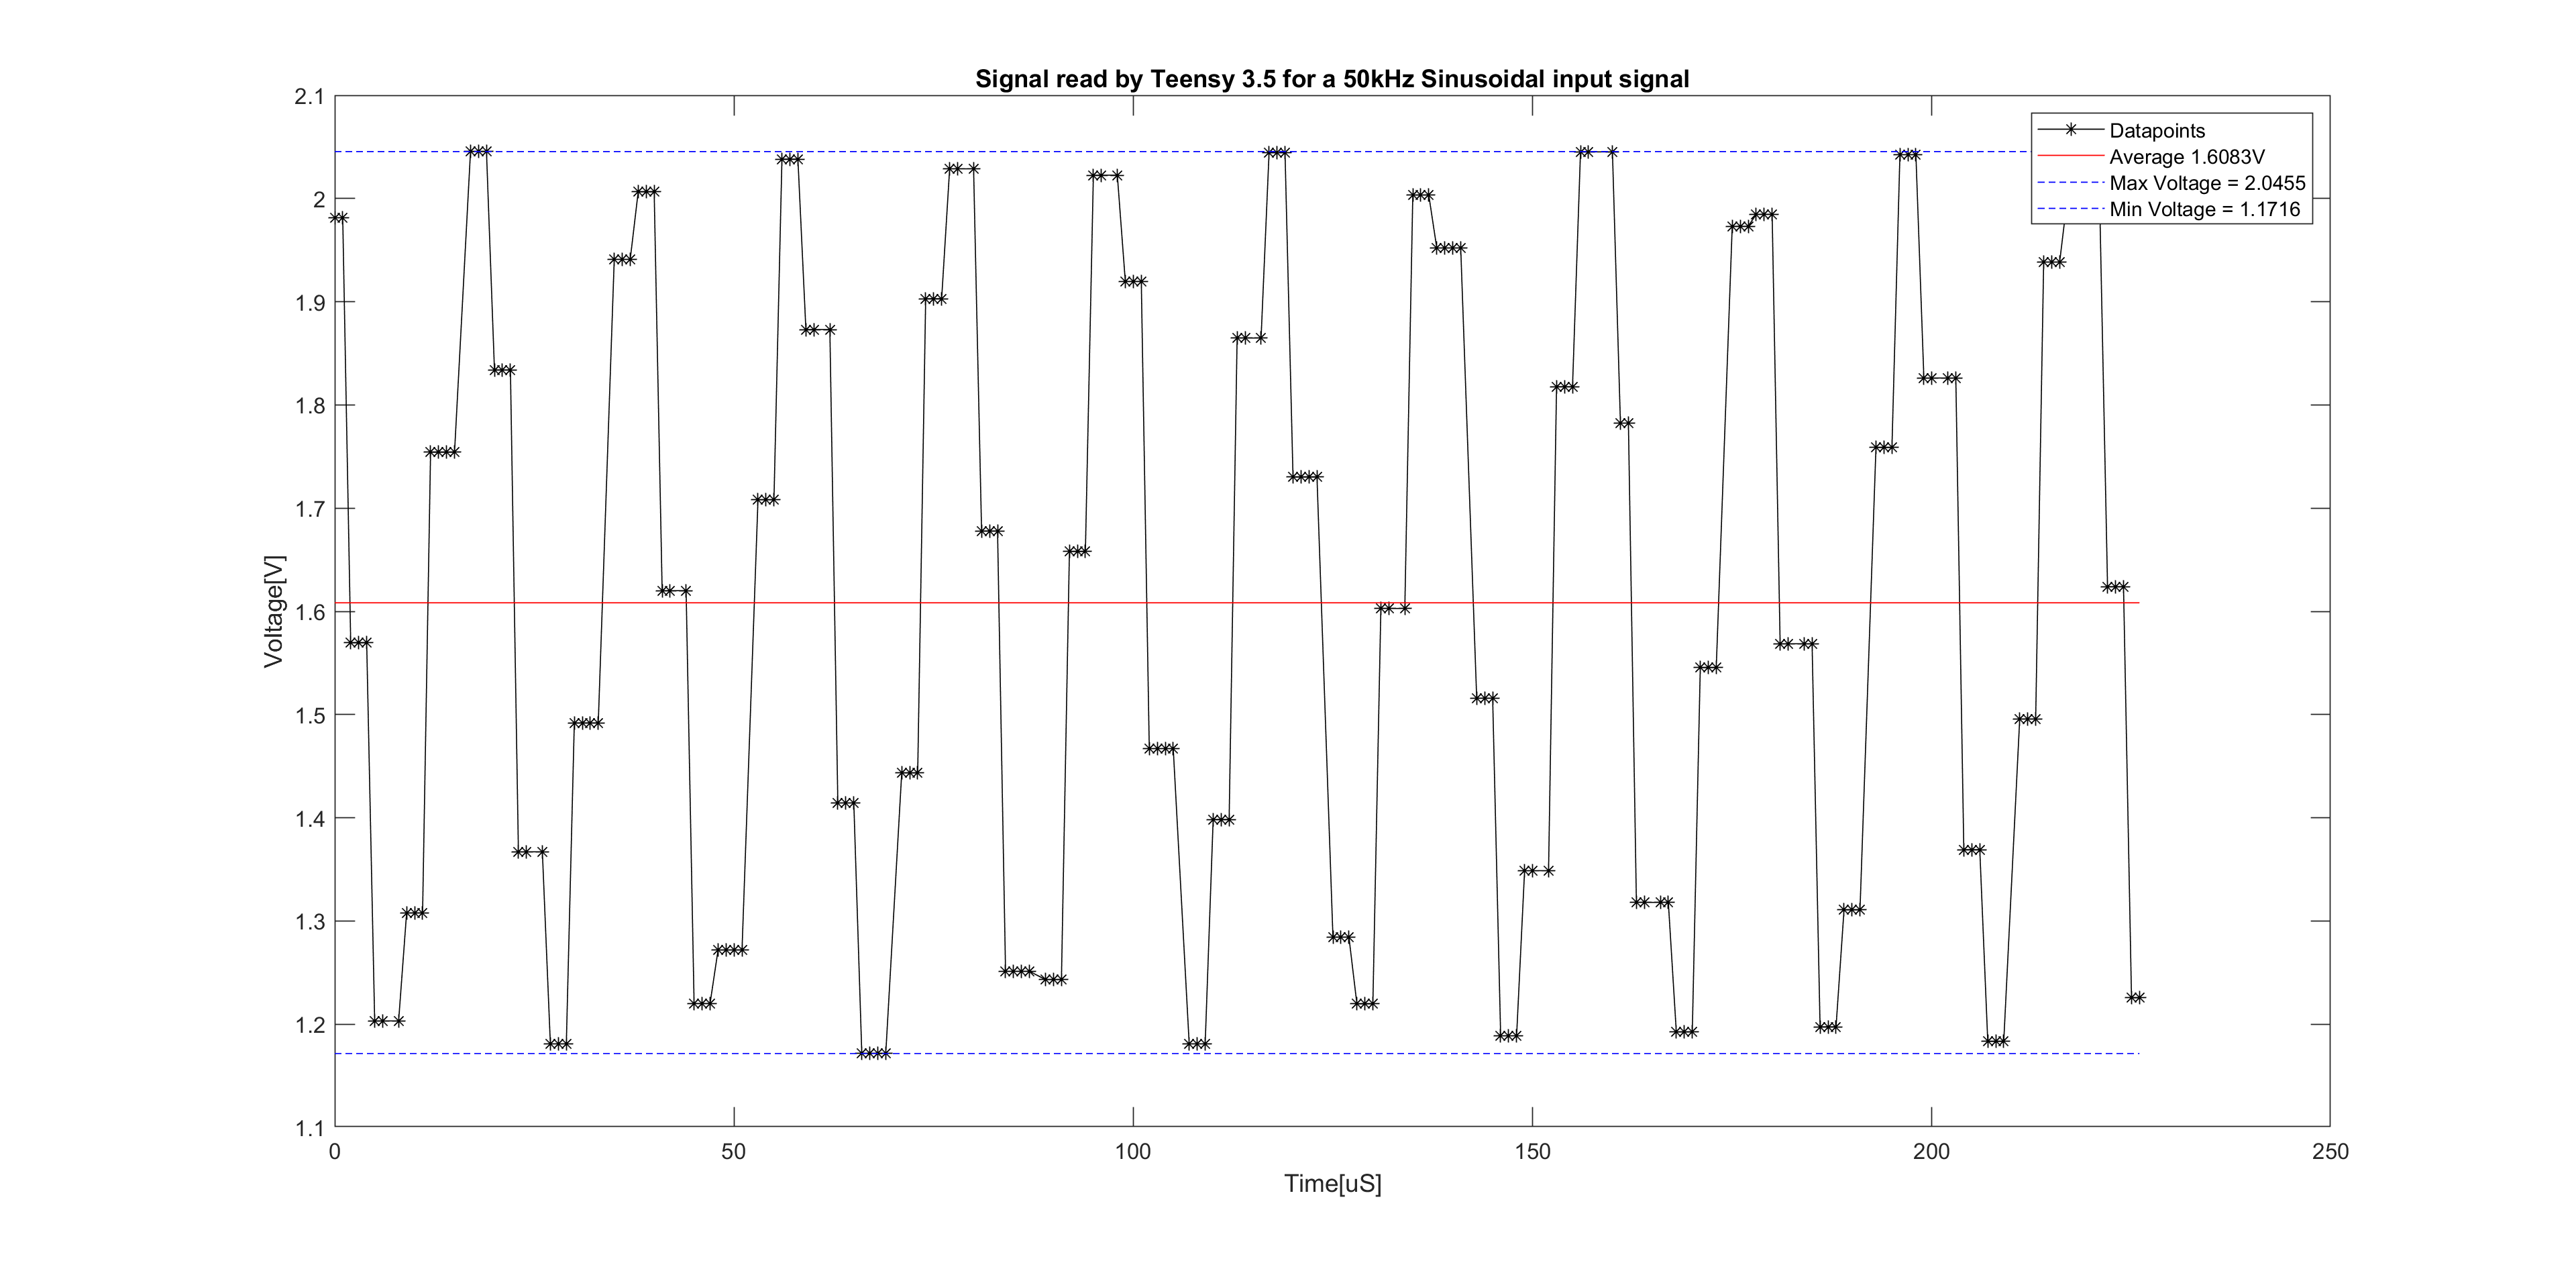
\includegraphics[width=0.50\textwidth,height=0.40\textwidth]{graphics/COntANalogResults.png}}
%    \label{fig:ContAnalSpeedREsults}
%    \hfill
%    \subfloat[\textbf{Sub figure caption }]{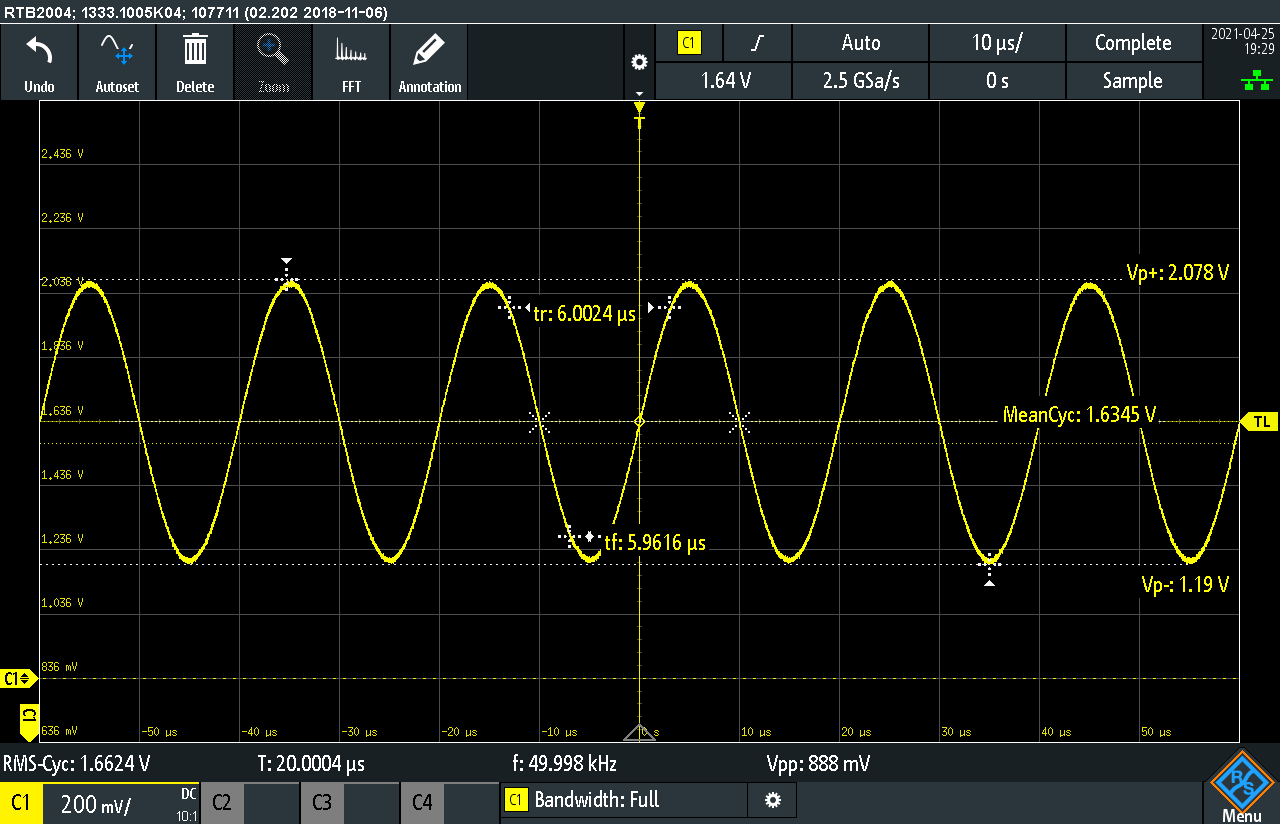
\includegraphics[width=0.40\textwidth,height=0.40\textwidth]{graphics/ContAnalogReadOscillascope.PNG}}
%    \label{fig:ContAnalOscillascope}
%    \caption{Results from the device compared to the oscilloscope readings}
%%\end{figure}


\subsection{PDBContinuousAnalogRead.ino}

PDBContinuousAnalogRead.ino utilizes three specific built-in peripherals on the Teensy 3.5 in order to read analog signals, which are the ADC, PDB and a DMA channel.
The PDB is an accurate timer that is used to trigger the ADC to do an analog to digital conversion.
Once each ADC conversion is complete DMA receives a trigger, the ADC value is then transferred using DMA to memory.
When initializing the DMA it needs to know a few things about the buffer to which the ADC value is being transferred to such as the size of the buffer and its address. 
This is important because DMA counts how many transfers have been made, and at a set number of transfers it triggers an ISR.
Since in this program the DMA buffer is a 2-dimensional array (2 by 256 to have each buffer 512 bytes in size).
The ISR is set to trigger when each of the buffers is full, meaning when the first buffer is full the ISR is triggered and its contents are moved to another storage buffer.
While that transfer is happening the destination address for the buffer was changed to the second buffer and the data transfer is continually happening while the first buffer is still transferring its contents to the storage buffer.
This is crucial in order to get a non-blocking code and not lose any data.
Therefore the speed of the program is dependent on how fast the Teensy can move data from the DMA buffer to the storage buffer.
The main program is then continually writing from the storage buffer to the SD card in 512-byte chunks.
A flowchart of the design and operation of the program can be seen in \textit{Figure~\ref{fig:CodeFlow}}.

\begin{figure}[h]
    \centering
    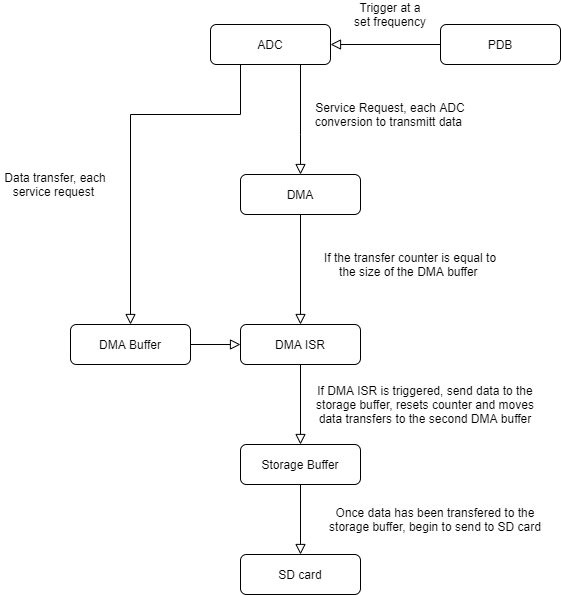
\includegraphics[width=0.70\textwidth]{graphics/flowChart.png}
    \caption{A flow chart giving a visual representation of the function of the program}
    \label{fig:CodeFlow}
\end{figure}


A more detailed explanation of setting registers can be seen in \textit{Appendix~\ref{sec:codeExplain}}.

\clearpage

\subsection{Testing}



%Skoða aftur á scopei færa langt frá trigger punknt ~50 sveiflur og skoða breytileika þar.
%skða líka með FFT
%Skoða með mismunandi söfnunartíðnum og bera saman og skoða powerið

%skoða innmerki  10k með 100k söfnunartíðni
%                20k með 200k söfnunartíðni
%                30k með 300k söfnunartíðni

%Hvað ég safna rétt í tíma
%hve mikið hljóð
%setja inn merki, mæla útmerkið með FFT á scopei.
%skoða hljóð frá generatornum og svo frá merkinu með fft
%sjá mynd, ef það koma eh suð toppar á fft frá bara generator, sjá hvort þeir detta niður með RC filter ef ekki þá er suðið að koma %frá kerfinu.



%\textbf{looking at the oscilloscope on the built-in led, triggering it to switch states each time ISR of the individual peripheral is %triggered. 
%Changing ISR only PDB = stable till sampleFreq  roughly 1MH  (491.7kHz)+- 0.3kHz measured by scope
%for 16 bits:
%ISR PDB ADC = stable till sampleFreq roughly 280kHz   (139.5kHz) +- 0.01kHz measured by scope
%whole system = stable till roughly 300khz samplefreq 
%Changing the resolution had minimal gains.
%It seemed to be able to be triggered a little bit faster however those were not stable for the Teensy and the program would crash.}

Multiple tests were performed on the device, all equipment used for the tests can be seen in the list below.
\begin{itemize}
    \item \textit{Rhode \& Schwarz RTB20004} digital oscilloscope with a 2.5 Gsps sampling rate for waveform confirmation.
    \item \textit{Rigol DG1022} waveform generator capable of generating signals up to 25MHz sine wave and a resolution of 1$\mu Hz$ and down to 2mVpp.
    \item \textit{Rigol DP831} programmable DC power supply.
\end{itemize}



\subsubsection{Frequency of PDB, ADC and the DMA}

Several tests were made in order to find the maximum frequency at which parts of the device could remain relatively stable.
These tests would use an ISR, triggered by either the PDB or the ADC.
The ISR would either turn on the built-in LED on the Teensy or turn it off, depending on whether the LED was on or off.
Which for every other ISR trigger would make the LED blink.
Three test cases were examined, first using just the PDB timer which would trigger the ISR. 
Secondly using the PDB and ADC together and finally for when the entire system was operational, for both cases the ISR would be triggered by the completion of an ADC conversion.
The setup of the test can be seen in \textit{Figure~\ref{fig:SetupCircSpeed}}, the oscilloscope was connected to the built-in LED, the Teensy3.5 was powered via USB and the op-amps were powered by the DC power supply.
The scope was set to take measurements of the time and frequency, which would be triggered by the rising edge of the rectangular signal that formed from blinking the LED. 
The oscilloscope shows the mean, maximum and minimum values for both frequency and time of each period.
The frequency measurements shown by the oscilloscope are actually halved since the scope counts the rising edge of the pulses and the time period measurement is double that of the actual trigger time.
As well as the cursor was set over a single pulse to show the actual frequency of the ISR trigger speed.
The measurements were stopped when the oscilloscope had made roughly 10k wave count.
The setup was the same for all three test cases.


\begin{figure}[h]
    \centering
    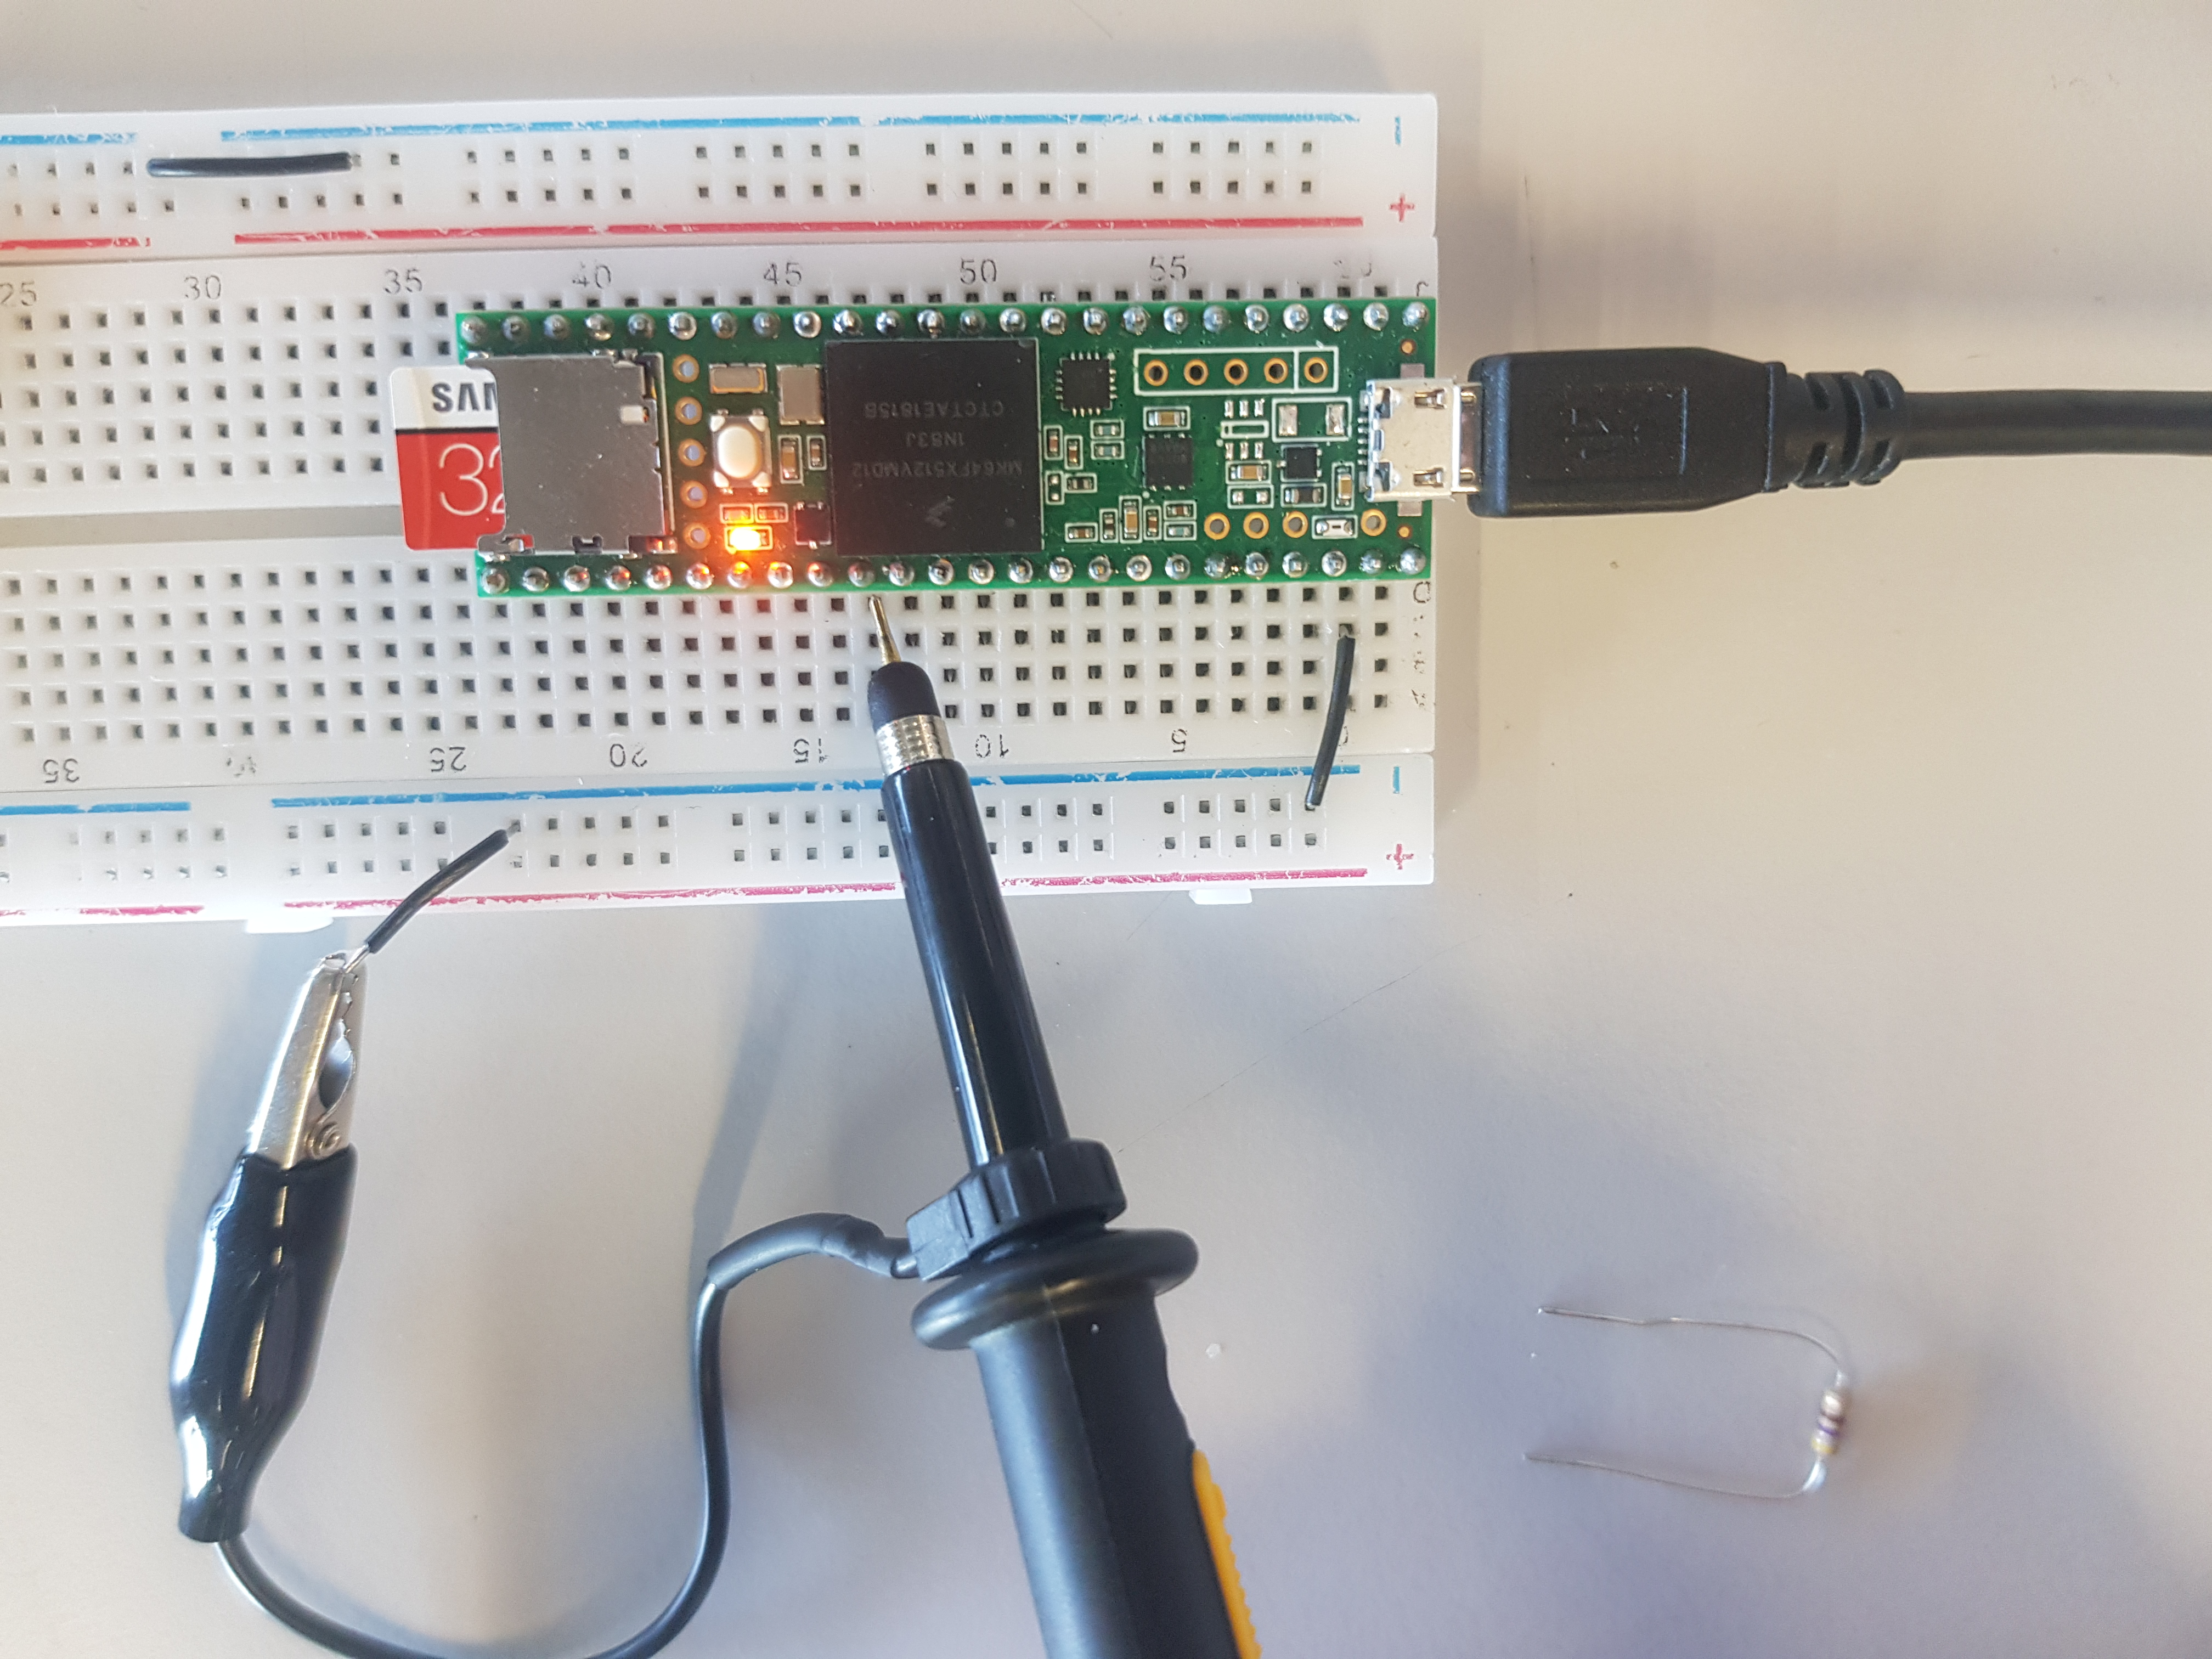
\includegraphics[width=0.7\textwidth]{graphics/SetupCircSpeed.jpg}
    \caption{The setup of the circuit for frequency for three test first just initializing the PDB, then the PDB and ADC and the third where the whole system was initialized.}
    \label{fig:SetupCircSpeed}
\end{figure}

In the first test, just the PDB timer was initialized and the ISR would trigger from the PDB timer.
Three set frequencies were tested, 1.2MHz, 600kHz and 300kHz.
The results of the tests can be seen in \textit{Figures~\ref{fig:PDBSp1200} - \ref{fig:PDBsp300}}.
The maximum frequency at which the PDB could run, was when the set frequency was set as 1.2MHz.
As explained before the actual frequency values from the oscilloscope are halved from the real values, so all measured frequency statistics are doubled, while the time of the period is halved.
The mean frequency was 1.17MHz, where the maximum was 1.27MHz and a minimum of 767.7kHz with a standard deviation of 27.1kHz. 
The mean time for a period was 852ns with a standard deviation of 27ns as seen in \textit{Figure~\ref{fig:PDBSp1200}}.

\clearpage

\begin{figure}[h]
    \centering
    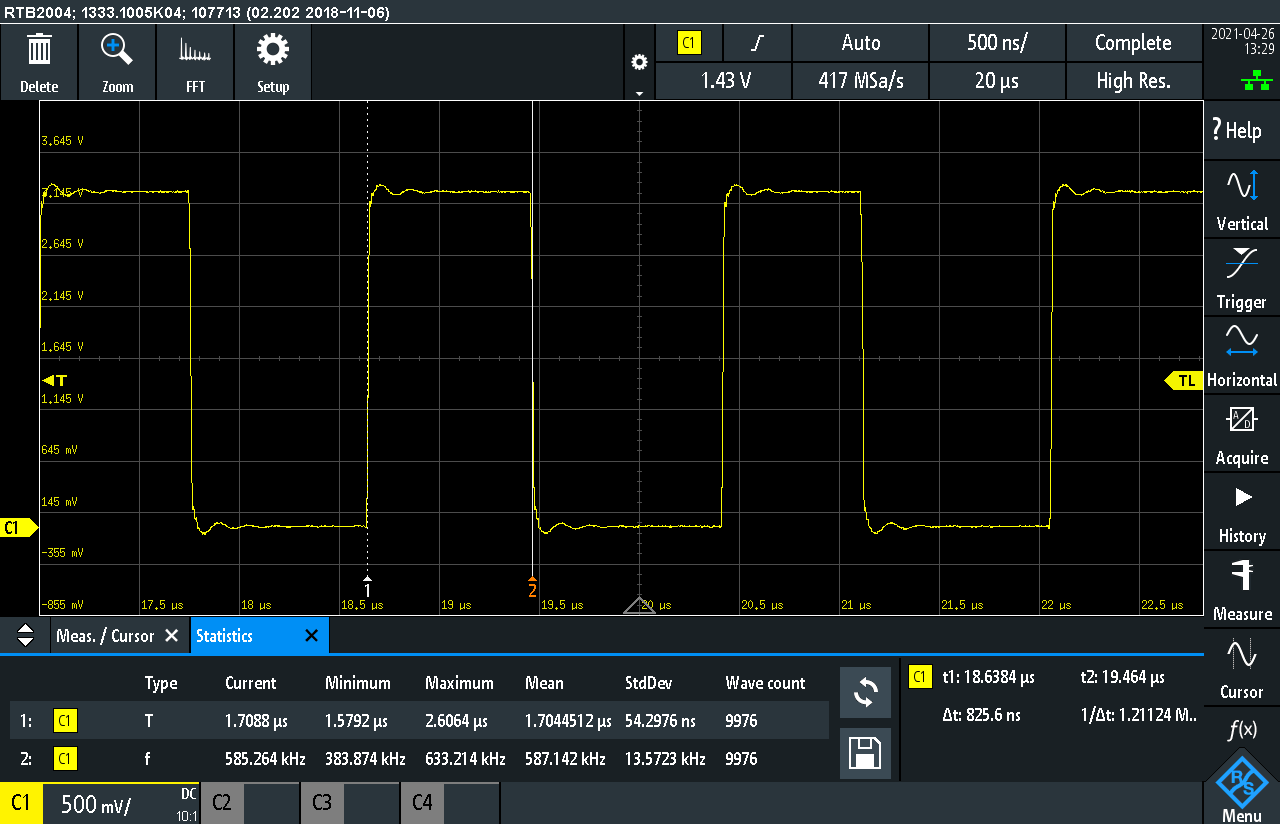
\includegraphics[width=0.8\textwidth]{graphics/STAT01_1200.PNG}
    \caption{The blinking of the LED, set frequency in the code was 1.2MHz}
    \label{fig:PDBSp1200}
\end{figure}

For the second test, the set frequency was 600kHz.
The mean frequency was 593.5kHz, where the maximum was 654.5kHz and a minimum of 470.7kHz with a standard deviation of 8.42kHz. 
The mean time for a period was 1.68$\mu$s with a standard deviation of 29ns as seen in \textit{Figure~\ref{fig:PDBSp600}}.

\begin{figure}[h]
    \centering
    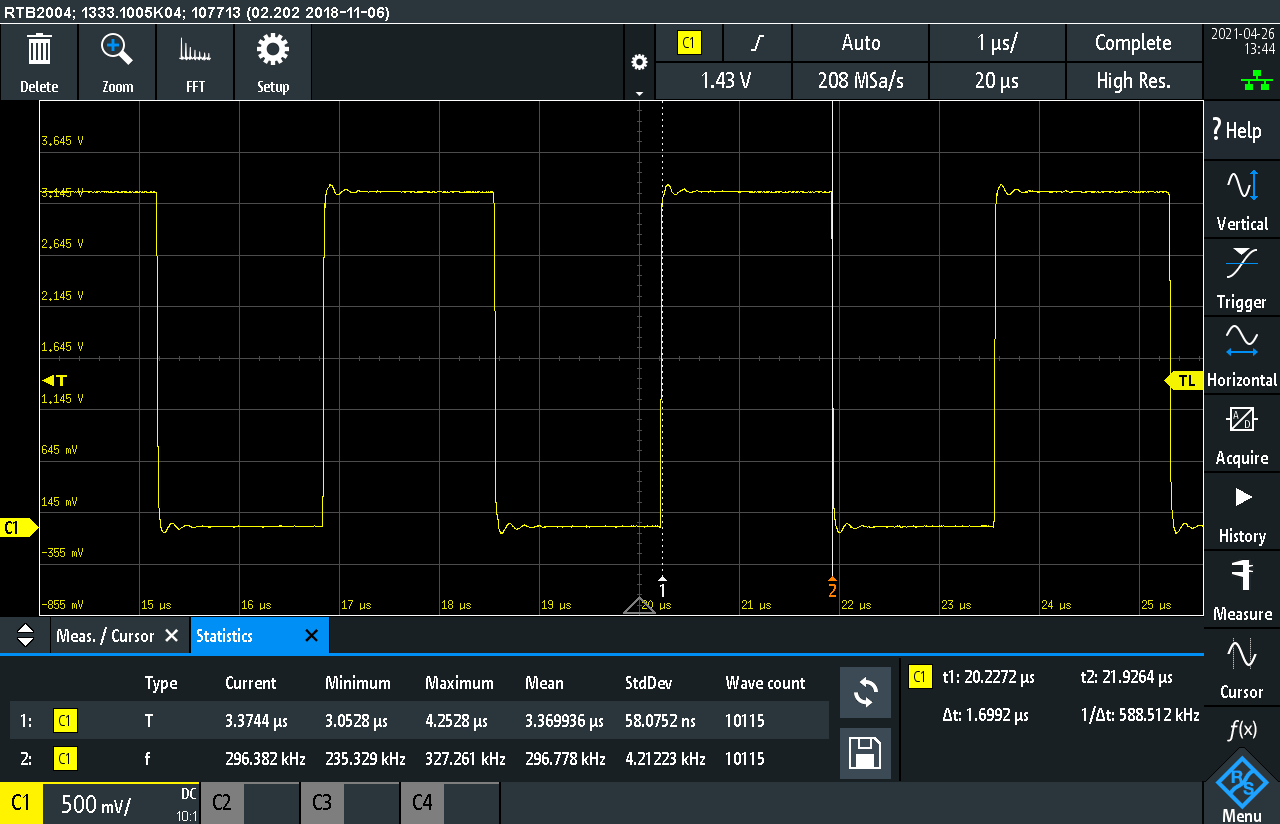
\includegraphics[width=0.8\textwidth]{graphics/STAT02_600.PNG}
    \caption{The blinking of the LED, set frequency in the code was 600kHz}
    \label{fig:PDBSp600}
\end{figure}

\clearpage

For the third test, the set frequency was 300kHz.
The mean frequency was 298.4kHz, where the maximum was 320.7kHz and a minimum of 122.4kHz with a standard deviation of 1.63kHz. 
The mean time for a period was 3.35$\mu$s with a standard deviation of 21ns as seen in \textit{Figure~\ref{fig:PDBsp300}}.


\begin{figure}[h]
    \centering
    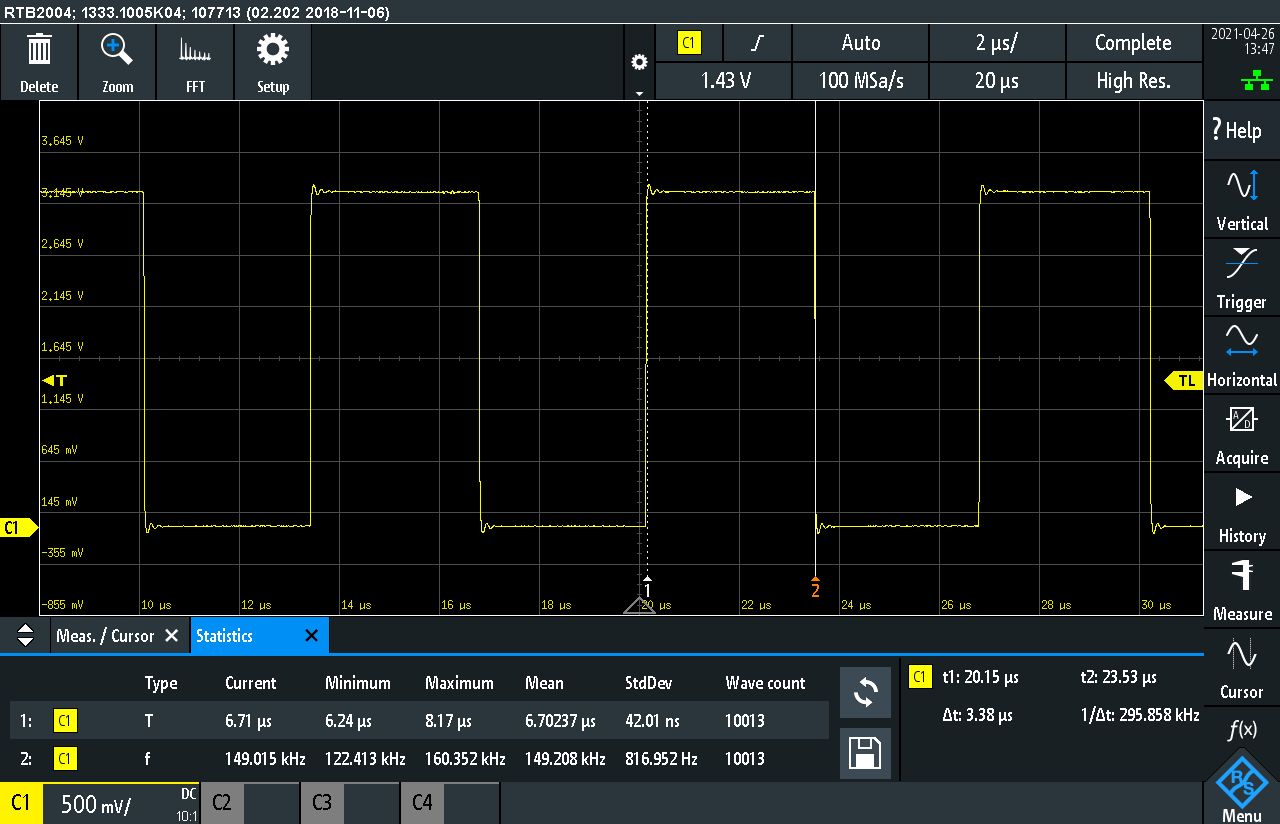
\includegraphics[width=0.8\textwidth]{graphics/STAT03_300.PNG}
    \caption{The blinking of the LED, set frequency in the code was 300kHz}
    \label{fig:PDBsp300}
\end{figure}


The next test was for the ADC, which used both the ADC and the PDB.
The ISR would also be set to trigger when completing an ADC conversion.
The set frequency was 280kHz, because at 300kHz the program would stop running after roughly 2 seconds.
The mean frequency was 279.1kHz, where the maximum was 208.3kHz and the minimum of 225.5kHz with a standard deviation of 1.1kHz. 
The mean time for a period was 3.58$\mu$s with a standard deviation of 14ns as seen in \textit{Figure~\ref{fig:PDBADCDMAsp280}}.

\clearpage

\begin{figure}[h]
    \centering
    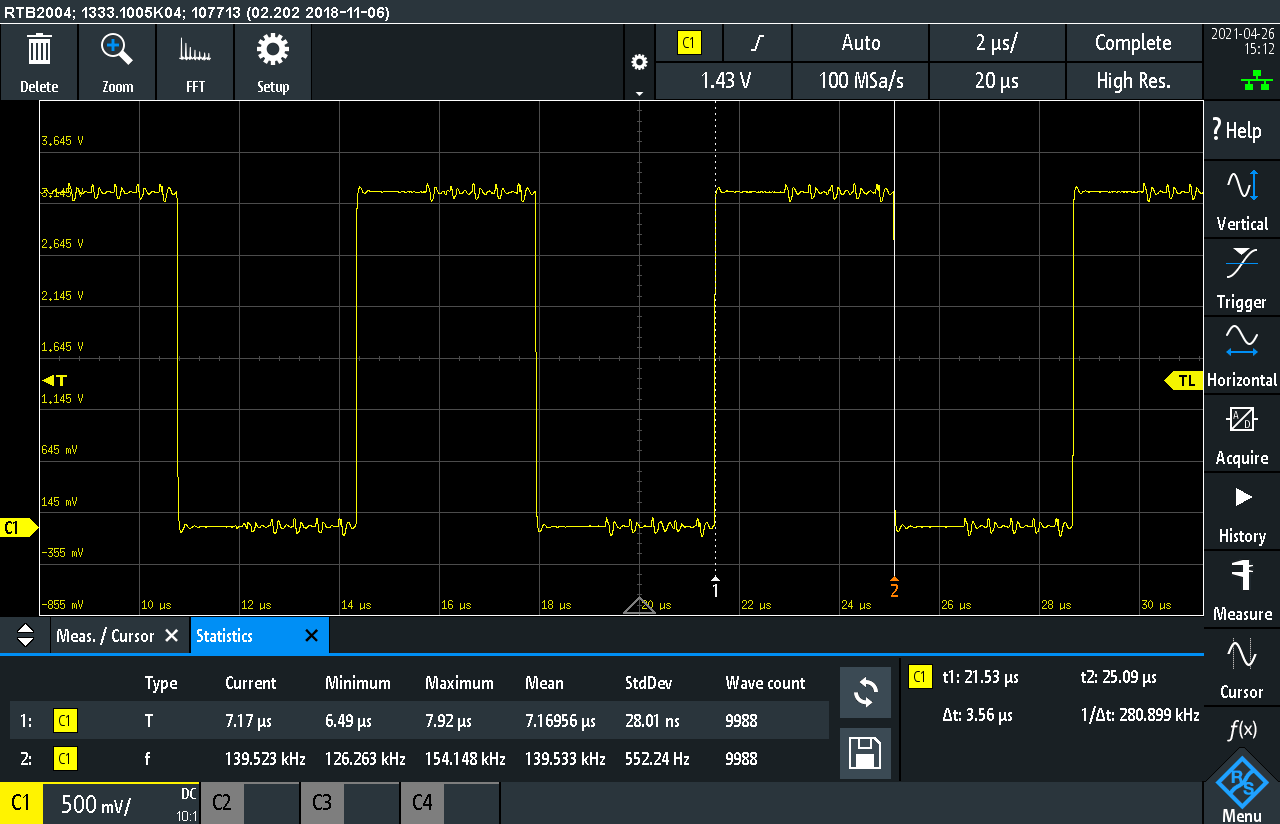
\includegraphics[width=0.8\textwidth]{graphics/STATADC_280.PNG}
    \caption{The blinking of the LED when completing an ADC conversion triggered the ISR, set frequency in the code was 280kHz}
    \label{fig:PDBADCDMAsp280}
\end{figure}

The next test was for the whole system was initialized, using the ADC, PDB and DMA.
The ISR is still set to trigger when completing an ADC conversion.
The mean frequency was 298.3kHz, where the maximum was 532.4kHz and a minimum of 208.5kHz with a standard deviation of 5.4kHz. 
The mean time for a period was 3.39$\mu$s with a standard deviation of 69.6ns as seen in \textit{Figure~\ref{fig:PDBADCDMAsp280}}.

\begin{figure}[h]
    \centering
    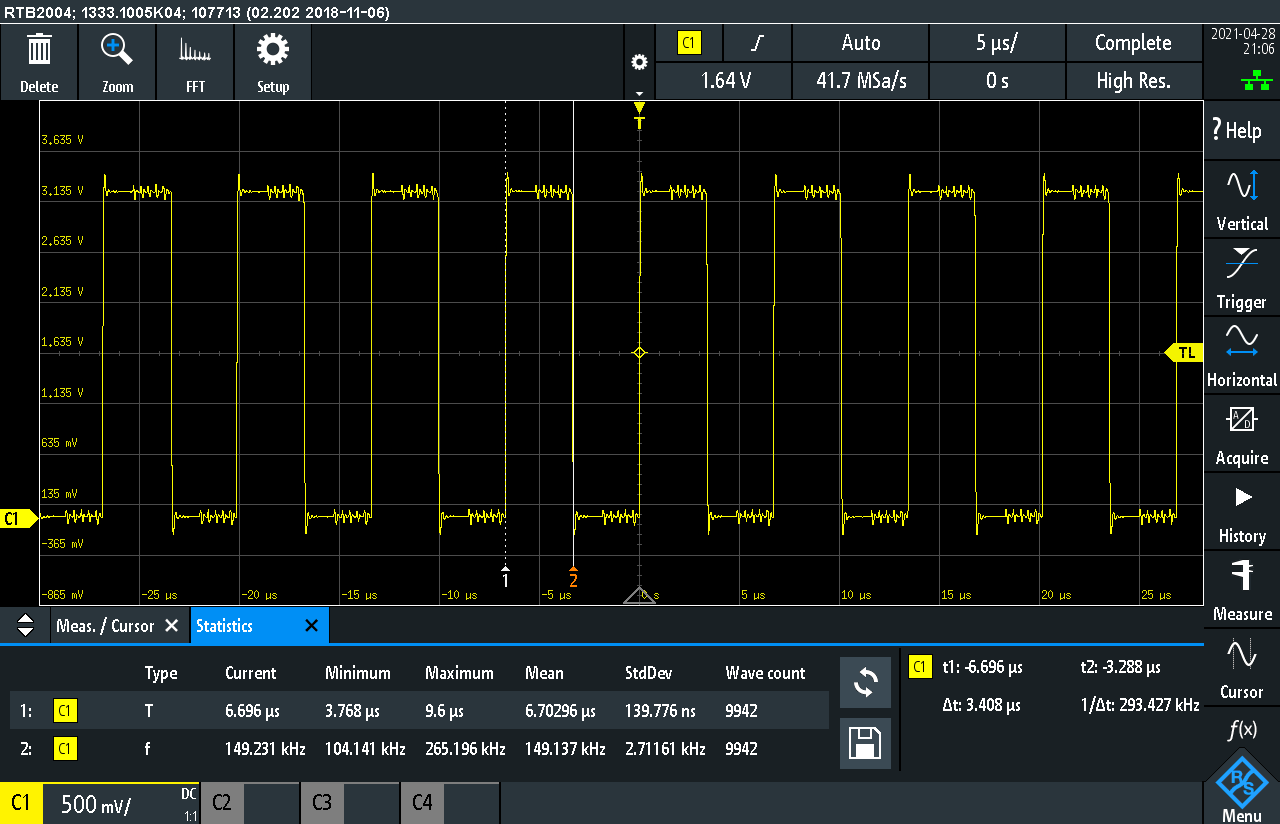
\includegraphics[width=0.8\textwidth]{graphics/ALLT300k.PNG}
    \caption{The blinking of the LED when completing an ADC conversion triggered the ISR, set frequency in the code was 300kHz}
    \label{fig:PDBADCDMAsp300}
\end{figure}





\subsubsection{Noise testing}

%setting https://picture.iczhiku.com/resource/eetop/SHkHEFiIIDHlSccB.pdf

Several tests were made in order to estimate the noise of the device.
The fast Fourier transform (FFT) function of the RTB2004 oscilloscope was used for the measurements and the DC power supply was used to power the op-amps.
The oscilloscope was set to AC coupled for the best broadband range measurement%https://training.ti.com/ti-precision-labs-op-amps-noise-measuring-system-noise 
, attenuator set to 1:1 ratio %https://www.testandmeasurementtips.com/reduce-oscilloscope-noise-measurements/
for accurate noise measurements and the Hannig FFT window was used.
Two test cases were examined, first when a sine wave was the input of the circuit and secondly when the input was connected to the ground and the probe connected to the output of the op-amps.
The setup for the tests can be seen in \textit{Figure~\ref{fig:SetupFFT}}.

%\textbf{%https://web.sonoma.edu/esee/courses/ee442/archives/sp2019/supp/defining_dBu.pdf
%- skoða} 
%https://www.youtube.com/watch?v=oLBGNC9FGwo&ab_channel=TexasInstruments minuta 3:47

\begin{figure}[h]
    \centering
    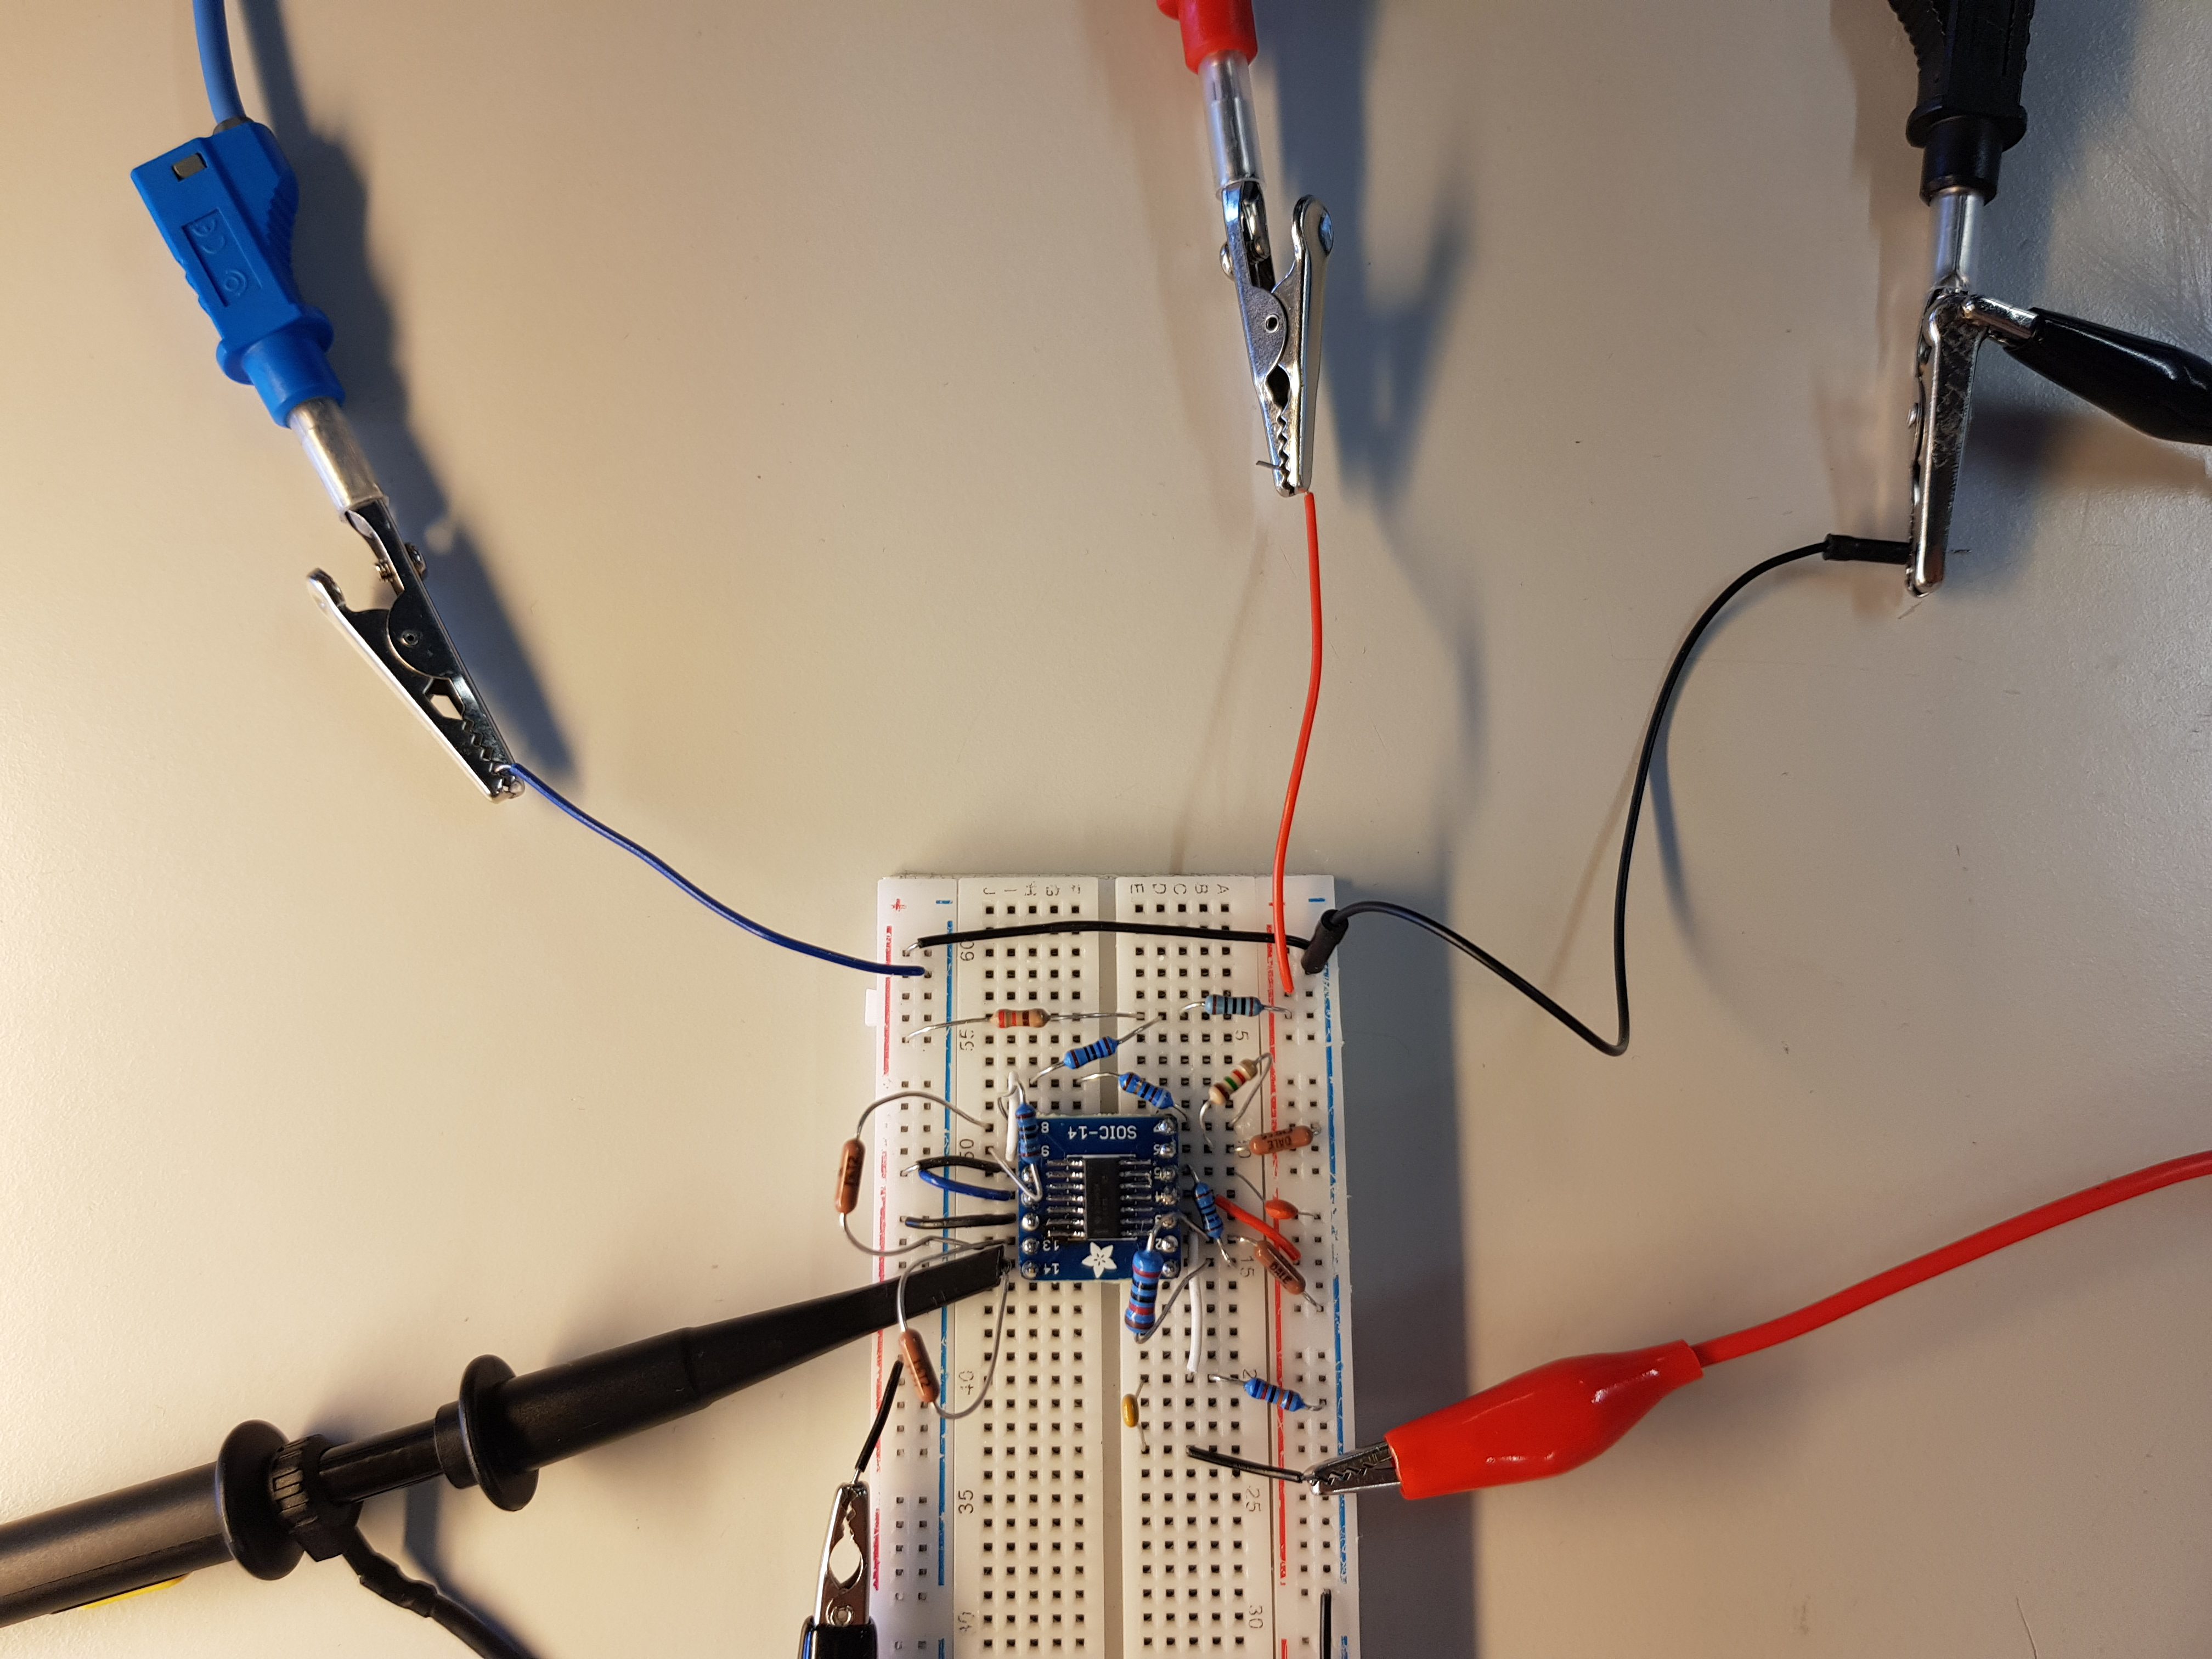
\includegraphics[width=0.7\textwidth]{graphics/TESTINGwSineinp.jpg}
    \caption{Configuration of the noise tests where the circuit is tested, where the probe is connected to the output of the op amps and the input signal is either a sine wave or its connected to ground.}
    \label{fig:SetupFFT}
\end{figure}


The bandwidth of the FFT was set at 100kHz with an input signal being a sine wave with 10$mV_{pp}$ and 20kHz frequency being sent to the input of the op-amps.
The results can be seen in \textit{Figure~\ref{fig:Noise20k10mVpp100kband}}, at 20kHz the input signal is apparent with a peak of 3dBm while the noise floor is around -72dBm.
Which yields a SNR, which is the difference between the two amplitudes as 75dB.

\clearpage

\begin{figure}[h]
    \centering
    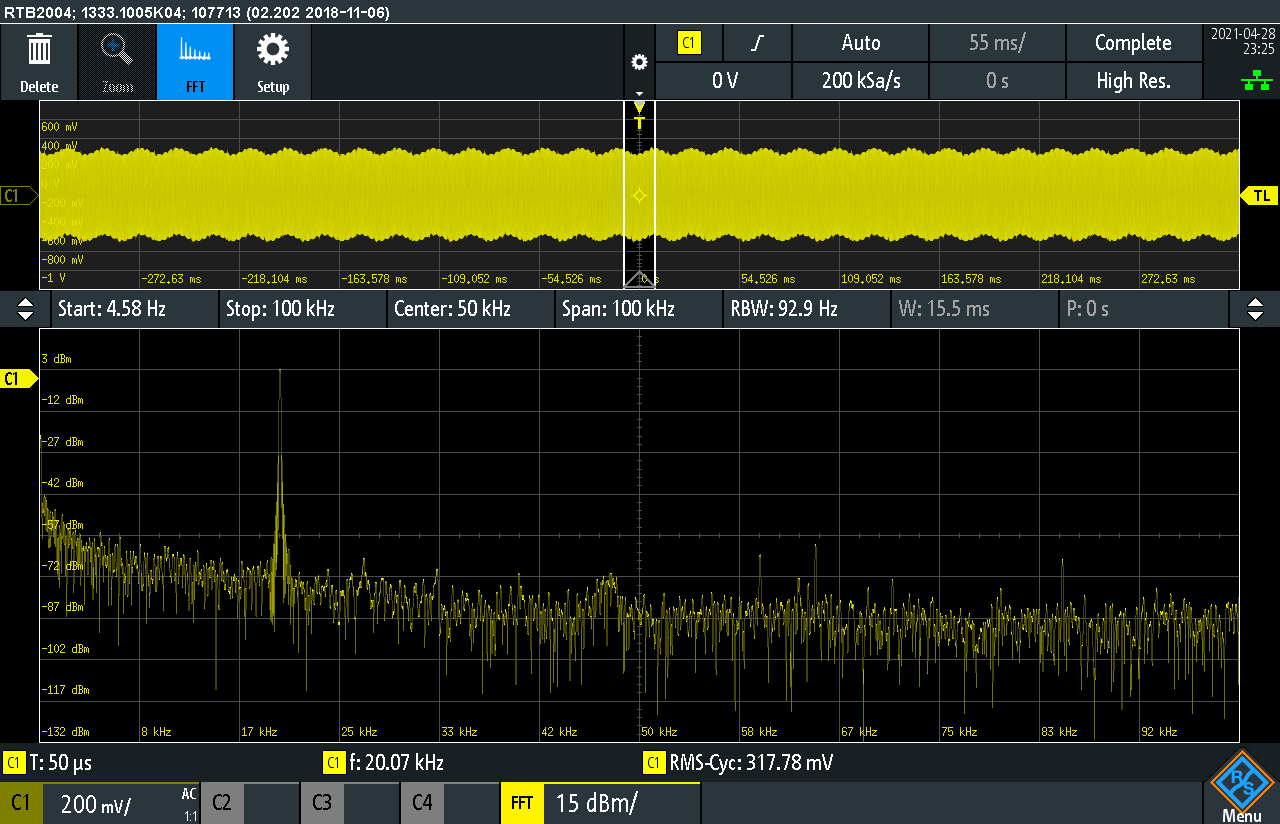
\includegraphics[width=0.7\textwidth]{graphics/Noise20k10mVpp100kband.PNG}
    \caption{FFT on the RTB2004 oscilloscope. An input sine wave signal of 10$mV_{pp}$ and a frequency of 20kHz.Top of the figure shows the output of the op amps and the respective FFT below it with a 100kHz bandwidth.}
    \label{fig:Noise20k10mVpp100kband}
\end{figure}



%\begin{figure}[h]
%    \centering
%    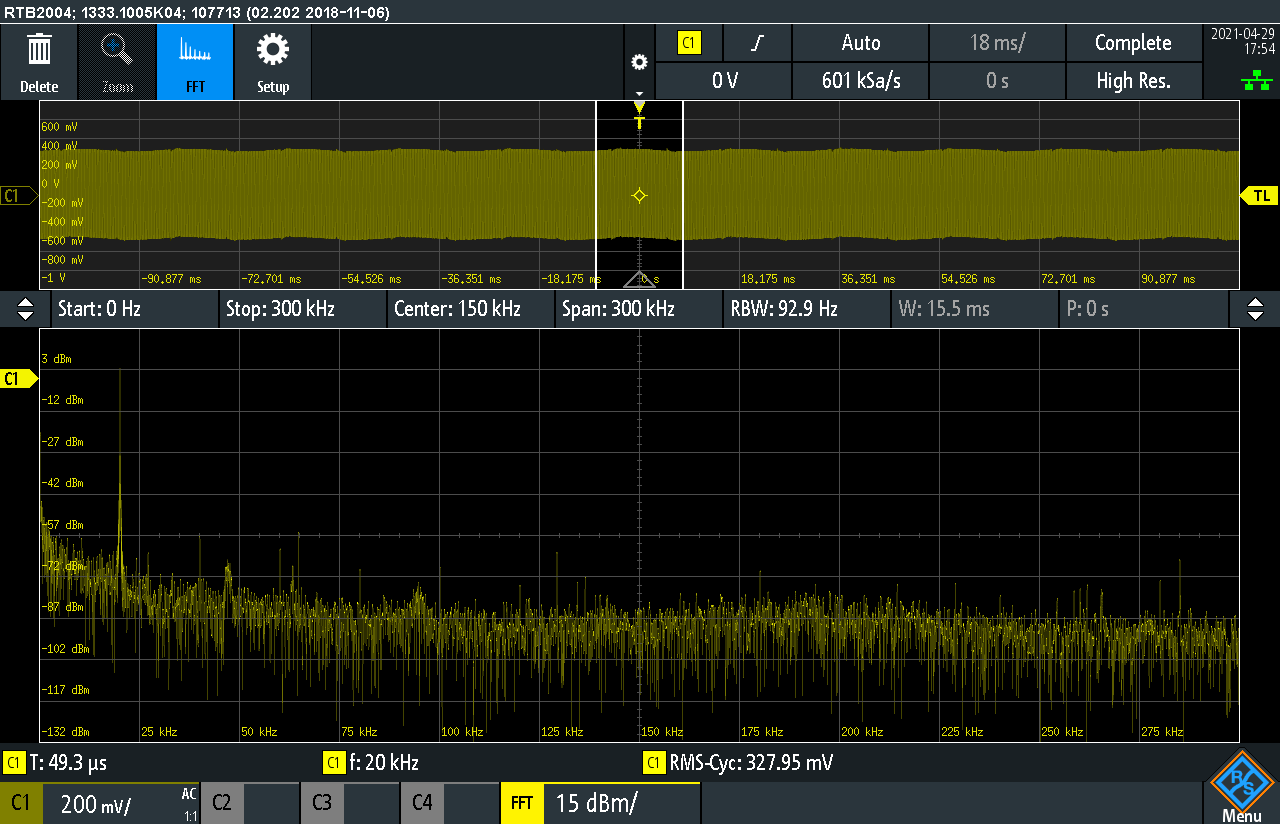
\includegraphics[width=0.7\textwidth]{graphics/Noise20kinp300kBand.PNG}
%    \caption{FFT on the RTB2004 oscilloscope. An input sine wave signal of 10$mV_{pp}$ and a frequency of 20kHz seen at the top of the figure and the respective FFT below it with a 300kHz bandwidth.}
%    \label{fig:Noise20k10mVpp300kband}
%\end{figure}


The same test was performed for just the generator, bypassing the op-amp circuit and connecting it directly to the oscilloscope.
The results can be seen in \textit{Figure~\ref{fig:NoiseGenerator20kInp100kBand}}, at 20kHz the input signal is apparent with a peak of -36.8dBm while the noise floor is around -116dBm.
Which yields a SNR of 80dB.

\begin{figure}[h]
    \centering
    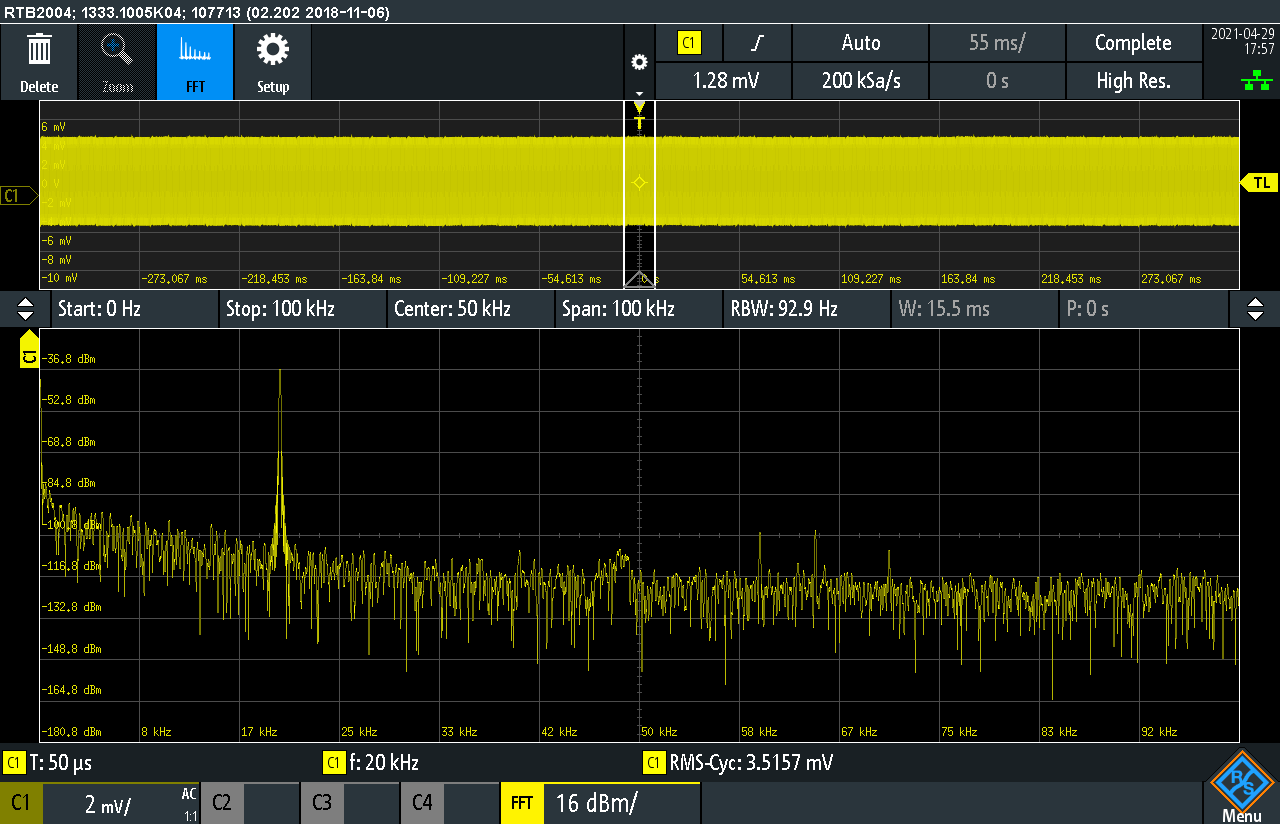
\includegraphics[width=0.7\textwidth]{graphics/NoiseGenerator20kInp100kBand.PNG}
    \caption{FFT on the RTB2004 oscilloscope connected directly to the signal generator. 
    An input sine wave signal of 10$mV_{pp}$ and a frequency of 20kHz seen at the top of the figure and the respective FFT below it with a 100kHz bandwidth.}
    \label{fig:NoiseGenerator20kInp100kBand}
\end{figure}

\clearpage

%\begin{figure}[h]
%    \centering
%    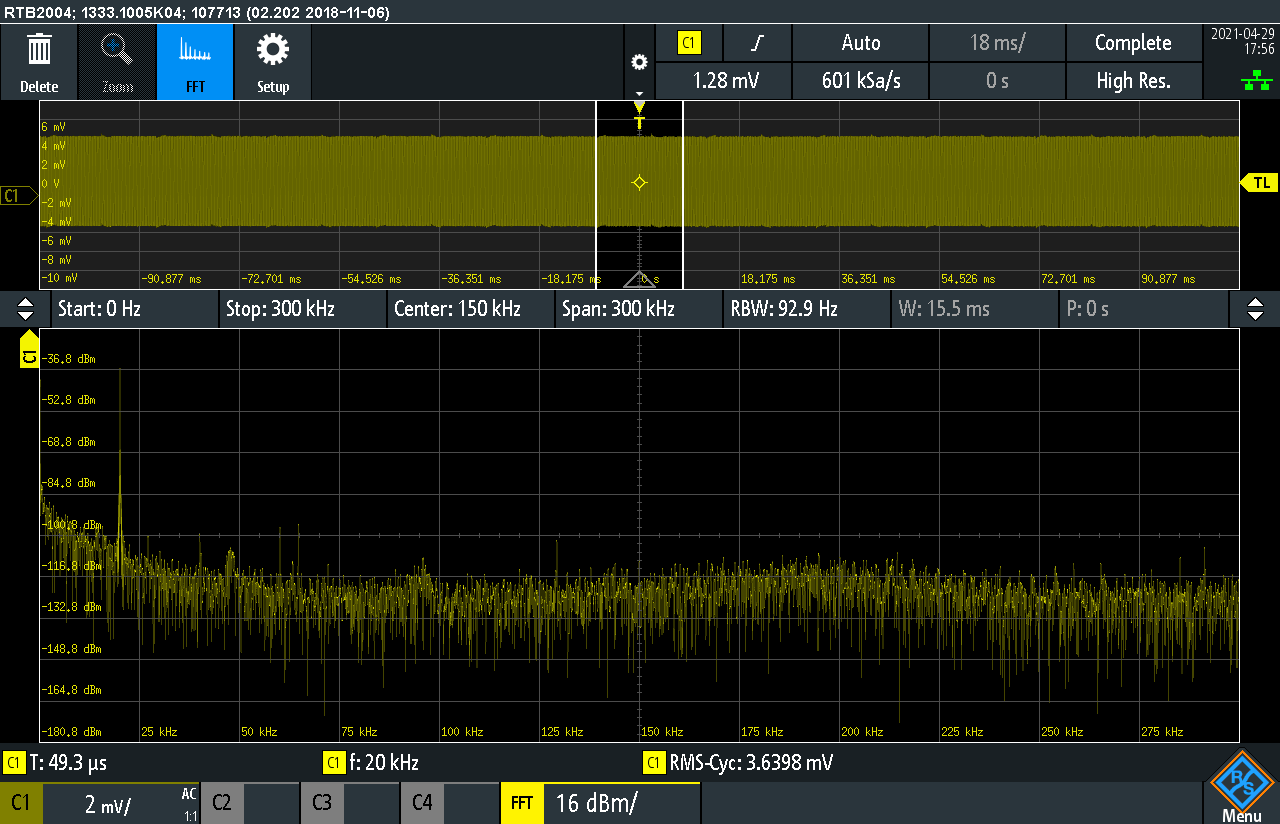
\includegraphics[width=0.7\textwidth]{graphics/NoiseGenerator20kInp300kBand.PNG}
%    \caption{FFT on the RTB2004 oscilloscope. 
%    An input sine wave signal of 10$mV_{pp}$ and a frequency of 20kHz seen at the top of the figure and the respective FFT below it with a 300kHz bandwidth.}
%    \label{fig:NoiseGenerator20kInp300kBand}
%\end{figure}


Now for when the input signal was connected to the ground.
The op-amps are still getting power from the DC power supply and the probe is connected to the output of the op-amps.
The results can be seen in \textit{Figure~\ref{fig:noisefloor100k}}.
This measurement yields a noise floor around of 87.1dBm.


\begin{figure}[h]
    \centering
    \includegraphics[width=0.7\textwidth]{graphics/NoiseFloor100k.PNG}
    \caption{General noise created by the circuit when op amps are powered and the input is grounded over a frequency band of 100kHz}
    \label{fig:noisefloor100k}
\end{figure}

%Now for when the bandwidth is set to 300kHz.
%Which can be seen in \textit{Figure~\ref{fig:noisefloor100k}}.
%This measurement yields a noise floor of around 86.8dBm.

%\begin{figure}[h]
%    \centering
%    \includegraphics[width=0.7\textwidth]{graphics/NoiseFloor300k.PNG}
%    \caption{General noise created by the circuit when op amps are powered and the input is grounded over a frequency band of 300kHz}
%    \label{fig:noisefloor300k}
%\end{figure}




\clearpage





\subsubsection{Recording signals from a generator}

All tests had the same setup of the device.
The Teensy3.5 was powered via USB, the probe was connected to where the input signal was being read and ground was connected to an analog reference of the Teensy3.5.
The op-amps were powered as before by a DC power supply and the input signal was generated by the waveform generator.
The setup of the device with everything connected can be seen in \textit{Figure~\ref{fig:testCircSetup}}.
The Teensy would record the signal to the SD card, where the values were in hexadecimal.
The output signal of the op-amps was then recorded by the RTB2004 oscilloscope.
Once it had stopped recording the data was transformed from hexadecimal to a decimal using the python script seen in \textit{Listing~\ref{src:converHex}} and then plotted using Matlab.


\begin{figure}[h]
    \centering
    \includegraphics[width=0.7\textwidth]{graphics/TestSetup.jpg}
    \caption{The setup for the circuit for the tests which used the wave form generator as the input signal.}
    \label{fig:testCircSetup}
\end{figure}

The following three tests are simulating a 170dB as a source level.
Using the Aquarian H1a as the hydrophone the voltage output would equate to  $V = 10^{170dB-190dB/10} = 10mV$, which was used for all the following tests.
The difference between the three tests was the input signals frequency and the sampling frequency of the Teensy.
The first test had the sampling frequency set at 100kHz and an input signal of 10kHz was used.
The data recorded by the Teensy can be seen in \textit{Figure~\ref{fig:Teensy10k100k}}.
While \textit{Figure~\ref{fig:Oscillo10k100k}} shows respective results from the RTB2004 oscilloscope.

\begin{figure}[h]
    \centering
    \includegraphics[width=1.0\textwidth]{graphics/10kin_100ksampl.png}
    \caption{Test of the circuit where the input signal was a sinusoidal wave with a frequency of 10kHz and an amplitude of $10mV_{pp}$ and the sample frequency was set as 100kHz}
    \label{fig:Teensy10k100k}
\end{figure}

\begin{figure}[h]
    \centering
    \includegraphics[width=0.7\textwidth]{graphics/10k10mvPP100ksamp.PNG}
    \caption{Shows the results of the oscilloscope scoping, where the probe was connected to the output of the op amp and the input signal was 10kHz.}
    \label{fig:Oscillo10k100k}
\end{figure}

\clearpage


Next the sampling frequency was increased to 200kHz and the input signal was 20kHz.
The results of the data recorded by the Teensy can be seen in\textit{Figure~\ref{fig:Teensy20k200k}}.
\textit{Figure~\ref{fig:Oscillo20k200k}} shows respective results from using the oscilloscope for the same input signal as before.

\begin{figure}[h]
    \centering
    \includegraphics[width=1.0\textwidth]{graphics/20kin_200ksampl.png}
    \caption{Test of the circuit where the input signal was a sinusoidal wave with a frequency of 20kHz and an amplitude of $10mV_{pp}$ and the sample frequency was set as 200kHz}
    \label{fig:Teensy20k200k}
\end{figure}

\begin{figure}[h]
    \centering
    \includegraphics[width=0.7\textwidth]{graphics/20k10mvPP200ksamp.PNG}
    \caption{Shows the results of the oscilloscope scoping, where the probe was connected to the output of the op amp and the input signal was 10kHz}
    \label{fig:Oscillo20k200k}
\end{figure}

\vspace{4cm}



In \textit{Figure~\ref{fig:Teensy30k300k}} the data that the Teensy recorded at 300kHz sample frequency, where the input signal was 30kHz.
\textit{Figure~\ref{fig:Oscillo30k300k}} shows respective results from using the oscilloscope for the same input signal as before.

\begin{figure}[h]
    \centering
    \includegraphics[width=1.0\textwidth]{graphics/30kin_300ksampl.png}
    \caption{Test of the circuit where the input signal was a sinusoidal wave with a frequency of 30kHz and an amplitude of $10mV_{pp}$ and the sample frequency was set as 300kHz}
    \label{fig:Teensy30k300k}
\end{figure}

\begin{figure}[h]
    \centering
    \includegraphics[width=0.7\textwidth]{graphics/30k10mvPP300ksamp.PNG}
    \caption{Shows the results of the oscilloscope scoping, where the probe was connected to the output of the op amp and the input signal was 30kHz}
    \label{fig:Oscillo30k300k}
\end{figure}

\fxfatal{Mögulega bæta við hraðamyndum með MB/s á öll test}


\clearpage


Two more tests were performed to better estimate the Teensys accuracy since at 10mV the signal generator was quite inconsistent and created some variance in its output. 
The test setup can be seen in \textit{Figure~\ref{fig:Last2TestsSetup}}, where the input signal bypasses the op-amp circuit and goes straight to the Teensy and Oscilloscope.

\begin{figure}[h]
    \centering
    \includegraphics[width=0.7\textwidth]{graphics/Last2Tests.jpg}
    \caption{The input signal connected to the 330$\Omega$ resistor straight to the Teensy.}
    \label{fig:Last2TestsSetup}
\end{figure}



The first signal was a sine wave with 1$V_{pp}$ and VDC offset of 1.65V and 50kHz frequency.
The data plotted from the Teensy can be seen in \textit{Figure~\ref{fig:OscilloCompTeensyAC}}.
Where the average from the Teensy data has an average voltage of 1.6462V, while the oscilloscope shows 1.6504V.


\clearpage


\begin{figure}[h]
    \centering
    \includegraphics[width=1.0\textwidth]{graphics/OscilloTeensyAC50k1vpp165voffpng.png}
    \caption{With a AC signal of 1$V_{pp}$ and 1.65V DC offset, Teensys readings at 300ksps compared to the RTB2004 oscilloscope at 2.5Gsps}
    \label{fig:OscilloCompTeensyAC}
\end{figure}

The second input signal was DC 1.65V.
The data plotted from the Teensy can be seen in \textit{Figure~\ref{fig:OscilloCompTeensyDC}}.
Where the average from the Teensy data has an average voltage of 1.6727V, while the oscilloscope shows 1.6695V.


\begin{figure}[h]
    \centering
    \includegraphics[width=1.0\textwidth]{graphics/OscilloTeensyDC165Read.png}
    \caption{With a DC signal of 1.65V, Teensys readings at 300ksps compared to the RTB2004 oscilloscope at 2.5Gsps}
    \label{fig:OscilloCompTeensyDC}
\end{figure}

%https://www.eevblog.com/forum/beginners/help-with-rapid-adc-data-aquizition/25/
%https://forum.pjrc.com/threads/30171-Reconfigure-ADC-via-a-DMA-transfer-to-allow-multiple-Channel-Acquisition?p=140300#post140300

%TESTa adc_dma_timer í arduino example segja hve hátt þett getur samplað.

%https://github.com/pedvide/ADC/blob/master/AnalogBufferDMA.cpp -> prufa þetta

%%% Local Variables: 
%%% mode: latex
%%% TeX-master: "DEGREE-NAME-YEAR"
%%% End: 
%%RUM: "Results"
\chapter{Discussion}

\section{Summary}

This thesis set out to look into the possibility of using a small, energy-efficient microcontroller to record cetacean vocalizations.
Different microcontrollers were explored and it was decided that the Tennsy was the best suited for the task.
Since it had a built-in ADC with 16bit resolution as well as an ADC library and even though not considered initially having DMA channels proved crucial to create the system.
An attempt was made to use the library however, that yielded poor results as seen in \textit{Figure~\ref{fig:ContAnalREsults}}. 
It would record a conversion even though the ADC was not ready for a new conversion.
So a decision was made to directly set the registers.
The final system operates by having a PDB timer trigger the ADC at precise intervals, and a DMA channel takes the data to memory where it can later be sent to the SD card.

Aquarian H1A hydrophone sets some recommendations for the preamplifier circuit. 
Such as the gain for cetacean monitoring (40dB gain ) as well as the maximum frequency of 100kHz, which can be seen in \textit{Section~\ref{sec:AquarionHydro}}.
The preamplifier was designed with that in mind and in \textit{Section~\ref{sec:CircResult}}, there it is shown that for both the gain required, as well as filtering signals that are not within the bandwidth of the hydrophones sensing abilities.

Several tests were made to assess the capabilities of the final device.
The first tests were regarding the capabilities of the PDB timer and its capability to trigger at a set frequency.
It is able to be triggered as fast as 1.2MHz.
However that is out of the ADC specs.
The system is able to run at 300kHz sampling frequency, with a sampling jitter of 69.6ns.
Which is insufficient for 16bits \fxfatal{SPurja baldur} %in order to maintain a 0.5LSB standard deviation.
%http://www.audiophilleo.com/zh_hk/docs/Dunn-AP-tn23.pdf - sampling jitter

Several noise tests were performed on both the entire device as well as the signal generator.
There was no special shielding used and the ground for the probe could act as an antenna these factors could all attribute to some extrinsic noise generation.
How ever in \textit{Figure~\ref{fig:Noise20k10mVpp100kband}} shows that an input signal of nominal value is not lost in noise, with a 75dB SNR which is more than sufficient as \textit{section~\ref{sec:DigitalAudiRec}} demonstrates.

Three tests were performed on the whole device where the input signal to the op-amps was a sine wave with a different frequency and for each test the sampling frequency was changed to be 10x that of the input signal.
This was done to see if the device was actually capable of 300kHz sampling.
In \textit{Figures~\ref{fig:Teensy10k100k},\ref{fig:Teensy20k200k} and~\ref{fig:Teensy30k300k}} the recorded results can be seen.
The device appears to be capable of sampling up to 300kHz, where it follows each signal nicely and has 10 data points for each period.

Two more similar tests were performed, since at 10$mV_{pp}$ the signal had a lot of variation compared to the actual signal, which could cause some errors.
So two more tests were performed, where the input signal was connected directly to the Teensy through a resistor.
Two signals were tested, first with a sine wave with a voltage offset of 1.65V, 1$V_{pp}$ so that the Teensy would not receive negative voltages and a frequency of 50kHz.
The comparison between the results from the Teensy compared to what the oscilloscope received can be seen in \textit{Figure~\ref{fig:OscilloCompTeensyAC}}.
The same test was performed with a DC 1.65V, the results can be seen in \textit{Figure~\ref{fig:OscilloCompTeensyAC}}. 
The results are quite good, the Teensy is clearly able to keep up with the signal and give accurate results.
There is a difference between the mean, maximum and minimum voltages. 
But that could be the results of not being exactly taken at the same time as well as the oscilloscope samples at a much higher rate which could influence the outcome.


\clearpage


\section{Conclusion}\label{sec:conclusions}

Currently the device is still in prototype stages where it is still on a breadboard and has yet to be proven with a hydrophone.

The preamplifier circuit is configured to have the Aquarian H1a hydrophone as its source for signal sensing, which can easily be replaced with a different one.
The bandwidth of signals can also be altered easily by changing the high- and low pass filter setup.
Since dominant frequencies of cetacean vocalizations of whales found near Iceland seem to be under 30kHz.
It also consumes very little power, where the op-amps in total need around 0.165W and the Teensy draws 0.25W so in total the total power consumption should be around 0.415W which is way under the requirements.
So in total the device consumes roughly 0.415W at 3.3V, which is way under the requirements set at the start.
The current configuration of the project costs around 190\$ with the hydrophone, op-amps and the Teensy3.5.
It is hard to find a price for a complete system capable of recording cetacean vocalization but considering that devices such as the RUDAR uses the CRT C57 hydrophone which costs around 1290€.
It is safe to say the total cost of the recording device is low cost relative to other products commercially available.

The device is currently capable of recording continuously at 300ksps for 16bit resolution, which in theory should be more than sufficient to record signals up to 150kHz according to the Nyquist-Shannon theorem.

It was however decided early on to see the maximum potential of the Teensy platform audio recording and see its capabilities, which can then beneficial to the researchers.
Because some research suggested vocalization occurring at higher frequencies as well as the echolocation noise can go well above 100kHz so the device could record at least some parts of those.

\fxfatal{Tala við Baldur um sampling jitter, breyta ef þarf og tengja project goals aðeins meira eins og þyngd og lengd tímans sem það getur verið út á hafi}
In the end, the thesis shows that the Teensy platform is more than capable for the task of recording cetacean vocalizations.
As human civilization grows and expands it impacts animal wildlife more and more, whether that be land- or water creatures.
Creating different ways as well as improving current methods to monitor those effects on the animals.
Becomes ever so more crucial, in an effort of ensuring the survival of some species and will contribute to a future where human impact on both the earth and wildlife is hopefully decreased to a point that is sustainable.

%%% Local Variables: 
%%% mode: latex
%%% TeX-master: "DEGREE-NAME-YEAR"
%%% End: 
%%RUM: "Discussion"







%% ---------------------------------------------------------------
\printbibliography{} %%RUM: "References"

%% If appendices are needed, uncomment the following line
%% and include the appendices in separate files
\appendix{}%%RUM: "Appendicies (as appropriate)
\chapter{Setting of the registers}\label{sec:codeExplain}
\fxfatal{Eitthvað að kikja á }
To configure Teensy's ADC, DMA, PDB, the datasheet of the Kinetis K64F reference manual was used \cite{freescale_semiconductor_kinetis_2021}.
The information regarding the registers of each module can be found among other things.

%\textbf{BLS 933 \cite{freescale_semiconductor_kinetis_2021}.}
Starting with the PDB  which can be seen in \textit{Listing \textbf{BÆTA VIÐ kóða}}.
Firstly the clock for the PDB clock needs to be enabled, which is done by setting the SIM\_SCGC6\_PDB;
Which for the Teensy3.5 is 60MHz default and can be scaled down using prescaler.
Since the desire was to trigger at a high frequency the prescaler and multiplier of the prescaler were both set as 1 for the high clock speed possible.
\textbf{$$input clock = \frac{F\_BUS}{\frac{prescaler}{/multiplier}} = 60MHz$$}
Then the modulus register needs to be set, which will define the frequency of which the PDB will trigger and was calculated using the equation below.

$$modulus = \frac{input clock}{sample frequency}$$

The input clock increases a counter at the rate of its speed and the modulus sets the value of which the counter will set at zero and restart its count if the PDB is in continuous mode.
Once the modulus has been determined, several registers need to be configured in order to define the PBDs operation.
Most of which is done via PDB0\_SC register, which is the status and control register for PDB on channel 0.
Firstly to enable the PDB $ PDB\_SC\_PDBEN $ is set.
Then the trigger input source is selected as software trigger, by selecting $0xf (15)$ in $ PDB\_SC\_TRGSEL $.
To have to PDB run until it is stopped, the continuous mode needs to be enabled which is done by enabling $ PDB\_SC\_CONT $.
The PDB can trigger an interrupt to do that PDB interrupts need to be enabled, which is done by enabling
$ PDB\_SC\_PDBIE $.
There needs to be set an interrupt delay when using the PDB for the interrupt, which is done by setting a value to $PDB0\_IDLY = 1;$ and the ISR is triggered when the PDB counter reaches idly value.
Once the PDB configuration has been set, the registers need to be updated which is done by $ PDB\_SC\_LDOK$.
Then a PDB pre-trigger needs to be enabled since it is used to precondition the ADC block prior to the actual ADC conversion occurs.
%\textbf{p942}
This is done by enabling the pre-trigger by enabling the $PDB0\_CH0C1\_EN$ as well as the channel pre-trigger output $PDB0\_CH0C1\_TOS$.
This is achieved by writing $0x101$ to PDB0\_CH0C1.
%\begin{figure}[h]
%    \centering
%    \includegraphics[width=0.70\textwidth]{graphics/PDBtrigger.png}
%    \caption{PDB ADC triggers and DAC interval triggers use case \textbf{KANSKI sleppa nennei ekki að tala um}\cite{freescale_semiconductor_kinetis_2021}}
%    \label{fig:PDBTrigger}
%\end{figure}
Then the ADC can be configured first, the conversion mode needs to be determined.
The built-in ADC is up to 16bit and can be configured to run at 8-, 10-, 12- and 16-bit resolution modes, which is done through $ADC\_CFG1\_MODE$.
Two different reference voltages can be set, for the configuration of the circuit analog ground pin is used instead of an internal ground.
To achieve this $ADC0\_SC2$ needs to be set to 0.
Since the ADC is supposed to PDB trigger, that needs to be enabled.
$ADC\_SC2\_ADTRG$ sets the ADC to be hardware triggered, which in this case is set to be the PDB.
DMA transfer needs to be enabled here so that the conversion values of the ADC can go straight to memory, which is done by enabling  $ADC\_SC2\_DMAEN$.
All that is left is to select the analog pin, which is done by writing the pin hex value to $ADC0\_SC1A$ which in this case was "A9" or 0x04, see page 120 in \cite{freescale_semiconductor_kinetis_2021}.
The results of each conversion are then stored in $ADC0\_RA$ data result register.

Lastly the DMA is configured, to help with the process "DMAChannel.h" was used, which is a Teensy library.
Multiple registers need to be configured and set.
For instance where the data is coming from, where it is supposed to be delivered and when to go into the interrupt service routine (ISR) to name a few.
To initiate a DMA channel DMA.begin() is called.
Then the trigger for when the DMA transfer is supposed to occur needs to be set, which is done by setting the service request trigger as when an ADC conversion occurs.
This is done by configuring the $dma.triggerAtHardwareEvent$ as seen here $dma.triggerAtHardwareEvent(DMAMUX\_SOURCE\_ADC0)$.
Which sets in motion the DMA transfer.
Defining the source address $dma.TCD->SADDR$ needs to be set in this case, the location of the results of the ADC conversion, $ADC0\_RA$.
If the source address changes between each DMA transfer, there needs to be an offset put on the address which is done via $dma.TCD->SOFF$. 
Which in this case is 0 bytes, since $ADC0\_RA$ is just overwritten for each ADC conversion and its address does not change.
If the source address changes between each ISR call then adjustments can be made through $dma.TCD->SLAST$, which also does not change and is still the address of $ADC0\_RA$.
The data that is incoming and supposed to be transmitted needs to be set, which in this project is 2 bytes since the ADC will be configured in an above 8bit resolution.
This is done by $dma.TCD->ATTR = DMA\_TCD\_ATTR\_SSIZE(1) | DMA\_TCD\_ATTR\_DSIZE(1);$ which defines 16bit data transfers.
Which firstly defines the size of the incoming data as well as defining the destination data transfer size.
The number of bytes to transfer for each service request $DMAMUX\_SOURCE\_ADC0$ which is done with  $dma.TCD->NBYTES_MLNO = 2;$, this is considered a minor loop .
Then the destination source needs to be set like before, $dma.TCD->DADDR = dmaBuf;$ defines the destination address to a DMA buffer called dmaBuf which is defined in the main program.
This time there needs to be an offset is set to the address since the DMA is writing to a buffer to store the value instead of just overwriting the value like it was for the source.
This is done by setting the destination offset as the size of the ADC conversion value, or 2 bytes $dma.TCD->DOFF = 2;$.
To keep track of how many values have been set through DMA, the  $dma.TCD->CITER\_ELINKNO $ counter is set as the size of the buffer that the DMA values are being transferred to.
This value is decremented each time a value has been transferred via service request and transfer.
Since in the main program dmaBuf is 2 arrays of a size of 128 indexes this is set to 128 \textbf{Staðfesta!}.
When the count reaches 0, meaning the DMA buffer is full.
The counter needs to be reset back to its original value, this is done by setting $dma.TCD->BITER\_ELINKNO$ as the same value as the counter was set as.
The destination of the last address adjustment for the next transfer needs to be set, which is done by $dma.TCD->DLASTSGA = -sizeof(dmaBuf);$
When both DMA buffers are full, DMA resets, so it can rewrite to the first buffer.
To define when the ISR occurs, the $dma.TCD->CSR $ is set.
Since the BITER register was also set the reference manual states to use $DMA\_TCD\_CSR\_INTMAJOR$, however this resulted in only half the data being transmitted so $DMA\_TCD\_CSR\_INTMINOR$ was also set.
This sets DMA to trigger twice once when the first DMA buffer is full as well as when the second buffer is full.

Finally the DMA channel is enabled by $dma.enable();$.
The DMA ISR is used to transfer the data from the dmaBuf to fifoBuf in order to transfer it to the SD card later on. 

\chapter{Code}\label{cha:code}
%You can put code in your document using the listings package, which is
%loaded by default in \path{custom.tex}.  Be aware that the listings
%package does not put code in your document if you are in draft mode
%unless you set the \texttt{forcegraphics} option.

%There is an example java (Listing~\ref{src:Data_Bus.java}) and XML
%file (Listing~\ref{src:AndroidManifest.xml}).  Thanks to the
%\texttt{url} package, you can typeset OSX and unix paths like this:
%\path{/afs/rnd.ru.is/project/thesis-template}.  Windows paths:
%\path{C:\windows\temp\ }.  You can also typeset them using the menukey
%package, but it tends to delete the last separator and has other
%complications.\footnote{The menukey package has issues with biblatex,
%  read \path{custom.tex} for more information.}

%If you are trying to include multiple different languages, you should
%go read the documentation and set these up in \path{custom.tex}.  You
%will save yourself a lot of effort, especially if you have to fix
%anything.

\lstinputlisting[language=C++, firstline=1,
lastline=239, caption={ContinousAnalogRead.cpp},
label={src:ContAnalogRead}]{src/ContAnalogRead.cpp}

\lstinputlisting[language=python, firstline=1,
lastline=18, caption={ConvertHexDataToDecimal.py},
label={src:converHex}]{src/ConvertHexDataToDecimal.py}

%I have put the source code in the \directory{src/} folder.
%\lstinputlisting[language=Java, firstline=1,
%lastline=40, caption={Data\_Bus.java: Setting up the class.},
%label={src:Data_Bus.java}]{src/Data_Bus.java}

%\lstinputlisting[language={[android]XML}, firstline=1, lastline=20,
%caption={AndroidManifest.xml: Configuration for the Android UI.},
%label={src:AndroidManifest.xml}]{src/AndroidManifest.xml}

%%% Local Variables: 
%%% mode: latex
%%% TeX-master: "DEGREE-NAME-YEAR"
%%% End: 
 % as an example, perhaps some of your code

%\backmatter{} % Sections after this don't get numbers
%% We prefer that all elements be numbered

%%%%%%%%%%%%% SHOW INDEX %%%%%%%%%%%%%%%%%%
%% Index, optional.  A good idea on longer documents

% You can put instructions at the beginning of the index:
%\renewcommand{\preindexhook}{%
%  The first page number is usually, but not always,
%  the primary reference to the indexed topic.\vskip\onelineskip}

%% You may have to run "makeindex <FILENAME>" to have it be generated
%% Depending upon which package you chose.
%% 
\clearforchapter{}
\printindex{}%%RUM: Not mentioned

%\backcover{}%%RUM: "Back cover (only Phd)
\end{document}

%% ---------------------------------------------------------------

%%% Local Variables:
%%% mode: latex
%%% TeX-master: t
%%% TeX-engine: xetex
%%% End:
